\documentclass[11pt]{article}
% Preamble adapted from LinearAQFT's docs/lecture-notes/LinearAQFT.tex (commit deaff11).
\usepackage[a4paper,margin=24mm]{geometry}
\usepackage{amsmath,amssymb,amsthm,mathtools}
\numberwithin{equation}{section}
\usepackage[T1]{fontenc}
\usepackage{lmodern}
\PassOptionsToPackage{dvipsnames}{xcolor}
\usepackage{tikz}
\usetikzlibrary{positioning,arrows.meta}
\usepackage{enumitem}
\usepackage{booktabs,longtable,array}
% Motivating paragraphs; set \motiv to \textcolor{Blue}{#1} to highlight them while vetting.
\newcommand{\motiv}[1]{#1}
\usepackage[hidelinks]{hyperref}
\newtheorem{theorem}{Theorem}[section]
\newtheorem{proposition}[theorem]{Proposition}
\newtheorem{lemma}[theorem]{Lemma}
\newtheorem{corollary}[theorem]{Corollary}
\theoremstyle{definition}
\newtheorem{definition}[theorem]{Definition}
\newtheorem{example}[theorem]{Example}
\theoremstyle{remark}
\newtheorem{remark}[theorem]{Remark}
\theoremstyle{plain}
\newcommand{\R}{\mathbb R}
\newcommand{\C}{\mathbb C}
\newcommand{\Z}{\mathbb Z}
\newcommand{\ii}{\mathrm i}
\newcommand{\cA}{\mathcal A}
\newcommand{\CCR}{\operatorname{CCR}}
\DeclareMathOperator{\supp}{supp}
\DeclareMathOperator{\loc}{loc}
\DeclareMathOperator{\cov}{cov}
% Passages for the user to vet; set to {#1} once accepted.
\newcommand{\vet}[1]{#1}
\newcommand{\reve}[1]{#1}
\newcommand{\revtag}[1]{#1}
\newcommand{\vetsource}[1]{#1}
% Lecture-form pass of 15 Oct 2026 (front matter, index of terms): set to {#1} once the user has
% vetted it; while vetting, {{\leavevmode\color{blue}#1}}.
\newcommand{\revs}[1]{#1}
% Source checks of 15 Oct 2026, evening (pinpoints against the Krueger thesis and Piroli-Cirac):
% blue until the user vets them; set to {#1} once accepted.
\newcommand{\revq}[1]{#1}
\newcommand{\revr}[1]{#1}
\newcommand{\revt}[1]{#1}
\title{Quantum cellular automata on lattice phase space}
\author{}
\date{}
% Adapted from LinearAQFT's docs/lecture-notes (commit deaff11); macro prefix AQFT renamed QCA.
% Navigation only; checked labels are maintained with reviewed correspondence.
\definecolor{QCATagFill}{HTML}{EEEAF8}
\definecolor{QCATagBorder}{HTML}{D6CEEB}
\definecolor{QCATagText}{HTML}{5B477D}
\newcommand{\QCALeanTag}{%
  \tikz[baseline=(tag.base)]\node[rounded corners=1.5pt,
    fill=QCATagFill,draw=QCATagBorder,text=QCATagText,
    line width=0.3pt,inner xsep=3pt,inner ysep=1.5pt] (tag)
    {\normalfont\scriptsize\sffamily Lean\,\ensuremath{\checkmark}};}
\definecolor{QCAArtFill}{HTML}{F2F2F2}
\definecolor{QCAArtBorder}{HTML}{BDBDBD}
\definecolor{QCAArtText}{HTML}{555555}
\newcommand{\QCAArtefactTag}{%
  \tikz[baseline=(tag.base)]\node[rounded corners=1.5pt,
    fill=QCAArtFill,draw=QCAArtBorder,text=QCAArtText,dashed,
    line width=0.3pt,inner xsep=3pt,inner ysep=1.5pt] (tag)
    {\normalfont\scriptsize\sffamily formalization};}
\newcommand{\artefact}[1]{#1\nobreak\hspace{0.3em}\QCAArtefactTag}
% Status tags for examples without a reviewed Lean counterpart: script ✓ (exhaustively
% verified by a check script) and paper (checked on paper only).
\definecolor{QCAScrFill}{HTML}{E8F3EC}
\definecolor{QCAScrBorder}{HTML}{BFDCC9}
\definecolor{QCAScrText}{HTML}{2F6B45}
\newcommand{\QCAScriptTag}{%
  \tikz[baseline=(tag.base)]\node[rounded corners=1.5pt,
    fill=QCAScrFill,draw=QCAScrBorder,text=QCAScrText,
    line width=0.3pt,inner xsep=3pt,inner ysep=1.5pt] (tag)
    {\normalfont\scriptsize\sffamily script\,\ensuremath{\checkmark}};}
\definecolor{QCAPapFill}{HTML}{FBF1E3}
\definecolor{QCAPapBorder}{HTML}{E6CFA8}
\definecolor{QCAPapText}{HTML}{7A5520}
\newcommand{\QCAPaperTag}{%
  \tikz[baseline=(tag.base)]\node[rounded corners=1.5pt,
    fill=QCAPapFill,draw=QCAPapBorder,text=QCAPapText,
    line width=0.3pt,inner xsep=3pt,inner ysep=1.5pt] (tag)
    {\normalfont\scriptsize\sffamily paper};}
\makeatletter
\newcommand{\QCAExampleStatus}[2]{\expandafter\gdef\csname qca@status@#1\endcsname{#2}}
\newcommand{\QCACheckedLabel}[1]{\expandafter\gdef\csname qca@checked@#1\endcsname{}}
\newcommand{\QCAEnableLinks}{%
  \let\QCAOriginalLabel\label
  \renewcommand{\label}[1]{%
    \QCAOriginalLabel{##1}%
    \ifcsname qca@checked@##1\endcsname
      \nobreak\hspace{0.4em}\hyperlink{lean:##1}{\QCALeanTag}%
    \else\ifcsname qca@status@##1\endcsname
      \nobreak\hspace{0.4em}\QCAStatusTag{\csname qca@status@##1\endcsname}%
    \fi\fi}}
\def\qca@script{script}\def\qca@paper{paper}
\newcommand{\QCAStatusTag}[1]{\edef\qca@s{#1}%
  \ifx\qca@s\qca@script\QCAScriptTag\else\ifx\qca@s\qca@paper\QCAPaperTag\fi\fi}
\makeatother

% Labels whose Lean correspondence has been independently reviewed (added after the fidelity
% review of each milestone), and the status of every Example without one.
\QCACheckedLabel{thm:qca-symbol}
\QCACheckedLabel{cor:qca-range}
\QCACheckedLabel{thm:qca-criterion}
\QCACheckedLabel{ex:qca-onsite}
\QCACheckedLabel{ex:qca-coeff}
\QCACheckedLabel{thm:qca-inverse}
\QCACheckedLabel{cor:qca-group}
\QCACheckedLabel{lem:qca-2x2}
\QCACheckedLabel{prop:qca-C}
\QCACheckedLabel{prop:qca-nn}
\QCACheckedLabel{prop:qca-form}
\QCACheckedLabel{ex:qca-leapfrog}
\QCACheckedLabel{lem:qca-circle}
\QCACheckedLabel{ex:qca-modes}
\QCACheckedLabel{ex:qca-rotation}
\QCACheckedLabel{ex:qca-leapfrog-rule}
\QCACheckedLabel{lem:relabel}
\QCACheckedLabel{thm:ccr-net}
\QCACheckedLabel{prop:alpha}
\QCACheckedLabel{thm:alpha-local}
\QCACheckedLabel{prop:rqca-comp}
\QCACheckedLabel{thm:rule-qca}
\QCACheckedLabel{ex:ccr-leapfrog}
\QCACheckedLabel{ex:ccr-shift}
\QCACheckedLabel{ex:ccr-onsite}
\QCACheckedLabel{ex:ccr-rotation}
\QCACheckedLabel{prop:local-rule}
\QCACheckedLabel{lem:separation}
\QCACheckedLabel{thm:weyl-type}
\QCACheckedLabel{prop:time-direction}
\QCACheckedLabel{prop:gs-twisted}
\QCACheckedLabel{prop:gs-pullback}
\QCACheckedLabel{cor:gs-transl}
\QCACheckedLabel{prop:gs-statecond}
\QCACheckedLabel{thm:gs-necessity}
\QCACheckedLabel{lem:gs-reorder}
\QCACheckedLabel{prop:gs-admissible}
\QCACheckedLabel{cor:gs-regions}
\QCACheckedLabel{ex:gs-vacuum}
\QCACheckedLabel{ex:gs-squeezed}
\QCACheckedLabel{lem:gs-cells}
\QCACheckedLabel{lem:gs-parseval}
\QCACheckedLabel{thm:gs-fourier}
\QCACheckedLabel{lem:gs-twobytwo}
\QCACheckedLabel{cor:gs-purity}
\QCACheckedLabel{prop:gs-evolve}
\QCACheckedLabel{prop:gs-hom}
\QCACheckedLabel{cor:gs-onsite}
\QCACheckedLabel{ex:gs-rotation}
\QCACheckedLabel{thm:gs-evolution}
\QCACheckedLabel{prop:es-iterate}
\QCACheckedLabel{prop:es-inversion}
\QCACheckedLabel{lem:es-refl}
\QCACheckedLabel{prop:es-symbol}
\QCACheckedLabel{lem:es-max}
\QCACheckedLabel{prop:es-regime}
\QCACheckedLabel{lem:es-sign}
\QCACheckedLabel{prop:es-alpha}
\QCACheckedLabel{lem:es-chebyshev}
\QCACheckedLabel{prop:es-projectors}
\QCACheckedLabel{prop:es-eps}
\QCACheckedLabel{prop:es-threshold}
\QCACheckedLabel{lem:es-commutant}
\QCACheckedLabel{prop:es-invariant}
\QCACheckedLabel{cor:es-coeff}
\QCACheckedLabel{thm:es-stationary}
\QCACheckedLabel{prop:es-finding2}
\QCACheckedLabel{lem:cv-rl}
\QCACheckedLabel{cor:cv-rl}
\QCACheckedLabel{lem:cv-split}
\QCACheckedLabel{lem:cv-limit}
\QCACheckedLabel{thm:cv-converge}
\QCACheckedLabel{prop:cv-nocoupling}
\QCACheckedLabel{prop:cv-stationary}
\QCACheckedLabel{lem:cv-norm}
\QCACheckedLabel{thm:cv-weak}
\QCACheckedLabel{prop:ch-starordered}
\QCACheckedLabel{prop:ch-cpcomp}
\QCACheckedLabel{lem:ch-unit}
\QCACheckedLabel{prop:ch-product}
\QCACheckedLabel{prop:ch-special}
\QCACheckedLabel{prop:ch-reversible}
\QCACheckedLabel{prop:ch-comp}
\QCACheckedLabel{prop:ch-states}
\QCACheckedLabel{prop:ch-matrices}
\QCACheckedLabel{prop:ch-dilation}
\QCACheckedLabel{prop:ch-revqca}
\QCACheckedLabel{lem:lc-weyl}
\QCACheckedLabel{prop:lc-qca}
\QCACheckedLabel{lem:lc-pullback}
\QCACheckedLabel{thm:lc-locality}
\QCACheckedLabel{prop:lc-independent}
\QCACheckedLabel{prop:lc-comp}
\QCACheckedLabel{prop:lc-supports}
\QCACheckedLabel{thm:lc-twosteps}
\QCACheckedLabel{prop:lc-lossy}
\QCACheckedLabel{thm:lc-fourier}
\QCACheckedLabel{thm:lc-dilation}
\QCAExampleStatus{ex:gs-leapfrog}{script}
\QCAExampleStatus{ex:es-running}{script}
\QCAExampleStatus{ex:es-running-stat}{script}
\QCAExampleStatus{ex:cv-running}{script}
\QCAExampleStatus{ex:ch-attenuator}{script}
\QCAExampleStatus{ex:ch-beamsplitter}{script}
\QCAExampleStatus{ex:lc-lossy}{script}

\begin{document}
\QCAEnableLinks
\sloppy
\maketitle
\vspace{-2em}
\noindent\motiv{\reve{A quantum cellular automaton is a discrete-time dynamics of an infinite
lattice of quantum systems that commutes with the lattice translations and moves observables by
at most a fixed distance per step~\cite{schumacher-werner}. These notes are the mathematical
account of the Lean library QCALean. They begin with the Gaussian case, following Chapter~4
of~\cite{krueger}, in which each step acts on the Weyl operators through a linear map of the
classical phase space.}}

{\small\tableofcontents}
\medskip

\section*{About these notes}
\noindent\motiv{\revs{We assume familiarity with C*-algebras and their states, the Weyl form of
the canonical commutation relations, and Fourier series and integrals. After the notation come a
table matching the letters of Kr\"uger's thesis~\cite{krueger} with ours, a reading guide that
translates the forms on labels used here into the covariance and channel matrices of most texts,
and a roadmap of the chapters; an index of terms precedes the references.}}

\medskip
\noindent\motiv{\revs{A statement marked \QCALeanTag{} has a checked proof in QCALean, or in the
library BosonicLean on which it builds, whose correspondence with the statement here has been
independently reviewed, and the declaration index at the end names the declarations; every
Example carries exactly one of this mark, \QCAScriptTag{} (verified exhaustively by a check
script) and \QCAPaperTag{} (checked on paper only), while definitions, remarks and motivation carry
none. A sentence tagged \QCAArtefactTag{} records a choice made for the formalization that a
proof on paper would not need.}}

\section*{Notation}
\noindent\revs{C*-algebras are unital and complex, and inner products are linear in the second
argument.} Each symbol has one meaning throughout, with one exception: $N$ denotes a neighbourhood of a rule, and $N(k)$, \revt{written with its argument except where $N=N(k)$ has been set within a statement or proof,} the matrix of the example system below.\par\medskip\noindent \reve{Letters that serve only within one proof,
example or remark, such as scalars, indices and auxiliary matrices, are introduced where they appear
and may differ from the table. Second meanings over a longer stretch are these: $\mu$ is a complex
combination of vectors in the discussion after Definition~\ref{def:gs-statecond} and in
Subsection~\ref{sec:gs-fourier}; $S$ is a symplectic matrix in
Chapters~\ref{sec:gaussianqca}--\ref{sec:stationary} \reve{and a symmetric invariant matrix in the part of Chapter~\ref{sec:stationary} on invariant forms}\revt{, and also the symmetric matrix $S(k)$ in the proof of Theorem~\ref{thm:es-stationary}, a generic matrix in Chapter~\ref{sec:convergence} and the symplectic dilation rule of Chapters~\ref{sec:channels} and~\ref{sec:chain}}; $K$ is a second rule and the twisted kernel in
Chapters~\ref{sec:ccrautomata} and~\ref{sec:gaussianstates}; $T_O$ is the matrix of
Corollary~\ref{cor:gs-onsite}; and in Chapter~\ref{sec:channels} the letters $V$, $\sigma$ and $L$
denote a general real vector space, an alternating form on it and a linear map of it, of which the
lattice data are one instance.} \revt{A few letters also have a local meaning within one
statement and its discussion: $\varepsilon(c)$ the coefficient at the origin and $r$ a row of $\ell_0$
in Chapter~\ref{sec:gaussianqca}, and $u_i$ the coordinates in Definition~\ref{def:qca-space}; in
Chapter~\ref{sec:ccrautomata}, $\Lambda_t$ the Cauchy-data map and $\tau$ the time translation of
Proposition~\ref{prop:time-direction}, $r$ a squeezing parameter, $\theta\in\R^{2n}$ the parameter of a
character, and $\mu,\nu$ complex scalars in Lemma~\ref{lem:separation}; $k$ an integer index
in~\eqref{eq:qca-coeff} and in $k(u,w)$; in Chapter~\ref{sec:gaussianstates}, $z$ a complex number in
Definition~\ref{def:gs-state}, $r$ the enumeration of modes in Definition~\ref{def:gs-covmat},
$\alpha,\beta$ scalars in Lemma~\ref{lem:gs-reorder}(c), and $\Lambda$ the range of cell data in
Definition~\ref{def:gs-cells}.}
\begin{center}\small
\begin{tabular}{@{}l>{\raggedright\arraybackslash}p{0.74\textwidth}@{}}
$G$, $x$ & the lattice (an abelian group; $\Z$ for chains) and a point of it \\
$n$ & the number of modes per cell \\
$\Omega$ & the symplectic matrix of a cell, $\begin{psmallmatrix}0&I\\-I&0\end{psmallmatrix}$, positions first \\
$V$, $u,w$ & finitely supported phase space $G\to\R^{2n}$, its vectors \\
$\sigma$ & the symplectic form $\sigma(u,w)=\sum_x u(x)^{\mathsf T}\Omega\,w(x)$ \\
$W(u)$, $\CCR(V,\sigma)$ & a Weyl operator, the C*-algebra they generate \\
$O$, $N$, $\cA(O)$ & a region, a neighbourhood (a finite set of sites), the local algebra of $O$ \\
$\kappa_{a*}$, $\alpha_a$ & translation by $a$ on $V$, $(\kappa_{a*}u)(x)=u(x-a)$, and on $\CCR(V,\sigma)$ \\
$L$, $\alpha_L$ & a rule (translation-invariant linear map of $V$), its automorphism when symplectic \\
$\ell_m$, $\hat L(z)$ & the coefficients of a rule, $(Lu)(x)=\sum_m\ell_m u(x-m)$; its symbol $\sum_m\ell_m z^m$ \\
$\lambda$ & the coupling of a nearest-neighbour rule \\
$F$ & the leapfrog step of the lattice Klein--Gordon field \\
$\omega$, $\gamma$, $d$ & a state, its covariance form on $V$, its displacement \\
$\chi_\omega$ & the characteristic function $\chi_\omega(u)=\omega(W(u))$ \\
\reve{$\tfrac14$} & \reve{the normalization $\chi_\omega(u)=\exp(\ii d(u)-\tfrac14\gamma(u,u))$ of a Gaussian state; the vacuum has $\gamma=1$} \\
\reve{$e_{x,i}$, $\loc(O)$} & \reve{the site vector ($i$-th unit vector at $x$), the vectors supported in $O$} \\
\reve{$n_O$, $\Omega_M$} & \reve{the number $n|O|$ of modes of a region, the symplectic matrix of $M$ modes, positions first} \\
\reve{$R_O(\beta)$} & \reve{the matrix of a bilinear form $\beta$ on the site vectors of $O$, positions first} \\
\reve{$\gamma_B$} & \reve{a covariance matrix of finitely many modes, positions first, $\gamma_B=2\times$(symmetrized second moments)} \\
\reve{$\cov_O(\gamma)$} & \reve{the covariance matrix $\Omega_{n_O}^{\mathsf T}R_O(\gamma)\,\Omega_{n_O}$ of $\gamma$ on $O$; a matrix $\gamma_B$ is admissible if $\gamma_B-\ii\Omega_{n_O}\ge0$} \\
\reve{$\gamma_x$, $\hat\gamma(k)$} & \reve{the cells of a translation-invariant covariance form, its symbol $\sum_x\gamma_xe^{-\ii kx}$} \\
\reve{$\tau(k)$, $\theta(k)$} & \reve{half the trace of the example system's symbol, $\cos\varphi+\lambda\cos k\sin\varphi$, and the rotation angle $\arccos\tau(k)$} \\
\reve{$N(k)$, $P_k$} & \reve{the real matrix $(\cos\theta(k)1-\hat L(k))/\sin\theta(k)$ with $N(k)^2=-1$, and the projector $\tfrac12(1+\ii N(k))$} \\
\reve{$\hat\varepsilon(k)$, $\eta(k)$} & \reve{the invariant form of the example system, and the factor of a stationary state, $\hat\gamma=\eta\hat\varepsilon$} \\
\reve{$C(k)$, $\gamma_{\infty,x}$, $\gamma_\infty$} & \reve{the limit symbol $\frac12(\hat\gamma+N^{\mathsf T}\hat\gamma N)$, its Fourier coefficients (the limit cells), and their covariance form} \\
\reve{$f_{\rm crit}$} & \reve{the critical coupling $(1-|\cos\varphi|)/|\sin\varphi|$} \\
\reve{$T$} & \reve{the map of observables of an automaton or of a Gaussian channel} \\
\reve{$\nu$} & \reve{the noise form of a Gaussian channel} \\
\reve{$\mu$, $\Delta_T$} & \reve{the displacement of a Gaussian channel $T$, its dissipation form $\nu+\ii(\sigma-\sigma(L\cdot,L\cdot))$} \\
\reve{$\zeta$} & \reve{the amplitude transmission $0<\zeta<1$ of the attenuator, the running example of Chapter~\ref{sec:channels}}\reve{, and of the lossy chain of Chapter~\ref{sec:chain}} \\
\reve{$(X,Y)$} & \reve{the channel matrices of a Gaussian channel on finitely many modes, $\gamma_B\mapsto X\gamma_BX^{\mathsf T}+Y$} \\
\reve{$S_{11}$, $S_{21}$} & \reve{the system and ancilla parts of a dilation $S$, $S(u,0)=(S_{11}u,S_{21}u)$} \\
\reve{$N'$} & \reve{the separation set in the factorization condition of} \reve{a linear map} \\
\reve{$N_L$} & \reve{the range $\{m:\ell_m\neq0\}$ of a rule $L$} \\
\reve{$(L_*\nu)_j$, $(L_*\sigma)_j$} & \reve{the pull-back cells (also $L_*\gamma$ in Chapters~\ref{sec:stationary} and~\ref{sec:convergence}) $\sum_{m,m'}\ell_m^{\mathsf T}\nu_{j+m-m'}\ell_{m'}$ of cells $(\nu_x)$, and those of the on-site cells $\Omega\delta_{x,0}$ of $\sigma$} \\
\reve{$n'$} & \reve{the number of ancilla modes per site of a dilation}
\end{tabular}
\end{center}

\section*{Notation of Kr\"uger's thesis}
\noindent Formulas of~\cite{krueger} are quoted in its own letters; elsewhere these notes use
the letters above.
\begin{center}\small
\begin{tabular}{@{}lll@{}}
\toprule
Object & \cite{krueger} & here \\
\midrule
phase space, vectors & $\Xi$; $\xi,\eta$ & $V$; $u,w$ \\
one-mode symplectic matrix & $\sigma_0$, $\sigma_s$ & $\Omega$ \\
modes per cell & $f$ & $n$ \\
region & $\Lambda$ & $O$ \\
translation & $\tau_\Delta$, $(\tau_\Delta\xi)_x=\xi_{x+\Delta}$ & $\kappa_{a*}$ with $a=-\Delta$ \\
rule, global rule & $\Gamma$, $T$ & $L$, $\alpha_L$ \\
\reve{rotation angle, noise factor} & \reve{$\alpha(k)$, $g(k)$} & \reve{$\theta(k)$, $\eta(k)$} \\
coefficients, symbol & $\Gamma_x$, $\hat\Gamma(k)$ & $\ell_x$ (same index, (4.8)), $\hat L(z)$ with $z=e^{-\ii k}$ \\
coupling & $f$ & $\lambda$ \\
noise form & $g$ & $\nu$ \\
\bottomrule
\end{tabular}
\end{center}
\phantomsection\label{sec:reading}\section*{Forms and matrices: a reading guide}\addcontentsline{toc}{section}{Forms and matrices: a
reading guide}

\noindent\motiv{\revs{Most texts on Gaussian states and channels work with covariance matrices of
finitely many modes and channel matrices $(X,Y)$. These notes, like the thesis~\cite{krueger}, work
with bilinear forms on the phase space $V$ of the whole chain, evaluated on the labels $u$ of the
Weyl operators $W(u)$, so that no region and no basis need be chosen, and with their coefficients,
the cells (not to be confused with the cell of a site, its $2n$ degrees of freedom). The paragraphs
below translate each object into its matrix form and name the statement where the translation is
proved.}}

\medskip
\noindent\reve{\textbf{Vectors and forms.} A vector $u\in V$ assigns to every site $x$ a column
$u(x)\in\R^{2n}$, positions first, and only finitely many are nonzero. A bilinear form $\beta$ on $V$
takes two such vectors to a number. If $\beta$ is translation invariant, it is determined by the
matrices $\beta_x$, its \emph{cells} \revs{(Definition~\ref{def:gs-cells})}, which record the correlation between the site $x$ and the site
$0$:
\[\beta(u,w)=\sum_{x,y}u(x)^{\mathsf T}\beta_{x-y}\,w(y),\qquad(\beta_x)_{ij}=\beta(e_{x,i},e_{0,j}).\]
Restricted to finitely many sites, $\beta$ is the block matrix $[\beta_{x-y}]$, constant along its
diagonals. The noise matrices $g(x)$ of the thesis are cells.}

\medskip
\noindent\reve{\textbf{Covariance matrices.} A Gaussian state is given by a covariance \emph{form}
$\gamma$, through its characteristic function $\omega(W(u))=\exp(\ii d(u)-\frac14\gamma(u,u))$. Its
covariance \emph{matrix} on a finite region, the familiar $\gamma_B$ with entries twice the
symmetrized second moments \reve{of the centred coordinates} (the vacuum has $\gamma_B=1$), is
\[\gamma_B=\Omega^{\mathsf T}\gamma\,\Omega\qquad\text{(Definition~\ref{def:gs-covmat})},\]
\reve{where $\gamma$ stands for the matrix of the form on the region, positions first.} The congruence by
$\Omega$ exchanges positions and momenta, because the position slot of a label multiplies the momentum
operator in $W(u)$: for one mode, \revt{with position and momentum operators $\hat q$ and $\hat p$,}
\revt{$W(u)=\exp(\ii(u_p\hat q-u_q\hat p))$}. Thus the entry $(\gamma)_{11}$ of the form is the momentum entry of
$\gamma_B$, and the state condition $\gamma+\ii\sigma\ge0$ on forms is \reve{equivalent to} the familiar
$\gamma_B-\ii\Omega\ge0$ on matrices (Proposition~\ref{prop:gs-admissible}).}

\medskip
\noindent\reve{\textbf{Rules and symbols.} A translation-invariant linear map of $V$, a \emph{rule},
has coefficients $\ell_m$, the thesis's $\Gamma(m)$, and acts by $(Lu)(x)=\sum_m\ell_mu(x-m)$. Its
\emph{symbol} is the matrix of Laurent polynomials $\hat L(z)=\sum_m\ell_mz^m$, with $z$ standing for
the shift by one site; composing rules multiplies symbols (Theorem~\ref{thm:qca-symbol}).
Substituting $z=e^{-\ii k}$ gives the Fourier symbol $\hat L(k)$, a $2n\times2n$ matrix at each wave
number $k$, and the cells of a form give $\hat\beta(k)=\sum_x\beta_xe^{-\ii kx}$ in the same way.}

\medskip
\noindent\reve{\textbf{Dynamics.} A rule or a channel moves labels, $W(u)\mapsto W(Lu)$ up to a factor,
and therefore acts on forms by pull-back, $\beta\mapsto\beta(L\cdot,L\cdot)$. In cells and in
Fourier symbols,
\[(L_*\beta)_j=\sum_{m,m'}\ell_m^{\mathsf T}\beta_{j+m-m'}\ell_{m'},\qquad
\widehat{L_*\beta}(k)=\hat L(k)^\dagger\,\hat\beta(k)\,\hat L(k),\]
so that on the chain every step is a congruence at each wave number (Theorem~\ref{thm:gs-evolution}).
Two consequences recur. \reve{An on-site rule acting at every site by a symplectic matrix $S$ acts on
covariance matrices through its inverse, $\gamma_B\mapsto S^{-1}\gamma_BS^{-\mathsf T}$ at each site
(Corollary~\ref{cor:gs-onsite}),} since labels and moments transform oppositely; and pull-backs
compose in the reverse order, $(L_2L_1)_*=L_{1*}L_{2*}$.}

\medskip
\noindent\reve{\textbf{Channels.} A Gaussian channel is a linear map $L$ of labels, a noise form $\nu$
and a displacement $\mu$, with $T(W(u))=e^{\ii\mu(u)-\nu(u,u)/4}\,W(Lu)$. It sends the covariance
form $\gamma$ to $\gamma(L\cdot,L\cdot)+\nu$, which in matrices is the familiar
$\gamma_B\mapsto X\gamma_BX^{\mathsf T}+Y$ with $X=\Omega^{\mathsf T}L^{\mathsf T}\Omega$ and
$Y=\Omega^{\mathsf T}\nu\,\Omega$ (Proposition~\ref{prop:ch-matrices}); the condition
$\nu+\ii(\sigma-\sigma(L\cdot,L\cdot))\ge0$ becomes $Y-\ii\Omega+\ii X\Omega X^{\mathsf T}\ge0$. On
the chain, the noise has cells $\nu_x$\revs{, and for noise of finite range the condition becomes
$\hat\nu(k)+\ii\Omega-\ii\hat L(k)^\dagger\Omega\hat L(k)\ge0$ at every wave number
(Theorem~\ref{thm:lc-fourier})}.}

\section*{Roadmap}
\addcontentsline{toc}{section}{Roadmap}

\noindent\motiv{\revs{The chapters are ordered by logical dependence, and Figure~\ref{fig:roadmap}
shows which chapters use which.}}

\begin{figure}[ht]
\centering
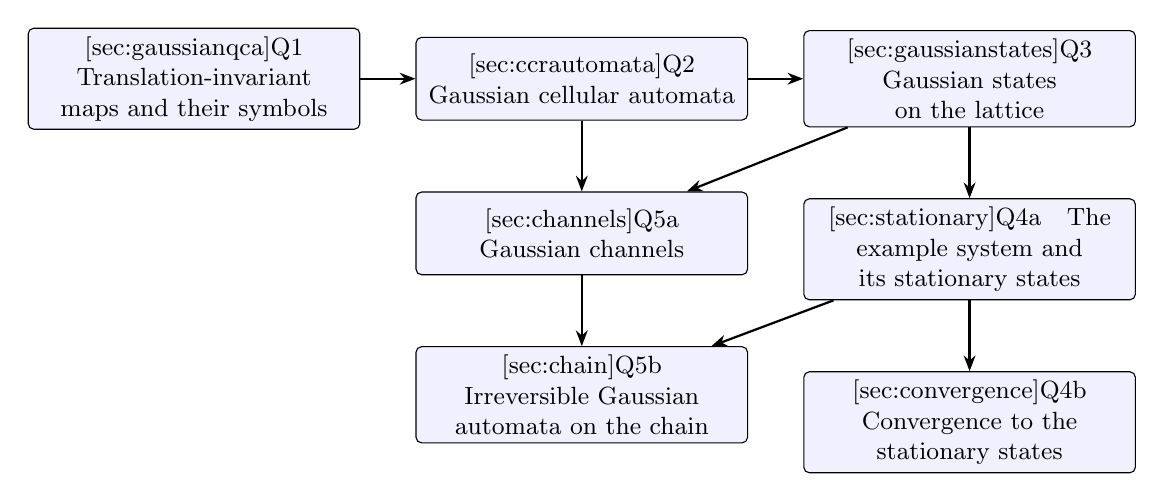
\begin{tikzpicture}[
  font=\small,
  done/.style={draw, rounded corners=2pt, fill=Blue!6, text width=4cm, align=center, execute at begin node={\hyphenpenalty=10000\relax},
    minimum height=1.05cm, inner sep=3pt},
  plan/.style={done, dashed, fill=none},
  dep/.style={-{Stealth[length=2mm]}, thick},
  node distance=0.9cm and 0.7cm]
  \node[done] (c1) {\hyperref[sec:gaussianqca]{Q1\quad Translation-invariant maps and their symbols}};
  \node[done, right=of c1] (c2) {\hyperref[sec:ccrautomata]{Q2\quad Gaussian cellular automata}};
  \node[done, right=of c2] (c3) {\hyperref[sec:gaussianstates]{Q3\quad Gaussian states on the lattice}};
  \node[done, below=of c3] (c4)
    {\hyperref[sec:stationary]{Q4a\quad The example system and its stationary states}};
  \node[done, below=of c4] (c4b) {\hyperref[sec:convergence]{Q4b\quad Convergence to the stationary states}};
  \node[done, below=of c2] (c5) {\hyperref[sec:channels]{Q5a\quad Gaussian channels}};
  \node[done, below=of c5] (c5b)
    {\hyperref[sec:chain]{Q5b\quad Irreversible Gaussian automata on the chain}};
  \draw[dep] (c1) -- (c2);
  \draw[dep] (c2) -- (c3);
  \draw[dep] (c3) -- (c4);
  \draw[dep] (c4) -- (c4b);
  \draw[dep] (c2) -- (c5);
  \draw[dep] (c3) -- (c5);
  \draw[dep] (c5) -- (c5b);
  \draw[dep] (c4) -- (c5b);
\end{tikzpicture}
\caption{Milestones and their dependence. Each box links to its chapter.}
\label{fig:roadmap}
\end{figure}

\clearpage
\section{Translation-invariant maps and their symbols}\label{sec:gaussianqca}

\noindent\motiv{\reve{A Gaussian cellular automaton acts on Weyl operators through a linear map $L$
of the classical phase space of a lattice. Three properties are required of $L$: it preserves the
symplectic form, so that it defines an automorphism of the CCR algebra; it commutes with the
lattice translations; and it moves each vector by a bounded distance.}}

\medskip
\noindent\motiv{\reve{This chapter shows that translation invariance turns $L$ into a matrix over
a ring of Laurent polynomials, its \emph{symbol}, and that preservation of the form becomes a
matrix identity for the symbol. For one mode per site and nearest-neighbour coupling the identity
is solved completely. The running example is one time step of the lattice Klein--Gordon
field.}}

\medskip
\noindent\motiv{\reve{The first three subsections work over a commutative ring $R$ and an abelian
group $G$, since the same algebra describes Clifford cellular automata over finite
fields~\cite{svw}. From Subsection~\ref{sec:nn} on, $R=\R$ and $G=\Z$.}}

\subsection{Lattice phase space}\label{sec:qca-space}

\noindent\motiv{\reve{The \emph{cell} is a finite set $\iota$ indexing the degrees of freedom at one
site; for $n$ bosonic modes, $\iota=\{q_1,\dots,q_n,p_1,\dots,p_n\}$. The group algebra $R[G]$ is the
ring of finite sums
\[c=\sum_{a\in G}c_a\,z^a,\qquad c_a\in R,\qquad z^az^b=z^{a+b}.\]
For $G=\Z$ these are the Laurent polynomials in $z$. The coefficient at the origin is
written $\varepsilon(c)=c_0$.}}

\begin{definition}[Lattice phase space]\label{def:qca-space}
The \emph{lattice phase space} is $V=R[G]^\iota$, the vectors $u=(u_i)_{i\in\iota}$ with
$u_i\in R[G]$. The \emph{value} of $u$ at $x\in G$ is $u(x)=\big((u_i)_x\big)_{i\in\iota}\in
R^\iota$, and the \emph{support} of $u$ is the finite set $\supp u=\{x\in G:u(x)\neq0\}$.
Translation by $a\in G$ is multiplication by $z^a$, written $\kappa_{a*}u=z^au$.
\end{definition}

\noindent\motiv{\reve{Reading $u$ through its values identifies $V$ with the finitely supported
functions $G\to R^\iota$. Multiplication by $z^a$ shifts the values forward:
\[(\kappa_{a*}u)(x)=u(x-a).\]
For example, with one mode and $G=\Z$, the vector with position $1$ at the site $0$ and momentum $2$
at the site $3$ is $u=(1,\,2z^3)$, and $\kappa_{1*}u=(z,\,2z^4)$ has the same values at the sites
$1$ and $4$.}}

\subsection{Translation-invariant maps and symbols}

\begin{definition}\label{def:qca-invariant}
An $R$-linear map $L\colon V\to V$ is \emph{translation invariant} if
$L\kappa_{a*}=\kappa_{a*}L$ for every $a\in G$.
\end{definition}

\begin{theorem}[Symbols]\label{thm:qca-symbol}
\begin{enumerate}[label=(\alph*)]
\item An $R$-linear map $L\colon V\to V$ is translation invariant if and only if it is
$R[G]$-linear.
\item The $R[G]$-linear maps $V\to V$ are the maps $u\mapsto\hat Lu$ with $\hat L\in
M_\iota(R[G])$, and $L\mapsto\hat L$ is an isomorphism of $R[G]$-algebras. In particular the
symbol of a composite $L_2L_1$ is the product $\hat L_2\hat L_1$.
\item Write $\hat L=\sum_m\ell_mz^m$ with coefficient matrices $\ell_m\in M_\iota(R)$, finitely
many nonzero. Then
\[(Lu)(x)=\sum_{m\in G}\ell_m\,u(x-m).\]
\end{enumerate}
The matrix $\hat L$ is the \emph{symbol} of $L$.
\end{theorem}

\begin{proof}\leavevmode
\begin{enumerate}[label=(\alph*)]
\item Multiplication by $z^a$ is $\kappa_{a*}$, so an $R[G]$-linear map is translation invariant.
Conversely, if $L$ is translation invariant and $c=\sum_ac_az^a$, then
$L(cu)=\sum_ac_aL(z^au)=\sum_ac_az^aLu=c\,Lu$.
\item $V$ is a free $R[G]$-module with basis $(e_i)_{i\in\iota}$. The endomorphisms of a free
module of finite rank over a commutative ring are the square matrices, and composition is the
matrix product.
\item $(Lu)_i=\sum_j\hat L_{ij}u_j$, and the coefficient at $x$ of a product in $R[G]$ is
$(\hat L_{ij}u_j)_x=\sum_m(\hat L_{ij})_m(u_j)_{x-m}$.
\end{enumerate}
\end{proof}

\noindent\motiv{\reve{By (c), the coefficient $\ell_m$ carries the value at $x-m$ to the value at
$x$. The simplest example is the shift $(Lu)(x)=u(x-1)$, with $\ell_1=1$ and symbol $z\cdot1$.}}

\begin{example}[The leapfrog rule]\label{ex:qca-leapfrog-rule}
The lattice Klein--Gordon equation for $\varphi\colon\Z^2\to\R$, with points $(t,x)$ and a
parameter $m^2\in\R$, is
\[\varphi(t+1,x)+\varphi(t-1,x)-\varphi(t,x+1)-\varphi(t,x-1)+m^2\varphi(t,x)=0 .\]
Given the values on two consecutive time slices,
\[d_0(x)=\varphi(t,x),\qquad d_1(x)=\varphi(t+1,x),\]
the equation at time $t+1$ determines the next slice:
\[d_2(x)=\varphi(t+2,x)=-d_0(x)+d_1(x+1)+d_1(x-1)-m^2d_1(x).\]
One time step is the map $F\colon(d_0,d_1)\mapsto(d_1,d_2)$. Take one mode per site with the cell
$u(x)=(d_0(x),d_1(x))$. Comparing
\[(Fu)(x)=\begin{pmatrix}d_1(x)\\-d_0(x)-m^2d_1(x)+d_1(x+1)+d_1(x-1)\end{pmatrix}\]
with Theorem~\ref{thm:qca-symbol}(c), the term $d_1(x+1)=u(x-(-1))_2$ comes from $\ell_{-1}$ and
$d_1(x-1)$ from $\ell_{+1}$, so
\[\ell_0=\begin{pmatrix}0&1\\-1&-m^2\end{pmatrix},\qquad
\ell_{-1}=\ell_{+1}=\begin{pmatrix}0&0\\0&1\end{pmatrix},\qquad
\hat F=\begin{pmatrix}0&1\\-1&z+z^{-1}-m^2\end{pmatrix}.\]
\end{example}

\noindent\motiv{\reve{Since only finitely many $\ell_m$ are nonzero, a translation-invariant map
moves every vector by a bounded distance.}}

\begin{corollary}[Finite range]\label{cor:qca-range}
Let $N=\bigcup_{i,j}\supp\hat L_{ij}$. Then $\supp Lu\subseteq\supp u+N$ for every $u\in V$.
\end{corollary}

\begin{proof}
If $(Lu)(x)\neq0$, then by Theorem~\ref{thm:qca-symbol}(c) some $\ell_mu(x-m)$ is nonzero, so
$m\in N$ and $x-m\in\supp u$.
\end{proof}

\noindent\motiv{\reve{For the leapfrog, $N=\{-1,0,1\}$: one step changes the Cauchy data only
within distance one of their support.}}

\subsection{Forms preserved by symbols}\label{sec:qca-forms}

\noindent\motiv{\reve{A form on one cell, given by a matrix $B\in M_\iota(R)$, defines a form on
$V$ by summing over sites. Writing it through symbols needs the \emph{involution} of $R[G]$, the
$R$-algebra automorphism
\[c\mapsto c^\star,\qquad (z^a)^\star=z^{-a}.\]
For a matrix $M$ over $R[G]$, $M^{\star\mathsf T}$ is the transpose of the matrix with entries
$M_{ij}^\star$. Since $R[G]$ is commutative, $(MN)^{\star\mathsf T}=N^{\star\mathsf T}M^{\star\mathsf
T}$.}}

\begin{definition}[Lifted form]\label{def:qca-lift}
For $B\in M_\iota(R)$, the \emph{lifted form} on $V$ is
\[\tilde B(u,w)=\sum_{x\in G}u(x)^{\mathsf T}B\,w(x)
=\varepsilon\Big(\sum_{i,j\in\iota}u_i^\star B_{ij}w_j\Big).\]
The matrix $B$ is \emph{alternating} if $v^{\mathsf T}Bv=0$ for every $v\in R^\iota$.
\end{definition}

\noindent\motiv{\reve{The two expressions agree because the coefficient of $u_i^\star w_j$ at the
origin is $\sum_x(u_i)_x(w_j)_x$. If $B$ is alternating, so is $\tilde B$. For $n$ bosonic modes
and $B=\Omega=\begin{psmallmatrix}0&I\\-I&0\end{psmallmatrix}$, the lifted form
$\sigma=\tilde\Omega$ is the symplectic form of the Notation table. (Alternating is stronger than
$B^{\mathsf T}=-B$ only when $2$ is not invertible, as for Clifford automata over $\Z/2$.)}}

\begin{theorem}[Twisted criterion]\label{thm:qca-criterion}
Let $B\in M_\iota(R)$ and let $L$ be translation invariant with symbol $\hat L$. Then
$\tilde B(Lu,Lw)=\tilde B(u,w)$ for all $u,w\in V$ if and only if
\[\hat L^{\star\mathsf T}B\,\hat L=B.\]
\end{theorem}

\begin{proof}
For $P\in M_\iota(R[G])$ put $\langle u,Pw\rangle=\varepsilon\big(\sum_{i,j}u_i^\star
P_{ij}w_j\big)$, so that $\tilde B(u,w)=\langle u,Bw\rangle$. The involution is a ring homomorphism
fixing $R$, so $(\hat Lu)_i^\star=\sum_k\hat L_{ik}^\star u_k^\star$, and therefore
$\tilde B(Lu,Lw)=\langle u,\hat L^{\star\mathsf T}B\hat Lw\rangle$. Invariance thus says
$\langle u,Qw\rangle=0$ for all $u,w$, where $Q=\hat L^{\star\mathsf T}B\hat L-B$. If $Q=0$ this
holds. Conversely, $u=e_i$ and $w=z^ke_j$ give
$\langle u,Qw\rangle=\varepsilon(Q_{ij}z^k)=(Q_{ij})_{-k}$, so every coefficient of every entry of
$Q$ vanishes.
\end{proof}

\noindent\motiv{\reve{Without the involution the criterion would fail for rules that move
vectors. For the shift $\hat L=z\cdot1$ one has $\hat L^{\star\mathsf T}B\hat L=z^{-1}Bz=B$, so the
shift preserves every lifted form; the plain transpose would give $z^2B$. Expanding
$\hat L^{\star\mathsf T}=\sum_m\ell_m^{\mathsf T}z^{-m}$ and collecting the coefficient of $z^k$
gives the criterion in coefficients:
\begin{equation}\label{eq:qca-coeff}
\sum_{m}\ell_m^{\mathsf T}B\,\ell_{m+k}=\delta_{k0}B\qquad\text{for every }k\in G.
\end{equation}}}

\begin{example}[On-site rules]\label{ex:qca-onsite}
Let $\hat L=S$ be constant, with $n$ modes per cell and $S$ a real $2n\times2n$ matrix. Then
$\hat L^{\star\mathsf T}=S^{\mathsf T}$, so $L$ preserves $\sigma$ if and only if
$S^{\mathsf T}\Omega S=\Omega$. This is equivalent to $S\Omega S^{\mathsf T}=\Omega$: if
$S^{\mathsf T}\Omega S=\Omega$, then $S$ is invertible with $S^{\mathsf T}=\Omega S^{-1}\Omega^{-1}$,
and
\[S\Omega S^{\mathsf T}=S\Omega^2S^{-1}\Omega^{-1}=-\Omega^{-1}=\Omega,\]
using $\Omega^2=-1$; the converse is the same computation for $S^{\mathsf T}$.
\end{example}

\noindent\motiv{\reve{Under the condition $S\Omega S^{\mathsf T}=\Omega$ the map
\revt{$\gamma_B\mapsto S\gamma_BS^{\mathsf T}$ preserves the uncertainty relation $\gamma_B-\ii\Omega\geq0$ of
real symmetric covariance matrices; the automaton of the on-site rule $S$ itself moves covariance
matrices by $S^{-1}$, which is symplectic as well (Corollary~\ref{cor:gs-onsite}).}}}

\begin{example}[Coefficient form of the criterion]\label{ex:qca-coeff}
For $n$ modes \revt{on the chain, $G=\Z$ and $R=\R$,} and $\hat L=\sum_mz^m\ell_m$, put $\ell_m^+=\Omega^{-1}\ell_m^{\mathsf T}\Omega$, the
symplectic adjoint. Multiplying~\eqref{eq:qca-coeff} with $B=\Omega$ on the left by $\Omega^{-1}$,
$\hat L$ is symplectic if and only if
\[\sum_m\ell_m^+\ell_{m+k}=\delta_{k0}1\qquad\text{for every }k\in\Z.\]
\end{example}

\begin{theorem}[Inverse]\label{thm:qca-inverse}
Let $B$ be invertible and $\hat L^{\star\mathsf T}B\hat L=B$. Then $L$ is bijective. Its inverse
is translation invariant with symbol $B^{-1}\hat L^{\star\mathsf T}B$, preserves $\tilde B$, and
has finite range.
\end{theorem}

\begin{proof}
$(B^{-1}\hat L^{\star\mathsf T}B)\hat L=B^{-1}B=1$, so $B^{-1}\hat L^{\star\mathsf T}B$ is a left
inverse. A square matrix over a commutative ring with a left inverse has invertible determinant,
since $\det(PM)=\det P\det M=1$, so the left inverse is two-sided. The inverse $\hat N$ satisfies
$\hat N^{\star\mathsf T}B\hat N=\hat N^{\star\mathsf T}(\hat L^{\star\mathsf T}B\hat L)\hat N
=(\hat L\hat N)^{\star\mathsf T}B(\hat L\hat N)=B$, and it has finite range by
Corollary~\ref{cor:qca-range}.
\end{proof}

\noindent\motiv{\reve{On an infinite-dimensional phase space, a map preserving a nondegenerate
form is injective but need not be onto. For translation-invariant maps the theorem gives an
inverse, and the inverse again has finite range.}}

\begin{corollary}[The group of rules]\label{cor:qca-group}
For invertible $B$, the symbols $\hat L$ with $\hat L^{\star\mathsf T}B\hat L=B$ form a group under
multiplication.
\end{corollary}

\begin{proof}
They are invertible by Theorem~\ref{thm:qca-inverse}, which also shows that the inverse satisfies
the identity. The identity matrix satisfies it, and if $\hat L$ and $\hat N$ do, then
$(\hat L\hat N)^{\star\mathsf T}B\hat L\hat N=\hat N^{\star\mathsf T}(\hat L^{\star\mathsf T}B\hat L)\hat N=B$.
\end{proof}

\noindent\motiv{\reve{A rule preserving $\sigma$ satisfies $\sigma(Lu,Lw)=\sigma(u,w)$ for all
$u,w$, which is exactly what is needed for $W(u)\mapsto W(Lu)$ to extend to an automorphism of
$\CCR(V,\sigma)$.}}

\subsection{Nearest-neighbour rules on one mode}\label{sec:nn}

\noindent\motiv{\reve{From now on $R=\R$, $G=\Z$, and there is one mode per site, $\iota=\{q,p\}$, with
\[\Omega=\begin{pmatrix}0&1\\-1&0\end{pmatrix}.\]
A symbol is \emph{symplectic} if $\hat L^{\star\mathsf T}\Omega\hat L=\Omega$, and
\emph{nearest-neighbour} if
\[\hat L=\ell_-z^{-1}+\ell_0+\ell_+z,\qquad \ell_-,\ell_0,\ell_+\in M_2(\R),\]
so that $(Lu)(x)=\ell_-u(x+1)+\ell_0u(x)+\ell_+u(x-1)$. The leapfrog is of this form. For
$2\times2$ matrices the symplectic condition is governed by the adjugate
\[\operatorname{adj}\begin{pmatrix}a&b\\c&d\end{pmatrix}=\begin{pmatrix}d&-b\\-c&a\end{pmatrix},
\qquad A\operatorname{adj}A=\operatorname{adj}(A)A=(\det A)\,1.\]}}

\begin{lemma}[$2\times2$ identities]\label{lem:qca-2x2}
For $A,A'\in M_2(\R)$:
\begin{enumerate}[label=(\alph*)]
\item $A^{\mathsf T}\Omega A'=\Omega\operatorname{adj}(A)A'$, and in particular
$A^{\mathsf T}\Omega A=(\det A)\,\Omega$;
\item $\operatorname{adj}$ is additive, $\operatorname{adj}(AA')=\operatorname{adj}(A')\operatorname{adj}(A)$ and
$\operatorname{adj}\operatorname{adj}A=A$;
\item $\det(A+A')=\det A+\det A'+\operatorname{tr}(\operatorname{adj}(A)A')$;
\item if $\operatorname{adj}A=A$, then $A$ is a multiple of $1$.
\end{enumerate}
\end{lemma}

\begin{proof}\leavevmode
\begin{enumerate}[label=(\alph*)]
\item For $A=\begin{psmallmatrix}a&b\\c&d\end{psmallmatrix}$, both $A^{\mathsf T}\Omega$ and
$\Omega\operatorname{adj}(A)$ equal $\begin{psmallmatrix}-c&a\\-d&b\end{psmallmatrix}$; multiply on the
right by $A'$. For $A'=A$, use $\operatorname{adj}(A)A=(\det A)1$.
\item The entries of $\operatorname{adj}A$ are linear in those of $A$; we check the other two identities
on entries.
\item We check this on entries.
\item $\operatorname{adj}A=A$ says $-A_{12}=A_{12}$, $-A_{21}=A_{21}$ and $A_{22}=A_{11}$.
\end{enumerate}
\end{proof}

\noindent\motiv{\reve{Part~(d) uses $2\neq0$; over $\Z/2$ every matrix with equal diagonal entries
equals its adjugate. We therefore prove the classification below over $\R$ (any field of
characteristic other than $2$ would do).}}

\begin{proposition}[Coefficient equations]\label{prop:qca-C}
A nearest-neighbour symbol is symplectic if and only if the coefficients of $z^{2},z^{-2},z,
z^{-1},z^0$ in $\hat L^{\star\mathsf T}\Omega\hat L-\Omega$ vanish:
\begin{align*}
&(C_2)\ \ \ell_-^{\mathsf T}\Omega\ell_+=0,\qquad (C_{-2})\ \ \ell_+^{\mathsf T}\Omega\ell_-=0,\qquad
(C_1)\ \ \ell_-^{\mathsf T}\Omega\ell_0+\ell_0^{\mathsf T}\Omega\ell_+=0,\\
&(C_{-1})\ \ \ell_0^{\mathsf T}\Omega\ell_-+\ell_+^{\mathsf T}\Omega\ell_0=0,\qquad
(C_0)\ \ \ell_-^{\mathsf T}\Omega\ell_-+\ell_0^{\mathsf T}\Omega\ell_0+\ell_+^{\mathsf T}\Omega\ell_+=\Omega.
\end{align*}
\end{proposition}

\begin{proof}
$\hat L^{\star\mathsf T}=\ell_-^{\mathsf T}z+\ell_0^{\mathsf T}+\ell_+^{\mathsf T}z^{-1}$; multiply out
and collect powers of $z$.
\end{proof}

\noindent\motiv{\reve{By Lemma~\ref{lem:qca-2x2}(a), $(C_{\pm2})$ say
$\operatorname{adj}(\ell_\mp)\ell_\pm=0$, and $(C_0)$ says $\det\ell_-+\det\ell_0+\det\ell_+=1$.
We can read off two families of solutions:
\begin{itemize}
\item the \emph{pure shifts} $Sz^{-1}$ and $Sz$ with $\det S=1$, where $\ell_0=0$;
\item $\ell_0\in SL_2(\R)$ and $\ell_+=\ell_-=\ell$ with $\det\ell=0$; then $(C_{\pm2})$ and $(C_0)$
hold, and $(C_{\pm1})$ is one remaining condition on $\ell$.
\end{itemize}
The next proposition shows that there are no others.}}

\begin{proposition}[Classification of nearest-neighbour rules]\label{prop:qca-nn}
A nearest-neighbour symbol is symplectic if and only if one of the following holds:
\begin{enumerate}[label=(\roman*)]
\item $\ell_0=0$, and either $\ell_+=0$ and $\det\ell_-=1$, or $\ell_-=0$ and $\det\ell_+=1$;
\item $\det\ell_0=1$, $\ell_+=\ell_-$, $\det\ell_+=0$, and
$\ell_+^{\mathsf T}\Omega\ell_0+\ell_0^{\mathsf T}\Omega\ell_+=0$.
\end{enumerate}
\end{proposition}

\begin{proof}
The two families above show that (i) and (ii) are symplectic; in (ii), $(C_{-1})$ is $(C_1)$ with
the two terms exchanged. Conversely, assume the equations $(C)$.

\emph{$\ell_-$ invertible.} $(C_2)$ gives $\ell_+=0$. Then $(C_1)$ reads
$\operatorname{adj}(\ell_-)\ell_0=0$, so $\ell_0=0$, and $(C_0)$ gives $\det\ell_-=1$: case (i).

\emph{$\ell_+$ invertible.} The same argument with $(C_{-2})$ and $(C_{-1})$ gives the other half
of case (i).

\emph{$\ell_-$ and $\ell_+$ both singular.} $(C_0)$ gives $\det\ell_0=1$, so
$\ell_0\operatorname{adj}\ell_0=1$. Put $D=\ell_--\ell_+$. Subtracting $(C_1)$ from $(C_{-1})$, in
the adjugate form of Lemma~\ref{lem:qca-2x2}(a), gives
$\operatorname{adj}(\ell_0)D=\operatorname{adj}(D)\ell_0$. For $K=\operatorname{adj}(\ell_0)D$,
Lemma~\ref{lem:qca-2x2}(b) and this identity give
\[\operatorname{adj}K=\operatorname{adj}(D)\,\ell_0=\operatorname{adj}(\ell_0)D=K,\]
so $K=c1$ for some $c\in\R$ by Lemma~\ref{lem:qca-2x2}(d), and $D=\ell_0K=c\,\ell_0$. Hence
$\det D=c^2$. On the other hand, Lemma~\ref{lem:qca-2x2}(c) with $A=\ell_-$, $A'=-\ell_+$ and
$(C_2)$ gives $\det D=\det\ell_-+\det\ell_+-\operatorname{tr}(\operatorname{adj}(\ell_-)\ell_+)=0$.
So $c=0$ and $\ell_+=\ell_-$: case (ii).
\end{proof}

\noindent\motiv{\reve{In case (ii) the last condition is one scalar equation. The identity
$\operatorname{adj}(A)A'+\operatorname{adj}(A')A=\operatorname{tr}(\operatorname{adj}(A)A')\,1$,
checked on entries, and Lemma~\ref{lem:qca-2x2}(a) give
$\ell^{\mathsf T}\Omega\ell_0+\ell_0^{\mathsf T}\Omega\ell=\operatorname{tr}(\operatorname{adj}(\ell_0)\ell)\,\Omega$,
so the condition is $\operatorname{tr}(\operatorname{adj}(\ell_0)\ell)=0$.}}

\begin{remark}[Pure shifts]\label{rem:qca-shift}
\reve{Case (i) contains the translation $z^{\pm1}\cdot1$, which moves the state of every cell one site
along the chain. It is a symplectic nearest-neighbour rule with one mode per site and $\ell_0=0$,
and it is not of the form (ii).}
\end{remark}

\noindent\motiv{\reve{In case (ii), $\det\ell=0$, so $\ell=va^{\mathsf T}$ for some vectors $v,a$, with
$v\neq0$ if $\ell\neq0$. A change of basis in the cell reduces to $v=e_1=(1,0)$, the position
direction: for $S\in SL_2(\R)$, the conjugation $\hat L\mapsto S\hat LS^{-1}$ maps symplectic symbols
to symplectic symbols (Corollary~\ref{cor:qca-group} with Example~\ref{ex:qca-onsite}), replaces
$v$ by $Sv$, and replaces $\ell_0$ by $S\ell_0S^{-1}$. For $v=e_1$ the last condition fixes $a$.}}

\begin{proposition}[Coupling in a fixed direction]\label{prop:qca-form}
Let $\det\ell_0=1$ and let $r$ be the second row of $\ell_0$. For $a\in\R^2$, the symbol with
$\ell_+=\ell_-=e_1a^{\mathsf T}$, which satisfies all conditions of case (ii) except the last, is
symplectic if and only if $a=\lambda r$ for some $\lambda\in\R$.
\end{proposition}

\begin{proof}
Write $\ell=e_1a^{\mathsf T}$. Since $e_1^{\mathsf T}\Omega=e_2^{\mathsf T}$ and $\Omega e_1=-e_2$,
\[\ell^{\mathsf T}\Omega\ell_0=a\,e_2^{\mathsf T}\ell_0=ar^{\mathsf T},\qquad
\ell_0^{\mathsf T}\Omega\ell=-\ell_0^{\mathsf T}e_2a^{\mathsf T}=-ra^{\mathsf T}.\]
So the last condition of case (ii) reads $ar^{\mathsf T}=ra^{\mathsf T}$, which holds if and only if
$a=\lambda r$, since $r\neq0$. The other conditions of case (ii) hold because
$\det(e_1a^{\mathsf T})=0$.
\end{proof}

\noindent\motiv{\reve{The number $\lambda$ is the \emph{coupling} of the rule.}}

\begin{example}[The leapfrog step is symplectic]\label{ex:qca-leapfrog}
For every real $m^2$, the leapfrog symbol $\hat F$ of Example~\ref{ex:qca-leapfrog-rule} and
\[\hat F^{-1}=\begin{pmatrix}z+z^{-1}-m^2&-1\\1&0\end{pmatrix}\]
are symplectic, and $\hat F\hat F^{-1}=1$.
\end{example}

\noindent\motiv{\reve{Both lie in case (ii) of Proposition~\ref{prop:qca-nn}: for $\hat F$,
$\det\ell_0=1$, $\det\ell_\pm=0$, and the last condition holds; the same computation applies to
$\hat F^{-1}$. In the Cauchy data $(d_0,d_1)$, the form
$\sigma(u,u')=\sum_x\big(d_0(x)d_1'(x)-d_1(x)d_0'(x)\big)$ is the conserved Wronskian of the lattice
Klein--Gordon equation, so $d_0$ plays the role of position and $d_1$ of momentum. The inverse
$\hat F^{-1}$ has $\ell_\pm=e_1e_1^{\mathsf T}$; it is Proposition~\ref{prop:qca-form} with $r=e_1$
and $\lambda=1$. For $\hat F$ itself, $\ell_\pm=e_2e_2^{\mathsf T}$ points in the momentum direction, so
Proposition~\ref{prop:qca-form} applies to it only after the change of basis described before
that proposition.}}

\subsection{Fourier modes}\label{sec:qca-fourier}

\noindent\motiv{\reve{Evaluating a symbol on the unit circle gives its Fourier transform: the
formula of Theorem~\ref{thm:qca-symbol}(c), applied to a plane wave $u(x)=e^{\ii kx}v$ with
$v\in\C^\iota$, gives $(Lu)(x)=e^{\ii kx}\hat L(e^{-\ii k})v$.}}

\begin{lemma}[Evaluation on the circle]\label{lem:qca-circle}
For $k\in\R$, evaluation at $z=e^{-\ii k}$ is a ring homomorphism from the Laurent polynomials
$\R[z,z^{-1}]$ to $\C$, with $p(e^{-\ii k})=\sum_mp_me^{-\ii km}$, and it carries the involution to
complex conjugation: $p^\star(e^{-\ii k})=\overline{p(e^{-\ii k})}$.
\end{lemma}

\begin{proof}
$e^{-\ii k}$ is a unit of $\C$, and a Laurent polynomial ring maps to any ring by sending $z$ to a
unit. On monomials, $(z^m)^\star=z^{-m}\mapsto e^{\ii km}=\overline{e^{-\ii km}}$, and the
coefficients are real.
\end{proof}

\noindent\motiv{\reve{The \emph{Fourier symbol} is $\hat L(k)=\hat L(e^{-\ii k})\in M_\iota(\C)$,
evaluated entrywise. By the lemma, $\hat L^{\star\mathsf T}$ evaluates to the conjugate transpose
$\hat L(k)^\dagger$.}}

\begin{example}[Fourier modes]\label{ex:qca-modes}
If $\hat L$ is symplectic, then
\[\hat L(k)^\dagger\,\Omega\,\hat L(k)=\Omega\qquad\text{for every }k\in\R.\]
For the leapfrog, $\operatorname{tr}\hat F(k)=2\cos k-m^2$.
\end{example}

\noindent\motiv{\reve{The conjugate transpose cannot be replaced by the transpose: for the shift
$\hat L=z\cdot1$, $\hat L(k)^{\mathsf T}\Omega\hat L(k)=e^{-2\ii k}\Omega$. The converse also holds:
if $\hat L(k)^\dagger\Omega\hat L(k)=\Omega$ for all $k$, each entry of
$\hat L^{\star\mathsf T}\Omega\hat L-\Omega$ is a Laurent polynomial vanishing at infinitely many points,
hence zero.}}

\begin{example}[Rotation with symmetric coupling]\label{ex:qca-rotation}
Let $\ell_0$ be the rotation by $\varphi$, with second row $r=(\sin\varphi,\cos\varphi)$, and
$\ell_\pm=\lambda\,e_1r^{\mathsf T}$ as in Proposition~\ref{prop:qca-form}:
\[\ell_0=\begin{pmatrix}\cos\varphi&-\sin\varphi\\ \sin\varphi&\cos\varphi\end{pmatrix},\qquad
\ell_\pm=\lambda\begin{pmatrix}\sin\varphi&\cos\varphi\\0&0\end{pmatrix}.\]
The rule is symplectic for all $\varphi$ and $\lambda$, and
\[\operatorname{tr}\hat L(k)=2\cos\varphi+2\lambda\cos k\sin\varphi.\]
\end{example}

\noindent\motiv{\reve{The trace comes from $\hat L(k)=\ell_0+2\cos k\,\ell_\pm$. Since $\det\hat L(k)=1$, writing $\operatorname{tr}\hat L(k)=2\cos\theta(k)$ \revt{where $|\operatorname{tr}\hat L(k)|\le2$}
gives the dispersion relation \reve{$\cos\theta(k)=\cos\varphi+\lambda\cos k\sin\varphi$}.}}

\subsection{Notes and references}\label{sec:qca-thesis}

\noindent\motiv{\reve{The material of this chapter is the phase-space part of Chapter~4
of~\cite{krueger}.}}

\begin{enumerate}
\item \reve{\emph{Conventions.} In~\cite{krueger} a rule is written
$(\Gamma\xi)_x=\sum_z\Gamma_z\xi_{x-z}$ (4.8), so $\Gamma_z=\ell_z$, and its Fourier transform
$\hat\Gamma(k)=\sum_x\Gamma_xe^{-\ii kx}$ (4.14)--(4.15) is $\hat L(e^{-\ii k})$. Translations there
act by $(\tau_\Delta\xi)_x=\xi_{x+\Delta}$ (p.~78), which is $\kappa_{a*}$ with $a=-\Delta$.}
\item \reve{\emph{Corresponding equations.} Theorem~\ref{thm:qca-symbol}(b),(c) are (4.13) and (4.8)
of~\cite{krueger}; Proposition~\ref{prop:qca-C} is (4.11); Example~\ref{ex:qca-coeff} is (4.10),
with $\Gamma^+$ the symplectic adjoint (2.1); Proposition~\ref{prop:qca-form} is (4.12), in the basis
of footnote~6 (p.~80), with the coupling written $f$; Example~\ref{ex:qca-rotation} is
(4.18)--(4.19); Example~\ref{ex:qca-modes} is the statement on p.~82 that $\hat\Gamma(k)$ ``induces a
symplectic transformation on every single mode $k$''.}
\item \reve{\emph{Range.} In~\cite[p.~92]{krueger} the condition $\Gamma_x=0$ for $x\notin N$ is
imposed on a rule. By Theorem~\ref{thm:qca-symbol}(c) it holds for every translation-invariant map,
with $N$ as in Corollary~\ref{cor:qca-range}.}
\item \reve{\emph{Invertibility.} \cite[p.~78]{krueger} states that $\Gamma$ is invertible ``as a
symplectic transformation''; Theorem~\ref{thm:qca-inverse} proves this for translation-invariant
rules.}
\item \reve{\emph{Pure shifts.} Proposition~4.4 of~\cite{krueger} derives from $(C_{\pm2})$ that
``$\Gamma_-$ and $\Gamma_+$ project onto the same, one-dimensional subspace'' (p.~80), which assumes
that both are nonzero, and so omits case (i) of Proposition~\ref{prop:qca-nn}. The Remark after it,
``the left- and right-shifter mentioned as examples in the introduction cannot be realized with one
mode per site'' (p.~80; the shifters are listed on p.~70), is contradicted by
Remark~\ref{rem:qca-shift}.}
\item \reve{\emph{Direction of time.} For the lattice Klein--Gordon field, the forward rule in the
convention of~\cite{krueger} corresponds to $F^{-1}$; this is made precise in \reve{Proposition~\ref{prop:time-direction}}.}
\end{enumerate}

\clearpage
\section{Gaussian cellular automata}\label{sec:ccrautomata}

\noindent\motiv{\reve{Chapter~\ref{sec:gaussianqca} studied rules acting on the phase space itself; this chapter
lets them act instead on the observables. A symplectic rule $L$ defines an automorphism $\alpha_L$ of
the CCR algebra by $\alpha_L(W(u))=W(Lu)$, and this automorphism is local, commutes with the lattice
translations, and composes, so that it is a quantum cellular automaton in the sense made precise
below. Conversely, any automorphism sending Weyl operators to multiples of Weyl operators arises from
a symplectic linear bijection of $V$ together with a character, and the bijection is a rule
whenever the automorphism also commutes with the translations. The leapfrog again serves as the
running example, and at the end of the chapter it is identified with one time step of the lattice
Klein--Gordon field.}}

\medskip
\noindent\motiv{\reve{Throughout this chapter $G$ is an abelian group, the cell carries $n$ modes, and $V$ denotes
the lattice phase space of Definition~\ref{def:qca-space} over $\R$, equipped with the symplectic
form $\sigma=\tilde\Omega$. The algebra $\CCR(V,\sigma)$ is the C*-algebra generated by the Weyl
operators $W(u)$ on $\ell^2(V)$, which act by
\[(W(u)f)(v)=e^{\ii\sigma(u,v)/2}f(v+u),\]
and consequently satisfy
\[W(u)W(w)=e^{-\ii\sigma(u,w)/2}\,W(u+w),\qquad W(u)^*=W(-u).\]} \reve{Here $\ell^2(V)$ is the space of
square-summable functions on the set $V$, with the point masses $\delta_v$ as orthonormal basis; it
serves only to construct the algebra, and it is not the Fock space of the oscillators, since
$t\mapsto W(tu)$ is not continuous on it and it carries no Gaussian state
(Remark~\ref{rem:gs-existence}). The algebra, and not this representation, is what the states and
channels of later chapters act on.}}

\subsection{The lattice CCR net}

\noindent\motiv{\reve{Local observables are attached to regions of the lattice, understood as subsets
$O\subseteq G$: observables belonging to disjoint regions should commute, and the observables of a
region belong as well to every larger region containing it. Since the lattice carries no time
direction, there is no time-slice condition beyond this isotony.}}

\noindent\motiv{\reve{Every linear bijection of $V$ that preserves $\sigma$ relabels the Weyl operators, and both
the translations and the rules of the previous chapter are bijections of this kind.}}

\begin{lemma}[Relabelling]\label{lem:relabel}
Let $P\colon V\to V$ be a linear bijection with \reve{$\sigma(Pu,Pw)=\sigma(u,w)$}. The unitary
$(U_P\psi)(v)=\psi(P^{-1}v)$ on $\ell^2(V)$ satisfies $U_PW(u)U_P^*=W(Pu)$, so $\alpha_P=U_P\,\cdot\,U_P^*$ is a
$*$-automorphism of $\CCR(V,\sigma)$ with $\alpha_P(W(u))=W(Pu)$, and $\alpha_{PP'}=\alpha_P\alpha_{P'}$.
\end{lemma}

\begin{proof}
$U_P$ is unitary because $P$ is a bijection, and $(U_P^*\psi)(v)=\psi(Pv)$. Hence
\[(U_PW(u)U_P^*\psi)(v)=e^{\ii\sigma(u,P^{-1}v)/2}\,\psi(v+Pu)=e^{\ii\sigma(Pu,v)/2}\,\psi(v+Pu)=(W(Pu)\psi)(v).\]
Conjugation by $U_P$ is a $*$-automorphism of the bounded operators, isometric, and maps the Weyl
operators onto the Weyl operators; so it maps $\CCR(V,\sigma)$, the closure of their span, onto
itself. Finally $U_{PP'}=U_PU_{P'}$. Two automorphisms that agree on the Weyl operators agree on
their span, and so on its closure; so $\alpha_P$ is the only automorphism with
$\alpha_P(W(u))=W(Pu)$.
\end{proof}

\begin{definition}[The lattice CCR net]\label{def:ccr-net}
For $O\subseteq G$, $\cA(O)$ is the closed $*$-subalgebra of $\CCR(V,\sigma)$ generated by the $W(u)$
with $\supp u\subseteq O$. The translation by $a\in G$ acts by $\alpha_a=\alpha_{\kappa_{a*}}$, so
$\alpha_a(W(u))=W(\kappa_{a*}u)$.
\end{definition}

\begin{theorem}\label{thm:ccr-net}
The net $O\mapsto\cA(O)$ is isotone, generates $\CCR(V,\sigma)$, and satisfies causality: elements of
$\cA(O_1)$ and $\cA(O_2)$ commute when $O_1\cap O_2=\emptyset$. The map $a\mapsto\alpha_a$ is a group
homomorphism into the automorphisms of $\CCR(V,\sigma)$, and $\alpha_a\cA(O)=\cA(O+a)$.
\end{theorem}

\begin{proof}
\reve{Isotony holds because $\cA(O)$ has fewer generators than $\cA(O')$ whenever $O\subseteq O'$,
while $\cA(G)=\CCR(V,\sigma)$ by definition. For causality, if $\supp u\cap\supp w=\emptyset$ then
every term of $\sigma(u,w)=\sum_xu(x)^{\mathsf T}\Omega w(x)$ vanishes, so that $W(u)$ and $W(w)$ commute;
since the commutant of the generators of $\cA(O_2)$ is a closed $*$-algebra, being closed under $*$ as
a set, and contains the generators of $\cA(O_1)$, it contains $\cA(O_1)$ itself, and by the same
argument the commutant of $\cA(O_1)$ contains $\cA(O_2)$. For the last statement, translations
preserve $\sigma$, so $\alpha_a$ exists by Lemma~\ref{lem:relabel}, and $\alpha_{a+b}=\alpha_a\alpha_b$
because $\kappa_{(a+b)*}=\kappa_{a*}\kappa_{b*}$; since $\supp\kappa_{a*}u=\supp u+a$, $\alpha_a$
carries the generators of $\cA(O)$ onto those of $\cA(O+a)$, and being an isometric $*$-automorphism
it therefore carries $\cA(O)$ onto $\cA(O+a)$.}
\end{proof}

\subsection{The automorphism of a rule}

\noindent\motiv{\reve{Since a symplectic rule $L$ is a bijection of $V$ preserving $\sigma$
(Theorem~\ref{thm:qca-inverse}), Lemma~\ref{lem:relabel} already furnishes its automorphism
$\alpha_L$.}}

\begin{proposition}\label{prop:alpha}
For symplectic rules $L$ and $K$:
\begin{enumerate}[label=(\alph*)]
\item $\alpha_L(W(u))=W(Lu)$;
\item $\alpha_{LK}=\alpha_L\alpha_K$ and $\alpha_1=\mathrm{id}$;
\item $\alpha_L\alpha_a=\alpha_a\alpha_L$ for every $a\in G$;
\item $\alpha_L^{-1}=\alpha_{L^{-1}}$, where $L^{-1}$ has symbol $\Omega^{-1}\hat L^{\star\mathsf T}\Omega$.
\end{enumerate}
\end{proposition}

\begin{proof}
\begin{enumerate}[label=(\alph*)]
\item \reve{Lemma~\ref{lem:relabel}.}
\item \reve{Lemma~\ref{lem:relabel}.}
\item $L$ commutes with $\kappa_{a*}$ (Theorem~\ref{thm:qca-symbol}(a)), so both sides send $W(u)$ to
$W(L\kappa_{a*}u)$.
\item By (b) and Theorem~\ref{thm:qca-inverse}.
\end{enumerate}
\end{proof}

\begin{theorem}[Locality]\label{thm:alpha-local}
Let $N$ be the range of the symbol of $L$. Then $\alpha_L\cA(O)\subseteq\cA(O+N)$ for every $O\subseteq G$.
\end{theorem}

\begin{proof}
If $\supp u\subseteq O$, then $\supp Lu\subseteq O+N$ (Corollary~\ref{cor:qca-range}), so $\alpha_L$ maps
the generators of $\cA(O)$ into $\cA(O+N)$. A $*$-homomorphism maps the $*$-algebra generated by a set
onto the $*$-algebra generated by its image; a $*$-automorphism of a C*-algebra is isometric, so it
maps closures into closures, and $\cA(O+N)$ is closed.
\end{proof}

\subsection{Quantum cellular automata}

\begin{definition}[Reversible quantum cellular automaton]\label{def:rqca}
Let $\cA$ be a net over the subsets of $G$ in a C*-algebra $A$, with a group homomorphism
$a\mapsto\alpha_a$ into the automorphisms of $A$ such that $\alpha_a\cA(O)=\cA(O+a)$. A \emph{reversible quantum cellular automaton} is a
$*$-automorphism $T$ of $A$ together with a finite set $N\subseteq G$, its \emph{neighbourhood}, such
that $T\alpha_a=\alpha_aT$ for all $a$ and $T\cA(O)\subseteq\cA(O+N)$ for all $O$.
\end{definition}

\noindent\motiv{\reve{The locality condition $T\cA(O)\subseteq\cA(O+N)$ requires that a
single step change the observables of a region only within the neighbourhood of that region.}}

\begin{proposition}[Composition]\label{prop:rqca-comp}
If $(T_1,N_1)$ and $(T_2,N_2)$ are reversible quantum cellular automata on the same net, so is
$(T_2T_1,N_1+N_2)$.
\end{proposition}

\begin{proof}
$T_2T_1$ commutes with every $\alpha_a$, and $T_2T_1\cA(O)\subseteq T_2\cA(O+N_1)\subseteq\cA(O+N_1+N_2)$.
\end{proof}

\begin{theorem}\label{thm:rule-qca}
For a symplectic rule $L$ with range $N$, $(\alpha_L,N)$ is a reversible quantum cellular automaton
on the lattice CCR net.
\end{theorem}

\begin{proof}
Proposition~\ref{prop:alpha}(c) and Theorem~\ref{thm:alpha-local}; $N$ is finite because the entries of
the symbol are finitely supported. \reve{The inverse $\alpha_{L^{-1}}$ is likewise a reversible quantum cellular automaton, with
neighbourhood $-N$, since the entries of $\Omega^{-1}\hat L^{\star\mathsf T}\Omega$ are, up to sign,
exactly those of $\hat L^{\star\mathsf T}$.}
\end{proof}

\begin{example}[The leapfrog]\label{ex:ccr-leapfrog}
The leapfrog $F$ of Example~\ref{ex:qca-leapfrog-rule} and its inverse give reversible quantum
cellular automata $\alpha_F$ and $\alpha_{F^{-1}}$ with neighbourhood $\{-1,0,1\}$, and
$\alpha_F^{-1}=\alpha_{F^{-1}}$. In the Cauchy data $u(x)=(d_0(x),d_1(x))$,
$\alpha_F(W(u))=W(Fu)$ with $(Fu)(x)=\big(d_1(x),\,-d_0(x)+d_1(x+1)+d_1(x-1)-m^2d_1(x)\big)$.
\end{example}

\begin{example}[Shifts]\label{ex:ccr-shift}
For $a\in G$, the symbol $z^a\cdot1$ gives the reversible quantum cellular automaton with
neighbourhood $\{a\}$ whose automorphism is the translation $\alpha_a$ itself.
\end{example}

\begin{example}[On-site rules]\label{ex:ccr-onsite}
For $G=\Z$ and a real $2n\times2n$ matrix $S$ with $S\Omega S^{\mathsf T}=\Omega$, the constant symbol $S$ gives a
reversible quantum cellular automaton with neighbourhood $\{0\}$: every site evolves separately by
$S$. For one mode this covers the rotations $R_\varphi=\begin{psmallmatrix}\cos\varphi&-\sin\varphi\\
\sin\varphi&\cos\varphi\end{psmallmatrix}$, the free evolution of uncoupled oscillators, and the
squeezings $\operatorname{diag}(e^r,e^{-r})$, which iterated squeeze every site further.
\end{example}

\begin{example}[Rotation with symmetric coupling]\label{ex:ccr-rotation}
The rule of Example~\ref{ex:qca-rotation} gives a reversible quantum cellular automaton with
neighbourhood $\{-1,0,1\}$ for all $\varphi$ and $\lambda$. \reve{A neighbourhood need not be the smallest possible one, as is seen already at $\lambda=0$,
where the range of the symbol reduces to $\{0\}$.}
\end{example}

\subsection{The local rule}

\noindent\motiv{\reve{A rule is entirely determined by its action on the degrees of freedom of a single site. For
$i\in\iota$, let $u_i\in V$ denote the vector taking the value $e_i$ at the site $0$ and vanishing
elsewhere, so that the operators $W(tu_i)$, $t\in\R$, are precisely the Weyl operators of the site
$0$.}}

\begin{proposition}\label{prop:local-rule}
\begin{enumerate}[label=(\alph*)]
\item A \reve{translation-invariant linear map} is determined by the vectors $Lu_i$, $i\in\iota$.
\item A \reve{translation-invariant linear map} $L$ is symplectic if and only if
\[\sigma(Lu_i,\kappa_{x*}Lu_j)=\delta_{x0}\,\Omega_{ij}\qquad\text{for all }i,j\in\iota,\ x\in G.\]
\end{enumerate}
\end{proposition}

\begin{proof}
\begin{enumerate}[label=(\alph*)]
\item $Lu_i$ is the $i$-th column of the symbol \reve{(the vector whose value at $x\in G$ is $\hat L_{ji}$, read as a function on $G$), and the
symbol in turn determines $L$ by Theorem~\ref{thm:qca-symbol}.}
\item $\sigma(Lu_i,\kappa_{x*}Lu_j)$ is the coefficient of $(\hat L^{\star\mathsf T}\Omega\hat L)_{ij}$ at
$-x$, as in the proof of Theorem~\ref{thm:qca-criterion}; the condition says that this symbol is the
constant $\Omega$.
\end{enumerate}
\end{proof}

\noindent\motiv{\reve{In terms of the automaton, part (b) says that the images $\alpha_L(W(tu_i))=W(tLu_i)$ of the
one-site Weyl operators, together with their translates, satisfy the same commutation relations as
the one-site Weyl operators themselves.}}

\subsection{Automorphisms of Weyl type}

\noindent\motiv{\reve{The automorphisms of $\CCR(V,\sigma)$ that send every Weyl operator to a multiple of a Weyl
operator are characterized by means of a norm estimate. Let
$\delta_0\in\ell^2(V)$ be the unit vector at $0\in V$; the functional $\varphi(a)=(a\delta_0)(0)$
satisfies $|\varphi(a)|\le\|a\|$, and $\varphi(W(u))=1$ if $u=0$ and $0$ otherwise, since
$(W(u)\delta_0)(0)=\delta_0(u)$.}}

\begin{lemma}[Separation]\label{lem:separation}
If $y$ lies in the closed linear span of $\{W(v):v\neq u\}$, then $\|W(u)-y\|\ge1$. In particular,
$\mu W(u)=\nu W(w)$ with $\nu\neq0$ implies $u=w$ and $\mu=\nu$.
\end{lemma}

\begin{proof}
For $v\neq u$, $W(u)^*W(v)$ is a multiple of $W(v-u)$, so $\varphi(W(u)^*y')=0$ for $y'$ in the span and,
by continuity, in its closure, while $\varphi(W(u)^*W(u))=1$. Hence
$1=|\varphi(W(u)^*(W(u)-y))|\le\|W(u)-y\|$. For the second statement apply $\varphi(W(w)^*\,\cdot\,)$ to
both sides.
\end{proof}

\begin{theorem}\label{thm:weyl-type}
Let $T$ be a $*$-automorphism of $\CCR(V,\sigma)$, $Q\colon V\to V$ a map and $c\colon V\to\C$ with
$T(W(u))=c(u)W(Q u)$ for all $u$. Then $Q$ is a linear bijection with
$\sigma(Q u,Q w)=\sigma(u,w)$, and $c$ is a character: $c(u+w)=c(u)c(w)$, $|c(u)|=1$.
\end{theorem}

\begin{proof}
$c(u)\neq0$ since $T$ is injective, and $|c(u)|=1$ since $T$ is isometric and Weyl operators have
norm $1$.

\emph{Additivity.} Applying $T$ to $W(u)W(w)=e^{-\ii\sigma(u,w)/2}W(u+w)$ gives
\[c(u)c(w)\,e^{-\ii\sigma(Q u,Q w)/2}\,W(Q u+Q w)=e^{-\ii\sigma(u,w)/2}\,c(u+w)\,W(Q(u+w)),\]
so $Q(u+w)=Q u+Q w$ and the coefficients agree, by Lemma~\ref{lem:separation}.

\emph{Symplecticity.} Exchanging $u$ and $w$ and dividing gives $e^{-\ii\sigma(Q u,Q w)}=
e^{-\ii\sigma(u,w)}$, so $\sigma(u,w)-\sigma(Q u,Q w)=2\pi k(u,w)$ with $k(u,w)\in\Z$. By additivity,
$m\,Q(u/m)=Q u$ for $m\in\mathbb N$, hence $k(u,w)=m\,k(u/m,w)$; so $k(u,w)$ is divisible by every
$m$, and $k=0$.

\emph{Surjectivity.} If $v'\notin Q V$, then $T$ maps the span of the Weyl operators into the span
of $\{W(v):v\neq v'\}$. The Weyl operators span a dense subspace of $\CCR(V,\sigma)$ (their span is
already a $*$-algebra), and $T$ is continuous, so $W(v')=T(T^{-1}W(v'))$ lies in the closure of that
span, contradicting Lemma~\ref{lem:separation}.

\emph{Linearity.} For $t\in\R$, $\sigma(Q(tu)-tQ u,Q w)=\sigma(tu,w)-t\sigma(u,w)=0$ for every $w$;
since $Q$ is onto and $\sigma$ is nondegenerate (if $\sigma(u,w)=0$ for all $w$, pairing with the
one-site vectors $z^xe_j$ gives $\Omega^{\mathsf T} u(x)=0$ for every $x$, so $u=0$), $Q(tu)=tQ u$. If $Q u=0$ then
$\sigma(u,w)=0$ for all $w$, so $u=0$.

\emph{Character.} With symplecticity, the coefficient identity of the first step reads
$c(u)c(w)=c(u+w)$.
\end{proof}

\noindent\motiv{\reve{Nontrivial phases $c$ do occur in Theorem~\ref{thm:weyl-type}. For any character $c$ with $|c|=1$, the unitary
$(U\psi)(v)=\overline{c(v)}\,\psi(v)$ satisfies $UW(u)U^*=c(u)W(u)$, so that $\alpha_L$ followed by
conjugation with $U$ is an automorphism of the form of the theorem, with $Q=L$ and phase $c\circ L$.
When $T$ also commutes with the translations, comparing $T\alpha_a(W(u))$ with $\alpha_aT(W(u))$ shows
that $Q$ commutes with $\kappa_{a*}$, so that $Q$ is itself a rule and $c\circ\kappa_{a*}=c$. Such
translation-invariant characters do exist, for instance
$c(u)=\exp\big(\ii\sum_x\theta^{\mathsf T}u(x)\big)$ with $\theta\in\R^{2n}$, and conjugation with the
corresponding $U$ is a reversible quantum cellular automaton with neighbourhood $\{0\}$. The
translation-covariant automata of Weyl type are therefore exactly the automorphisms $\alpha_L$
followed by such a conjugation.}}

\subsection{The leapfrog and the direction of time}

\noindent\motiv{\reve{The Cauchy data $(d_0,d_1)$ of the lattice Klein--Gordon field form exactly the one-mode
lattice phase space over $\Z$, through $u(x)=(d_0(x),d_1(x))$, and their conserved form
$\sum_x\big(d_0(x)d_1'(x)-d_1(x)d_0'(x)\big)$ is $\sigma$. The leapfrog step $F$ of
Example~\ref{ex:qca-leapfrog-rule} advances the data from the slices $t,t+1$ to $t+1,t+2$, and it
remains to determine which automaton represents time evolution itself.}}

\begin{proposition}\label{prop:time-direction}
Let $\Lambda_t$ send a solution $\varphi$ of the lattice Klein--Gordon equation \reve{with finitely
supported Cauchy data} to its Cauchy data
$(\varphi(t,\cdot),\varphi(t+1,\cdot))$, and let $\tau$ translate solutions forward in time by one step,
$(\tau\varphi)(t,x)=\varphi(t-1,x)$. Then $\Lambda_t\tau=F^{-1}\Lambda_t$.
\end{proposition}

\begin{proof}
$\Lambda_t\tau\varphi=(\varphi(t-1,\cdot),\varphi(t,\cdot))=\Lambda_{t-1}\varphi$, and $\Lambda_t=F\Lambda_{t-1}$ by the
construction of $F$ in Example~\ref{ex:qca-leapfrog-rule}. Hence $\Lambda_{t-1}=F^{-1}\Lambda_t$.
\end{proof}

\noindent\motiv{\reve{Translating a solution forward in time shifts its Cauchy data at a fixed time backwards, and
on observables the consequence of this shift depends on how $W(u)$ is to be read. If $W(u)$ is
thought of as $e^{\ii\sigma(u,\Phi_t)}$, with $\Phi_t$ the Cauchy data of the quantum field at time
$t$ (a heuristic reading here, since $\ell^2(V)$ carries no field operators and $t\mapsto W(tu)$ is
not continuous), then the field moves as $\Phi_{t+1}=F\Phi_t$, so that
$\sigma(u,\Phi_{t+1})=\sigma(F^{-1}u,\Phi_t)$; under this reading the forward time step is therefore
the automaton $\alpha_{F^{-1}}$ of Example~\ref{ex:ccr-leapfrog}, rather than $\alpha_F$.}}

\subsection{Notes and references}\label{sec:ccr-notes}

\begin{enumerate}
\item \reve{\emph{Definition.} Definition~\ref{def:rqca} corresponds to Definition~4.1 of~\cite[p.~73]{krueger}
for reversible automata, with the quasi-local algebra there replaced by a net; the condition
$0\in N$ imposed in the thesis is not needed here. Irreversible automata, that is, quantum channels,
are treated \reve{in Chapter~\ref{sec:channels}}.}
\item \reve{\emph{Composition and local rule.} Proposition~\ref{prop:rqca-comp} corresponds to
Corollary~4.3 of the thesis. Proposition~\ref{prop:local-rule}(b) is the Gaussian analogue of
Lemma~4.2(ii) rather than a special case of it: that lemma, like the results
of~\cite{schumacher-werner}, concerns quasi-local algebras built from finite-dimensional cells,
whereas each cell here carries the Weyl algebra of $\R^{2n}$.}
\item \reve{\emph{Weyl-type automorphisms.} After (4.7), \cite[p.~78]{krueger} states that any $\Gamma$
for which $T(W(\xi))=W(\Gamma\xi)$ defines a homomorphism ``would have to be linear \dots\ and
fulfill $\sigma(\Gamma\xi,\Gamma\eta)=\sigma(\xi,\eta)$''. Theorem~\ref{thm:weyl-type} proves this claim
and additionally records the character $c$, which the thesis omits. Lemma~\ref{lem:relabel}, together
with the uniqueness of the CCR algebra for nondegenerate $\sigma$ (established in the proof of
Theorem~\ref{thm:weyl-type}), of which $\CCR(V,\sigma)$ is a concrete realization, is due to
Manuceau~\cite{manuceau}, Slawny~\cite{slawny}, and Manuceau, Sirugue, Testard and
Verbeure~\cite{mstv}; see~\cite[\S5.2]{bratteli-robinson}.}
\item \reve{\emph{Examples.} The thesis lists the free evolution, the left- and right-shifter, continued
squeezing, and symplectic rotations as examples of Gaussian automata (p.~70);
Example~\ref{ex:ccr-rotation} corresponds to its system (4.18).}
\item \reve{\emph{Direction of time.} In the convention $T(W(\xi))=W(\Gamma\xi)$ used in the thesis, the
rule governing the forward time step of the lattice Klein--Gordon field is $F^{-1}$.}
\end{enumerate}

\clearpage
\section{Gaussian states on the lattice}\label{sec:gaussianstates}

\noindent\motiv{\reve{The automata of Chapter~\ref{sec:ccrautomata} act on observables, and a
dynamics of observables becomes a dynamics of physical situations only once it acts on states. This
chapter introduces the states of the lattice CCR algebra through their characteristic functions,
singles out the Gaussian states, whose characteristic functions are exponentials of quadratic
forms, and derives the condition that the quadratic form of a Gaussian state must satisfy. Because
a Gaussian state is determined by a covariance form on the whole infinite lattice, whereas the
classical theory of Gaussian states concerns covariance matrices of finitely many modes, we devote a large
part of the chapter to showing that the two descriptions agree: restricted to a finite
region, a covariance form is a covariance matrix of finitely many modes, and the condition on the
form becomes the familiar matrix inequality on every region. On the chain the condition can also be
read off pointwise from a Fourier transform, which leads to a matrix condition that saturates the state condition at every wave number, and to an
explicit law for the evolution of the covariance under a Gaussian automaton.}}

\medskip
\noindent\motiv{\reve{As in Chapter~\ref{sec:ccrautomata}, $G$ is an abelian group, the cell carries
$n$ modes with coordinates ordered positions first, $u(x)=(q_1,\dots,q_n,p_1,\dots,p_n)$, and
$\sigma(u,w)=\sum_xu(x)^{\mathsf T}\Omega\,w(x)$ with
$\Omega=\begin{psmallmatrix}0&I_n\\-I_n&0\end{psmallmatrix}$, so that
$\Omega^{\mathsf T}=-\Omega=\Omega^{-1}$. For a site $x$ and a cell index $i$ we write $e_{x,i}\in V$
for the vector whose value at $x$ is the $i$-th unit vector and which vanishes elsewhere, so that
$\sigma(e_{x,i},e_{y,j})=\delta_{xy}\Omega_{ij}$. Since products and adjoints of Weyl operators are
multiples of Weyl operators, the linear span of the Weyl operators is a $*$-subalgebra of
$\CCR(V,\sigma)$, and it is dense by the definition of $\CCR(V,\sigma)$ as its closure. For a
complex vector or matrix, ${}^\dagger$ denotes the conjugate transpose, and $A\ge0$ means that the
Hermitian matrix $A$ is positive semidefinite.}}

\subsection{States and characteristic functions}

\noindent\motiv{\reve{A state assigns to each observable its expectation value, and the only
requirements on such an assignment are linearity, normalization and positivity on the squares
$a^*a$, which are the observables with non-negative spectrum.}}

\begin{definition}[State]\label{def:gs-state}
\reve{A \emph{state} on $\CCR(V,\sigma)$ is a continuous $\C$-linear functional $\omega$ with
$\omega(1)=1$ and $\omega(a^*a)\ge0$ for every $a$, where, for a complex number $z$, $z\ge0$ means that
$z$ is real and non-negative.}
\end{definition}

\noindent\reve{We require positivity of the complex numbers $\omega(a^*a)$, so that no order on
the algebra itself needs to be introduced. Continuity follows from positivity on every C*-algebra,
but it is included in the definition because it is the property the arguments below use directly.}

\noindent\motiv{\reve{Since the Weyl operators span a dense subalgebra, a continuous functional is
known once its values on them are known, and these values form a function on the phase space. The
products $W(u_j)^*W(u_k)$ are again multiples of Weyl operators, and positivity of the state on
combinations of such products becomes a positivity property of this function.}}

\begin{definition}[Characteristic function]\label{def:gs-chi}
\reve{The \emph{characteristic function} of a state $\omega$ is $\chi_\omega(u)=\omega(W(u))$. For a
function $\chi\colon V\to\C$ and a family $(u_j)_{j\in I}$ in $V$ indexed by a finite set $I$, the
\emph{twisted kernel} is the matrix
\[K_{jk}=e^{\ii\sigma(u_j,u_k)/2}\,\chi(u_k-u_j)\qquad(j,k\in I).\]}
\end{definition}

\begin{proposition}[Twisted positivity]\label{prop:gs-twisted}
\reve{Let $\omega$ be a state with characteristic function $\chi$.
\begin{enumerate}[label=(\alph*)]
\item For every finite family $(u_j)_{j\in I}$ and all $c\in\C^I$,
$\sum_{j,k}\bar c_jc_k\,e^{\ii\sigma(u_j,u_k)/2}\chi(u_k-u_j)\ge0$, so that the twisted kernel of
$\chi$ on every finite family is positive semidefinite.
\item $\chi(0)=1$, $\chi(-u)=\overline{\chi(u)}$ and $|\chi(u)|\le1$ for every $u\in V$.
\end{enumerate}}
\end{proposition}

\begin{proof}\leavevmode
\reve{\begin{enumerate}[label=(\alph*)]
\item By the Weyl relations,
$W(u_j)^*W(u_k)=W(-u_j)W(u_k)=e^{\ii\sigma(u_j,u_k)/2}W(u_k-u_j)$, so that for
$X=\sum_kc_kW(u_k)$ the product $X^*X$ equals
$\sum_{j,k}\bar c_jc_k\,e^{\ii\sigma(u_j,u_k)/2}W(u_k-u_j)$, and the sum in question is
$\omega(X^*X)\ge0$. A complex matrix $K$ whose quadratic form $c^\dagger Kc$ is real for every $c$
is Hermitian, because the quadratic form of $K-K^\dagger$, which is
$c^\dagger Kc-\overline{c^\dagger Kc}$, then vanishes identically, and a complex matrix with
vanishing quadratic form is zero by polarization. The twisted kernel is therefore Hermitian with
non-negative quadratic form, that is, positive semidefinite.
\item First, $\chi(0)=\omega(1)=1$. For the family $(0,u)$ the phases are trivial, because
$\sigma(0,u)=\sigma(u,0)=0$, and the twisted kernel is
$\begin{psmallmatrix}1&\chi(u)\\\chi(-u)&1\end{psmallmatrix}$. By (a) it is Hermitian, which gives
$\chi(-u)=\overline{\chi(u)}$, and its determinant $1-|\chi(u)|^2$ is non-negative.
\end{enumerate}}
\end{proof}

\begin{remark}[Twisted positive-definiteness]\label{rem:gs-bochner}
\reve{Part~(a) says that $\chi$ is \emph{$\sigma$-positive-definite}. For $\sigma=0$ this is the
positive-definiteness of Bochner's theorem, by which a continuous positive-definite function on a
finite-dimensional real vector space with $\chi(0)=1$ is the characteristic function of a
probability measure, and the twisted condition is its analogue for the canonical commutation
relations. The analogue of Bochner's theorem itself, for finitely many degrees of freedom, is the
quantum Bochner theorem of Kastler~\cite{kastler} and of Loupias and Miracle-Sole~\cite{lms}: a
continuous $\sigma$-positive-definite function on a finite-dimensional symplectic space with
$\chi(0)=1$ is the characteristic function of a density operator in the Schr\"odinger
representation, and its symplectic Fourier transform is the Wigner function of that density
operator, just as the Fourier transform of $\chi$ is the probability density in the commutative
case} \vetsource{(statement recalled, not checked against the two sources)}\reve{. Both hypotheses
of that theorem belong to finitely many degrees of freedom, continuity of $\chi$ and a Schr\"odinger
representation in which the density operator lives. On the infinite lattice there is no such
distinguished representation, and a state need not be given by a density operator in any fixed
representation, as Remark~\ref{rem:gs-existence} shows for the representation on $\ell^2(V)$. The
result that replaces the quantum Bochner theorem there is the characterization of states by their
characteristic functions quoted in that remark, which requires no continuity of $\chi$.}
\revs{This Fourier transform acts on the phase-space variable $u$, unlike the lattice Fourier
transform $x\mapsto k$ of Subsection~\ref{sec:gs-fourier}, which acts on the site variable of a
vector.}
\end{remark}

\noindent\motiv{\reve{Two properties of characteristic functions suffice for the evolution of
states: a state is determined by its characteristic function, and pulling a state back along an
automorphism that relabels the Weyl operators composes the characteristic function with the
relabelling.}}

\begin{proposition}[Pullback along automorphisms]\label{prop:gs-pullback}
\reve{\begin{enumerate}[label=(\alph*)]
\item Two states with the same characteristic function are equal.
\item If $\alpha$ is a $*$-automorphism of $\CCR(V,\sigma)$ and $\omega$ a state, then
$\omega\circ\alpha$ is a state. If in addition $\alpha(W(u))=W(Qu)$ for a map $Q\colon V\to V$, then
$\chi_{\omega\circ\alpha}=\chi_\omega\circ Q$.
\end{enumerate}}
\end{proposition}

\begin{proof}\leavevmode
\reve{\begin{enumerate}[label=(\alph*)]
\item Two continuous linear functionals that agree on the Weyl operators agree on their linear
span, and hence on its closure, which is the whole algebra.
\item A $*$-automorphism of a C*-algebra is isometric, so that $\omega\circ\alpha$ is continuous
as well as linear; it is normalized because $\alpha(1)=1$, and positive because
$\omega(\alpha(a^*a))=\omega(\alpha(a)^*\alpha(a))\ge0$. Finally
$\chi_{\omega\circ\alpha}(u)=\omega(W(Qu))=\chi_\omega(Qu)$.
\end{enumerate}}
\end{proof}

\begin{corollary}[Translation invariance]\label{cor:gs-transl}
\reve{A state $\omega$ satisfies $\omega\circ\alpha_a=\omega$ for every $a\in G$ if and only if
$\chi_\omega\circ\kappa_{a*}=\chi_\omega$ for every $a\in G$.}
\end{corollary}

\begin{proof}
\reve{By Proposition~\ref{prop:gs-pullback}(b) with $Q=\kappa_{a*}$, the state $\omega\circ\alpha_a$
has the characteristic function $\chi_\omega\circ\kappa_{a*}$, and by
Proposition~\ref{prop:gs-pullback}(a) it equals $\omega$ exactly when the two characteristic
functions agree.}
\end{proof}

\subsection{Gaussian states}

\noindent\motiv{\reve{In classical probability a Gaussian measure is one whose characteristic
function is the exponential of a quadratic polynomial, and the quantum definition takes over this
description word for word; on the CCR algebra these are the quasi-free states of Manuceau and
Verbeure~\cite{manuceau-verbeure}. The factor $\tfrac14$ in the exponent is the normalization in which the
vacuum of a single oscillator has covariance $1$, as Example~\ref{ex:gs-vacuum} below shows; it
agrees with the finite-mode convention in which the covariance matrix is twice the matrix of
symmetrized second moments.}}

\begin{definition}[Gaussian state]\label{def:gs-gaussian}
\reve{A \emph{Gaussian state} is a state $\omega$ together with a symmetric bilinear form $\gamma$ on
$V$, its \emph{covariance form}, and a linear form $d$ on $V$, its \emph{displacement}, such that
\[\chi_\omega(u)=\exp\bigl(\ii\,d(u)-\tfrac14\gamma(u,u)\bigr)\qquad\text{for all }u\in V.\]}
\end{definition}

\noindent\reve{Every result below concerns a Gaussian state given together with its data
$(\gamma,d)$. That a state with prescribed data exists is not proved in these notes, and no result
below depends on it; the examples of the chapter are accordingly covariance forms satisfying the
state condition of Definition~\ref{def:gs-statecond}, which by Theorem~\ref{thm:gs-necessity} is
necessary for a Gaussian state, and Remark~\ref{rem:gs-existence} explains why existence cannot
simply be read off from the construction of the algebra.}

\begin{remark}[The data are determined by the state]\label{rem:gs-data}
\reve{Although the definition lists $\gamma$ and $d$ as data, a state admits at most one pair of
them. Indeed, $|\chi_\omega(u)|=\exp(-\tfrac14\gamma(u,u))$ determines $\gamma(u,u)$ for every $u$,
and hence the symmetric form $\gamma$ by polarization; then
$\chi_\omega(tu)/|\chi_\omega(tu)|=e^{\ii t\,d(u)}$ for all $t\in\R$, and two real numbers $r,r'$
with $e^{\ii tr}=e^{\ii tr'}$ for every real $t$ are equal, as one sees by taking
$|t(r-r')|<2\pi$ with $t\neq0$, so that $d(u)$ is determined as well.}
\end{remark}

\begin{remark}[Normalizations]\label{rem:gs-normalization}
\reve{In the normalization of these notes $\chi_\omega(u)=\exp(\ii d(u)-\tfrac14\gamma(u,u))$, and
for one mode the corresponding covariance matrix $\gamma_B$ is twice the matrix of symmetrized
second moments, as the paragraph before Example~\ref{ex:gs-squeezed} shows. Other normalizations of the literature write the exponent with a
different constant, for instance as $-\tfrac12\gamma'(u,u)$, and then $\gamma=2\gamma'$; such a
rescaling of $\gamma$ by a constant makes conditions such as $\sigma(u,w)^2\le\gamma(u,u)\gamma(w,w)$
acquire factors, here $\tfrac14\sigma(u,w)^2\le\gamma'(u,u)\gamma'(w,w)$, without changing their
content. The sign of $\ii\Omega$ is likewise a matter of convention: for a real symmetric matrix
$\gamma_B$ of $M$ modes the matrices $\gamma_B-\ii\Omega_M$ and $\gamma_B+\ii\Omega_M$, with
$\Omega_M$ the symplectic matrix of \revt{Subsection}~\ref{sec:gs-regions}, are complex conjugates of each
other, and the complex conjugate of a positive semidefinite matrix is positive semidefinite, so
that $\gamma_B-\ii\Omega_M\ge0$ and $\gamma_B+\ii\Omega_M\ge0$ are equivalent and either may be called
the finite-mode condition.}
\end{remark}

\begin{remark}[Existence and regularity]\label{rem:gs-existence}
\reve{The representation of $\CCR(V,\sigma)$ on $\ell^2(V)$ by which the algebra was constructed
contains no Gaussian state. For $u\neq0$ and $t\neq0$, the vector $W(tu)\delta_v$ is a multiple of
$\delta_{v-tu}$, which is orthogonal to $\delta_v$, so that $\|W(tu)\delta_v-\delta_v\|=\sqrt2$ and
$t\mapsto W(tu)$ is not strongly continuous, and the representation is therefore not regular.
Let $\rho=\sum_ip_i|\psi_i\rangle\langle\psi_i|$ be a density operator on $\ell^2(V)$ and $u\neq0$. Each
$\psi_i$ has countable support $\operatorname{supp}\psi_i$, and
$\langle\psi_i,W(tu)\psi_i\rangle=\sum_v\overline{\psi_i(v)}\,e^{\ii\sigma(tu,v)/2}\psi_i(v+tu)$
vanishes unless $tu\in\operatorname{supp}\psi_i-\operatorname{supp}\psi_i$, which happens for only countably many $t$. Hence
$\operatorname{tr}(\rho\,W(tu))=0$ for all but countably many $t\in\R$, whereas a Gaussian
characteristic function vanishes nowhere, and no normal state of this representation is Gaussian.}

\reve{That a Gaussian function with a covariance form satisfying the state condition nevertheless
defines a state follows from the theorem that a function $\chi$ on $V$ with $\chi(0)=1$ and positive
semidefinite twisted kernels is the characteristic function of a unique state on the CCR
algebra~\cite{mstv},}~\cite[\S5.2]{bratteli-robinson}\reve{. Its proof passes through
the GNS construction on the group algebra of $V$ twisted by $\sigma$ and through the uniqueness of
the CCR algebra, and we do not reproduce it here. The uniqueness of the CCR algebra, and with it the
theorem, requires the form $\sigma$ to be nondegenerate, and this is the one place where
nondegeneracy enters the existence question: if $\sigma(u,w)=0$ for every $w\in V$, then pairing
with $w=e_{x,i}$ gives $u(x)^{\mathsf T}\Omega=0$, hence $u(x)=0$, at every site, so that $u=0$.
The elementary half, that the state condition makes
the Gaussian twisted kernels positive semidefinite, is Remark~\ref{rem:gs-converse}.}
\end{remark}

\subsection{The state condition and its necessity}

\noindent\motiv{\reve{For finitely many modes, a real symmetric matrix $\gamma_B$ is the covariance matrix of a
Gaussian state exactly when $\gamma_B-\ii\Omega_M\ge0$ (equivalently $\gamma_B+\ii\Omega_M\ge0$), a form of the uncertainty
principle. On the lattice there is no matrix, but the condition can be imposed on every finite
family of vectors, and on a real vector space it can be rewritten without complex numbers in two
ways, the second of which makes it evident that the sign in front of $\ii\sigma$ plays no
role.}}

\begin{definition}[State condition]\label{def:gs-statecond}
\reve{Let $\gamma$ be a symmetric and $\sigma$ an alternating bilinear form on a real vector space
$V$. The pair $(\gamma,\sigma)$ satisfies
\begin{enumerate}[label=(\alph*)]
\item the \emph{state condition} if for every finite family $(u_j)_{j\in I}$ in $V$ the complex
matrix $\bigl(\gamma(u_j,u_k)+\ii\sigma(u_j,u_k)\bigr)_{j,k}$ is positive semidefinite;
\item the state condition \emph{in pair form} if $\gamma(a,a)+\gamma(b,b)\ge2\sigma(a,b)$ for all $a,b\in V$;
\item the state condition \emph{in real-pair form} if $\gamma(u,u)\ge0$ and $\sigma(u,w)^2\le\gamma(u,u)\,\gamma(w,w)$
for all $u,w\in V$.
\end{enumerate}}
\end{definition}

\noindent\reve{Condition~(a) can equally be read on complex vectors: if $\gamma_\C$ and $\sigma_\C$
denote the sesquilinear extensions to $V_\C=V\otimes\C$, then for $\mu=\sum_kc_ku_k$ the quadratic
form of the matrix in~(a) at $c$ is $\gamma_\C(\mu,\mu)+\ii\sigma_\C(\mu,\mu)$, and every
$\mu=a+\ii b$ arises in this way from the family $(a,b)$ with $c=(1,\ii)$.}

\begin{proposition}[Equivalent forms]\label{prop:gs-statecond}
\reve{For symmetric $\gamma$ and alternating $\sigma$, the three conditions of
Definition~\ref{def:gs-statecond} are equivalent, and they are also equivalent to condition~(a)
with $\gamma-\ii\sigma$ in place of $\gamma+\ii\sigma$.}
\end{proposition}

\begin{proof}
\reve{The matrix in (a) is Hermitian, since $\gamma$ is symmetric and $\sigma$ antisymmetric, and we
first compute its quadratic form. For the family $(a,b)$ and $c=(1,\ii)$, the diagonal contributes
$\gamma(a,a)+\gamma(b,b)$, since $\sigma(a,a)=\sigma(b,b)=0$, while the off-diagonal terms
contribute $\ii\bigl(\gamma(a,b)-\gamma(b,a)\bigr)=0$ from $\gamma$ and
$\ii\cdot\ii\bigl(\sigma(a,b)-\sigma(b,a)\bigr)=-2\sigma(a,b)$ from $\sigma$. For a general family
and general coefficients, bilinearity reduces the computation to this case with
$a=\sum_k(\operatorname{Re}c_k)u_k$ and $b=\sum_k(\operatorname{Im}c_k)u_k$, and therefore
\begin{equation}\label{eq:gs-pair}
\sum_{j,k}\bar c_jc_k\,(\gamma+\ii\sigma)(u_j,u_k)=\gamma(a,a)+\gamma(b,b)-2\sigma(a,b).
\end{equation}
The quadratic forms in (a) are thus non-negative for all families and coefficients exactly when
(b) holds, which proves (a)$\Leftrightarrow$(b).}

\reve{Assume (b). Taking $b=0$ gives $\gamma(a,a)\ge0$. Given $u,w$ and $s>0$, (b) applied to $a=su$
and $b=\pm w/s$ gives $s^2\gamma(u,u)+s^{-2}\gamma(w,w)\ge2|\sigma(u,w)|$. When $\gamma(u,u)$ and
$\gamma(w,w)$ are both positive, the choice $s^2=\sqrt{\gamma(w,w)/\gamma(u,u)}$ yields
$\sqrt{\gamma(u,u)\gamma(w,w)}\ge|\sigma(u,w)|$, which is (c); when $\gamma(u,u)=0$, the inequality
$s^{-2}\gamma(w,w)\ge2|\sigma(u,w)|$ holds for every $s>0$ and forces $\sigma(u,w)=0$ as
$s\to\infty$, so that (c) holds in the form $0\le0$, and the case $\gamma(w,w)=0$ is the same with
$s\to0$. Conversely, (c) and the inequality between the geometric and the arithmetic mean give
$2\sigma(a,b)\le2\sqrt{\gamma(a,a)\gamma(b,b)}\le\gamma(a,a)+\gamma(b,b)$, which is (b).}

\reve{Condition (c) does not change when $\sigma$ is replaced by $-\sigma$, and condition (a) for
$-\sigma$ is condition (a) with $\gamma-\ii\sigma$, which proves the last statement.}
\end{proof}

\noindent\motiv{\reve{The necessity of the state condition is the statement that positivity of a
Gaussian state forces the uncertainty relation on its covariance form. The argument below uses
positivity only on elements of the form \revt{$\sum_kb_k\bigl(\delta_k^{-1}W(su_k)-1\bigr)$} and lets $s$ tend to zero; the
subtraction of the identity removes the constant term of the exponential, which would otherwise
dominate, and the limit is controlled by an explicit bound, so that no derivatives are needed.}}

\begin{theorem}[Necessity of the state condition]\label{thm:gs-necessity}
\reve{The covariance form $\gamma$ of every Gaussian state satisfies the state condition with
$\sigma$, in each of the three equivalent forms of Definition~\ref{def:gs-statecond}.}
\end{theorem}

\begin{proof}
\reve{Let $(\omega,\gamma,d)$ be a Gaussian state, $u_1,\dots,u_J\in V$ and $b\in\C^J$, and put
$H_{jk}=\tfrac12\bigl(\gamma(u_j,u_k)+\ii\sigma(u_j,u_k)\bigr)$. The matrix $H$ is Hermitian, so that
$h=\sum_{j,k}\bar b_jb_kH_{jk}$ is real, and we have to show that $h\ge0$.}

\reve{For $s>0$ consider the family $v_0=0$ and $v_k=su_k$ for $1\le k\le J$, and put $\delta_0=1$
and $\delta_k=\exp\bigl(\ii s\,d(u_k)-\tfrac14s^2\gamma(u_k,u_k)\bigr)$. Expanding
$\gamma(v_k-v_j,v_k-v_j)=\gamma(v_j,v_j)+\gamma(v_k,v_k)-2\gamma(v_j,v_k)$ by symmetry and using the
linearity of $d$, the twisted kernel of $\chi_\omega$ on this family factorizes as
\[K_{jk}=e^{\ii\sigma(v_j,v_k)/2}\exp\bigl(\ii d(v_k-v_j)-\tfrac14\gamma(v_k-v_j,v_k-v_j)\bigr)
=\overline{\delta_j}\,\delta_k\,e^{s^2H_{jk}},\]
where $H_{0k}=H_{j0}=0$. We apply Proposition~\ref{prop:gs-twisted}(a) with the coefficients
$c_0=-B$, where $B=\sum_{k\ge1}b_k$, and $c_k=b_k/\delta_k$ for $k\ge1$, which is possible because
$\delta_k\neq0$. Then $c_k\delta_k=b_k$ for $k\ge1$ and $c_0\delta_0=-B$, and the terms of the
quadratic form with $j=k=0$, with $j=0<k$, with $k=0<j$ and with $j,k\ge1$ contribute $|B|^2$,
$-|B|^2$, $-|B|^2$ and $\sum_{j,k\ge1}\bar b_jb_ke^{s^2H_{jk}}$ respectively. Since
$\sum_{j,k\ge1}\bar b_jb_k=|B|^2$, this gives, with $\tau=s^2$,
\begin{equation}\label{eq:gs-schur}
0\le\sum_{j,k=1}^J\bar b_jb_k\bigl(e^{\tau H_{jk}}-1\bigr)\qquad\text{for every }\tau>0,
\end{equation}
which in terms of the algebra is $\omega(X^*X)\ge0$ for \revt{$X=\sum_kb_k\bigl(\delta_k^{-1}W(su_k)-1\bigr)$, the element with the coefficients $c_0,\dots,c_J$ above}.}

\reve{For a complex number $z$ with $|z|\le1$ one has
$|e^z-1-z|\le\sum_{r\ge2}|z|^r/r!\le|z|^2$. Choose $\tau_0>0$ with $\tau_0|H_{jk}|\le1$ for all
$j,k$, and let $0<\tau\le\tau_0$. Writing $e^{\tau H_{jk}}-1=\tau H_{jk}+\rho_{jk}$ with
$|\rho_{jk}|\le\tau^2|H_{jk}|^2$ and taking real parts in~\eqref{eq:gs-schur}, we obtain
\[0\le\tau h+\tau^2C,\qquad C=\sum_{j,k}|b_j|\,|b_k|\,|H_{jk}|^2,\]
so that $h\ge-\tau C$ for every $\tau\in(0,\tau_0]$, and hence $h\ge0$. Since $2h$ is the quadratic
form of condition (a) of Definition~\ref{def:gs-statecond}, this proves (a), and the other two forms
follow from Proposition~\ref{prop:gs-statecond}.}
\end{proof}

\begin{remark}[The converse for twisted kernels]\label{rem:gs-converse}
\reve{Conversely, if $\gamma$ is symmetric and satisfies the state condition, and $d$ is linear, then
the Gaussian function $\chi(u)=\exp\bigl(\ii d(u)-\tfrac14\gamma(u,u)\bigr)$ has positive
semidefinite twisted kernels. By the factorization in the proof above with $s=1$, the kernel on a
family $(u_k)$ is $K=D^\dagger ED$ with $D=\operatorname{diag}(\delta_k)$ and $E_{jk}=e^{H_{jk}}$,
and $E=\sum_{r\ge0}H^{\circ r}/r!$ is a convergent sum of entrywise powers of the positive
semidefinite matrix $H$, each of which is positive semidefinite by the Schur product theorem.
Together with the theorem cited in Remark~\ref{rem:gs-existence}, this yields a Gaussian state for
every symmetric $\gamma$ satisfying the state condition and every linear $d$.}
\end{remark}

\subsection{Finite regions and the covariance matrix}\label{sec:gs-regions}

\noindent\motiv{\reve{A finite region $O\subseteq G$ carries $n_O=n|O|$ modes, and a Gaussian state
of finitely many modes is described by a real $2n_O\times2n_O$ covariance matrix $\gamma_B$, which
is twice the matrix of symmetrized second moments of the canonical coordinates, ordered with all
positions before all momenta. We call such a matrix \emph{admissible} if it is symmetric and
$\gamma_B-\ii\Omega_{n_O}\ge0$, where
$\Omega_{M}=\begin{psmallmatrix}0&I_M\\-I_M&0\end{psmallmatrix}$ is the symplectic matrix of $M$
modes in the same order. The covariance form of a lattice state, restricted to a finite region, is
exactly such a covariance matrix, and the state condition on the region is exactly admissibility,
once we account for two differences of bookkeeping: the site coordinates of a region come site
by site, whereas the finite-mode convention puts all positions first, and the form $\gamma$ is evaluated on the labels $u$ of the Weyl operators
$W(u)$, as a two-point function is evaluated on test functions, whereas $\gamma_B$ is a matrix of
moments of the canonical coordinates, the two being related by a conjugation with $\Omega$.}}

\noindent\reve{We write $\loc(O)$ for the subspace of vectors supported in $O$, as in
\revt{the table of notation}, and say that $\gamma$ satisfies the state condition \emph{on $O$} if
the restrictions of $\gamma$ and $\sigma$ to $\loc(O)$ satisfy it; by
Proposition~\ref{prop:gs-statecond} this may be taken in the real-pair form, $\gamma(u,u)\ge0$ and
$\sigma(u,w)^2\le\gamma(u,u)\gamma(w,w)$ for $u,w\in\loc(O)$.}

\begin{definition}[Covariance matrix of a region]\label{def:gs-covmat}
\reve{Let $O\subseteq G$ be finite and fix an enumeration $r\colon O\times\{1,\dots,n\}\to
\{1,\dots,n_O\}$ of its modes. The \emph{site vectors} of $O$ in the finite-mode order are
\[f_{q_{r(x,i)}}=e_{x,i},\qquad f_{p_{r(x,i)}}=e_{x,n+i}\qquad(x\in O,\ 1\le i\le n),\]
so that the position coordinate of the mode $r(x,i)$ belongs to the $i$-th position of the site $x$,
and its momentum coordinate to the $i$-th momentum. For a bilinear form $\beta$ on $V$, the
\emph{restricted matrix} $R_O(\beta)$ is the real $2n_O\times2n_O$ matrix with entries
$\beta(f_a,f_b)$, rows and columns ordered $q_1,\dots,q_{n_O},p_1,\dots,p_{n_O}$. The
\emph{covariance matrix} of $\gamma$ on $O$ is
\[\cov_O(\gamma)=\Omega_{n_O}^{\mathsf T}\,R_O(\gamma)\,\Omega_{n_O}.\]}
\end{definition}

\noindent\reve{The matrix $R_O(\gamma)$ is the matrix of $\gamma$ on the site vectors of $O$ taken
site by site, conjugated by the permutation matrix that puts positions first, and the conjugation
by $\Omega_{n_O}$ is the passage from forms on labels to moments, $\gamma_B=\Omega^{\mathsf
T}\gamma\,\Omega$, which the paragraph before Example~\ref{ex:gs-squeezed} derives for one mode. A different enumeration
of the modes conjugates $\cov_O(\gamma)$ by $P\oplus P$ for a permutation matrix $P$ of the modes;
since $(P\oplus P)\Omega_{n_O}(P\oplus P)^{\mathsf T}=\Omega_{n_O}$, this preserves admissibility, and
none of the statements below depends on the enumeration.}

\begin{lemma}[Coordinates on a region]\label{lem:gs-reorder}
\reve{Let $O$ be finite.
\begin{enumerate}[label=(\alph*)]
\item $R_O(\sigma)=\Omega_{n_O}$, and $\Omega_{n_O}^{\mathsf T}\Omega_{n_O}=1$.
\item Every $u\in\loc(O)$ is $u=\sum_a\xi_af_a$ for the coordinate vector $\xi\in\R^{2n_O}$ with $\xi_a$ the corresponding entry $u(x)_i$,
and for $w=\sum_a\eta_af_a$ one has $\beta(u,w)=\xi^{\mathsf T}R_O(\beta)\,\eta$ for every bilinear
form $\beta$.
\item For $n=1$ and a one-point region $\{x\}$, $\cov_{\{x\}}(\gamma)=\Omega^{\mathsf
T}R_{\{x\}}(\gamma)\,\Omega$, where $R_{\{x\}}(\gamma)$ is the matrix of $\gamma$ on the site
vectors $e_{x,1},e_{x,2}$; and $\Omega^{\mathsf
T}\operatorname{diag}(\alpha,\beta)\,\Omega=\operatorname{diag}(\beta,\alpha)$.
\end{enumerate}}
\end{lemma}

\begin{proof}\leavevmode
\reve{\begin{enumerate}[label=(\alph*)]
\item Since $\sigma(e_{x,i},e_{y,j})=\delta_{xy}\Omega_{ij}$, the only nonzero values of $\sigma$ on
the site vectors are $\sigma(f_{q_r},f_{p_r})=1$ and $\sigma(f_{p_r},f_{q_r})=-1$, which are the
entries of $\Omega_{n_O}$. The second statement is the block computation
$\begin{psmallmatrix}0&-I\\I&0\end{psmallmatrix}\begin{psmallmatrix}0&I\\-I&0\end{psmallmatrix}=1$.
\item The vectors $f_a$ are the vectors $e_{x,i}$ with $x\in O$, each listed once, and these form a
basis of $\loc(O)$, so that $u$ is the sum of its entries times these vectors; the formula for $\beta$ is bilinearity.
\item For one site and one mode, $f_{q_1}=e_{x,1}$ and $f_{p_1}=e_{x,2}$, and $\Omega_1=\Omega$.
The identity is the product
$\begin{psmallmatrix}0&-1\\1&0\end{psmallmatrix}\begin{psmallmatrix}0&\alpha\\-\beta&0\end{psmallmatrix}
=\operatorname{diag}(\beta,\alpha)$.
\end{enumerate}}
\end{proof}

\begin{proposition}[Restriction to a region]\label{prop:gs-admissible}
\reve{Let $\gamma$ be a symmetric bilinear form on $V$ and $O$ a finite region. Then $\gamma$
satisfies the state condition on $O$ if and only if $\cov_O(\gamma)$ is admissible. In particular,
the covariance form of a Gaussian state has an admissible covariance matrix on every finite
region.}
\end{proposition}

\begin{proof}
\reve{By Lemma~\ref{lem:gs-reorder}(b), the coordinates identify $\loc(O)$ with $\R^{2n_O}$ and carry
$\gamma$ and $\sigma$ to the forms of the matrices $R_O(\gamma)$ and $R_O(\sigma)=\Omega_{n_O}$. A
complex combination of vectors of $\loc(O)$ has a complex coordinate vector $\zeta$, and by
\eqref{eq:gs-pair} the quadratic form of condition (a) of Definition~\ref{def:gs-statecond} at it is
$\zeta^\dagger\bigl(R_O(\gamma)+\ii\Omega_{n_O}\bigr)\zeta$. The state condition on $O$ is therefore
equivalent to $R_O(\gamma)+\ii\Omega_{n_O}\ge0$ and, by the last statement of
Proposition~\ref{prop:gs-statecond}, to $R_O(\gamma)-\ii\Omega_{n_O}\ge0$. Since $R_O(\gamma)$ is
symmetric, this says that $R_O(\gamma)$ is admissible.}

\reve{It remains to pass from $R_O(\gamma)$ to $\cov_O(\gamma)$. If $S$ is an invertible real matrix
with $S\Omega_{n_O}S^{\mathsf T}=\Omega_{n_O}$, then
$S(A-\ii\Omega_{n_O})S^{\mathsf T}=SAS^{\mathsf T}-\ii\Omega_{n_O}$, and since a congruence by an
invertible matrix preserves positive semidefiniteness in both directions, $A$ is admissible if and
only if $SAS^{\mathsf T}$ is. The matrix $S=\Omega_{n_O}^{\mathsf T}$ is of this kind, because
$\Omega_{n_O}^{\mathsf T}\Omega_{n_O}\Omega_{n_O}=\Omega_{n_O}$ by Lemma~\ref{lem:gs-reorder}(a),
and $SR_O(\gamma)S^{\mathsf T}=\cov_O(\gamma)$. The last statement follows from
Theorem~\ref{thm:gs-necessity}, since the state condition on $V$ implies it on $\loc(O)$.}
\end{proof}

\noindent\motiv{\reve{The familiar operations on covariance matrices of finitely many modes, the
passage to a subsystem and the direct sum of independent systems, correspond on the lattice to the
passage to a smaller region and to the union of two regions without correlations between them.}}

\begin{corollary}[Sub-regions and unions]\label{cor:gs-regions}
\reve{Let $\gamma$ be a symmetric bilinear form on $V$.
\begin{enumerate}[label=(\alph*)]
\item If $\gamma$ satisfies the state condition on a finite region $O$, it satisfies it on every
$O'\subseteq O$.
\item Let $O_1$ and $O_2$ be disjoint finite regions with $\gamma(u,w)=0$ for $u\in\loc(O_1)$ and
$w\in\loc(O_2)$. Then $\gamma$ satisfies the state condition on $O_1\cup O_2$ if and only if it
satisfies it on $O_1$ and on $O_2$.
\end{enumerate}}
\end{corollary}

\begin{proof}\leavevmode
\reve{\begin{enumerate}[label=(\alph*)]
\item The real-pair form on $\loc(O)$ implies it on the subspace $\loc(O')\subseteq\loc(O)$.
\item The direction ($\Rightarrow$) is (a). Conversely, every $a\in\loc(O_1\cup O_2)$ splits as
$a=a_1+a_2$ with $a_i\in\loc(O_i)$, and similarly $b=b_1+b_2$. The cross terms of $\gamma$ vanish
by hypothesis and by symmetry, and those of $\sigma$ vanish because $\sigma(u,w)=0$ whenever $u$ and
$w$ have disjoint supports. Hence
\[\gamma(a,a)+\gamma(b,b)-2\sigma(a,b)=\sum_{i=1,2}\bigl(\gamma(a_i,a_i)+\gamma(b_i,b_i)
-2\sigma(a_i,b_i)\bigr),\]
and the pair form on $O_1$ and on $O_2$ gives it on $O_1\cup O_2$; by
Proposition~\ref{prop:gs-statecond}, applied to the restrictions, the pair form is equivalent to the
state condition.
\end{enumerate}}
\end{proof}

\noindent\reve{In terms of covariance matrices, (a) says that $\cov_{O'}(\gamma)$, which is the
submatrix of $\cov_O(\gamma)$ on the modes of $O'$ when the enumerations are chosen compatibly, is
admissible whenever $\cov_O(\gamma)$ is, and (b) says that under the hypothesis $\cov_O(\gamma)$ is,
up to a permutation of modes, the direct sum of $\cov_{O_1}(\gamma)$ and $\cov_{O_2}(\gamma)$, which
is admissible exactly when both summands are.}

\begin{remark}[Definiteness]\label{rem:gs-posdef}
\reve{If $\gamma$ is symmetric and satisfies the state condition on a finite region $O$, then
$\gamma(u,u)>0$ for every nonzero $u\in\loc(O)$, so that $R_O(\gamma)$ and the congruent matrix
$\cov_O(\gamma)$ are positive definite. Indeed, if $\gamma(u,u)=0$, the real-pair form gives $\sigma(u,w)=0$ for every
$w\in\loc(O)$, and pairing with $w=e_{x,i}$ for $x\in O$ shows that $\Omega^{\mathsf T}u(x)=0$, so
that $u(x)=0$ for every $x\in O$ and $u=0$.}
\end{remark}

\noindent\motiv{\reve{The two basic examples of the finite-mode theory, the vacuum and the squeezed
states, are products over the sites. We give each by its covariance form, which by
Theorem~\ref{thm:gs-necessity} and Proposition~\ref{prop:gs-admissible} is what a Gaussian state
with these correlations must have.}}

\begin{example}[The vacuum]\label{ex:gs-vacuum}
\reve{The \emph{vacuum form} is $\gamma(u,w)=\sum_xu(x)^{\mathsf T}w(x)$. It satisfies the state
condition on $V$: since $\Omega$ is orthogonal,
\[\gamma(a,a)+\gamma(b,b)-2\sigma(a,b)=\sum_x\bigl|a(x)-\Omega\,b(x)\bigr|^2\ge0,\]
which is the pair form. On every finite region $R_O(\gamma)=1$, since the site vectors are
orthonormal, and hence $\cov_O(\gamma)=\Omega_{n_O}^{\mathsf T}\Omega_{n_O}=1$; for one mode and one
site this is the covariance matrix $\operatorname{diag}(1,1)$ of the ground state of the harmonic
oscillator in natural units, whose characteristic function is $\exp\bigl(-\tfrac14|u|^2\bigr)$.}
\end{example}

\noindent\motiv{\reve{Let $n=1$. On one mode, \revt{$W(u)=\exp\bigl(\ii(u_p\hat q-u_q\hat p)\bigr)$, with position and momentum operators $\hat q$ and $\hat p$,} realizes the Weyl relations of
these notes, and a centred Gaussian state with covariance matrix $\gamma_B$ has
$\chi(u)=\exp\bigl(-\tfrac14(\Omega u)^{\mathsf T}\gamma_B(\Omega u)\bigr)$, since $\Omega
u=(u_p,-u_q)$. Comparing with Definition~\ref{def:gs-gaussian} gives $\gamma=\Omega^{\mathsf
T}\gamma_B\Omega$, or equivalently $\gamma_B=\Omega\gamma\Omega^{\mathsf T}=\Omega^{\mathsf
T}\gamma\,\Omega$, the last because $\Omega^{\mathsf T}=-\Omega$. For the vacuum both sides are the
identity, and it is the squeezed state that makes the conjugation visible: for
$\gamma_B=\operatorname{diag}(\vartheta,1/\vartheta)$ with $\vartheta>0$ the characteristic function is
$\exp\bigl(-\tfrac14(u_q^2/\vartheta+\vartheta u_p^2)\bigr)$, so that $\gamma=\operatorname{diag}(1/\vartheta,\vartheta)$ on one
site.}}

\begin{example}[Squeezed product states]\label{ex:gs-squeezed}
\reve{Let $n=1$ and $\vartheta>0$. The \emph{squeezed form} is
\[\gamma(u,w)=\sum_xu(x)^{\mathsf T}\operatorname{diag}(1/\vartheta,\vartheta)\,w(x).\]
By Lemma~\ref{lem:gs-reorder}(c) its covariance matrix on a one-point region is
$\operatorname{diag}(\vartheta,1/\vartheta)$. It satisfies the state condition on $V$, because
for $a(x)=(q,p)$ and $b(x)=(q',p')$ the contribution of the site $x$ to the pair form is
\[\frac{q^2+q'^2}{\vartheta}+\vartheta(p^2+p'^2)-2(qp'-pq')
=\Bigl(\frac{q}{\sqrt\vartheta}-\sqrt\vartheta\,p'\Bigr)^2+\Bigl(\sqrt\vartheta\,p+\frac{q'}{\sqrt\vartheta}\Bigr)^2\ge0 .\]}
\end{example}

\subsection{The Fourier criterion}\label{sec:gs-fourier}

\noindent\motiv{\reve{From here on $G=\Z$. A translation-invariant covariance form is determined by
the correlations between the site $0$ and every other site, a family of $2n\times2n$ matrices, just
as a rule is determined by its coefficients. The Fourier transform then diagonalizes the
translations, and the state condition, which involves arbitrarily large families of vectors,
reduces to a condition on one $2n\times2n$ Hermitian matrix at each wave number~$k$.}}

\begin{definition}[Cell coefficients and symbol]\label{def:gs-cells}
\reve{A family $(\gamma_x)_{x\in\Z}$ of real $2n\times2n$ matrices is \emph{cell data} if
it is absolutely summable, $\sum_x\|\gamma_x\|<\infty$, and symmetric, $\gamma_{-x}=\gamma_x^{\mathsf
T}$. Its \emph{covariance form} and its \emph{symbol} are
\[\gamma(u,w)=\sum_{x,y\in\Z}u(x)^{\mathsf T}\gamma_{x-y}\,w(y),\qquad
\hat\gamma(k)=\sum_{x\in\Z}\gamma_x\,e^{-\ii kx}\quad(k\in\R).\]
The family has \emph{range} $\Lambda\in\mathbb N$ if $\gamma_x=0$ for $|x|>\Lambda$.}
\end{definition}

\noindent\reve{The sign in the exponent is that of the Fourier symbol of a rule,
$\hat L(k)=\sum_g\ell_ge^{-\ii kg}$ of the paragraph after Lemma~\ref{lem:qca-circle}; in this chapter the coefficients
of a rule are indexed by $g\in\Z$, because the letter $m$ is needed for the mass in
Example~\ref{ex:gs-leapfrog}. \revs{Cell data need not satisfy the state condition.} The vacuum
form of Example~\ref{ex:gs-vacuum} has the cells $\gamma_0=1$ and $\gamma_x=0$ for $x\neq0$, so
that $\hat\gamma(k)=1$, and the squeezed form has $\gamma_0=\operatorname{diag}(1/\vartheta,\vartheta)$ and
$\gamma_x=0$ otherwise; both have range $0$.}

\begin{lemma}[Cell forms]\label{lem:gs-cells}
\reve{Let $(\gamma_x)$ be cell data.
\begin{enumerate}[label=(\alph*)]
\item The covariance form is a well-defined symmetric bilinear form on $V$, invariant under
translations.
\item The series for $\hat\gamma(k)$ converges absolutely, the function
$\hat\gamma$ is continuous, and $\hat\gamma(k)$ is Hermitian with
$\hat\gamma(-k)=\overline{\hat\gamma(k)}$.
\end{enumerate}}
\end{lemma}

\begin{proof}\leavevmode
\reve{\begin{enumerate}[label=(\alph*)]
\item The double sum is finite because $u$ and $w$ are finitely supported, and it is bilinear. It
is symmetric because
$\gamma(w,u)=\sum_{x,y}u(y)^{\mathsf T}\gamma_{x-y}^{\mathsf T}w(x)=\sum_{x,y}u(y)^{\mathsf
T}\gamma_{y-x}w(x)=\gamma(u,w)$, and translation invariance follows from the substitution
$x\mapsto x+a$, $y\mapsto y+a$.
\item The terms are bounded by $\|\gamma_x\|$, so that the Weierstrass test gives absolute and uniform
convergence of continuous functions, and hence continuity. Since the $\gamma_x$ are real,
$\hat\gamma(k)^\dagger=\sum_x\gamma_x^{\mathsf T}e^{\ii kx}=\sum_x\gamma_{-x}e^{\ii kx}=\hat\gamma(k)$
and $\overline{\hat\gamma(k)}=\sum_x\gamma_xe^{\ii kx}=\hat\gamma(-k)$.
\end{enumerate}}
\end{proof}

\noindent\reve{The convergence in (b) is uniform in $k$, and each term is $2\pi$-periodic, so that $\hat\gamma$ is a continuous function on the circle.}

\noindent\reve{The state condition concerns complex combinations of vectors, that is, finitely
supported functions $\mu\colon\Z\to\C^{2n}$, with Fourier transform
$\hat\mu(k)=\sum_x\mu(x)e^{-\ii kx}$. By the discussion after Definition~\ref{def:gs-statecond},
$(\gamma,\sigma)$ satisfies the state condition if and only if $Q(\mu)\ge0$ for every such $\mu$,
where
\[Q(\mu)=\sum_{x,y\in\Z}\mu(x)^\dagger a_{x-y}\,\mu(y),\qquad a_g=\gamma_g+\ii\delta_{g,0}\Omega,\]
and $\sum_ga_ge^{-\ii kg}=\hat\gamma(k)+\ii\Omega$.}

\begin{lemma}[Parseval identity]\label{lem:gs-parseval}
\reve{For cell data and every finitely supported $\mu\colon\Z\to\C^{2n}$,
\[Q(\mu)=\frac1{2\pi}\int_{-\pi}^{\pi}\hat\mu(k)^\dagger\bigl(\hat\gamma(k)+\ii\Omega\bigr)\hat\mu(k)\,dk .\]}
\end{lemma}

\begin{proof}
\reve{For fixed $k$,
\[\hat\mu(k)^\dagger\bigl(\hat\gamma(k)+\ii\Omega\bigr)\hat\mu(k)
=\sum_{x,y}\sum_g\mu(x)^\dagger a_g\mu(y)\,e^{\ii k(x-y-g)},\]
a finite sum over $x,y$ of series in $g$ that converge uniformly in $k$, the terms being bounded by
$|\mu(x)|\,|\mu(y)|\,\|a_g\|$. We may therefore integrate the series term by term, and since
$\frac1{2\pi}\int_{-\pi}^\pi e^{\ii kj}\,dk=\delta_{j,0}$ for $j\in\Z$, exactly the terms with
$g=x-y$ remain, whose sum is $Q(\mu)$.}
\end{proof}

\begin{theorem}[Fourier criterion]\label{thm:gs-fourier}
\reve{Let $(\gamma_x)$ be cell data with covariance form $\gamma$.
\begin{enumerate}[label=(\alph*)]
\item If $\hat\gamma(k)+\ii\Omega\ge0$ for every $k\in\R$, then $(\gamma,\sigma)$ satisfies the
state condition.
\item If $(\gamma_x)$ has finite range and $(\gamma,\sigma)$ satisfies the state condition, then
$\hat\gamma(k)+\ii\Omega\ge0$ for every $k\in\R$.
\end{enumerate}}
\end{theorem}

\begin{proof}\leavevmode
\reve{\begin{enumerate}[label=(\alph*)]
\item The integrand in Lemma~\ref{lem:gs-parseval} is non-negative for every $k$, hence so is
$Q(\mu)$.
\item Suppose that $v^\dagger\bigl(\hat\gamma(k_0)+\ii\Omega\bigr)v=-\varepsilon<0$ for some $k_0$
and $v\in\C^{2n}$, and let $\Lambda$ be the range. For $N>\Lambda$ let $\mu_N(x)=e^{\ii k_0x}v$ for $0\le x<N$
and $\mu_N(x)=0$ otherwise. The number of pairs $(x,y)\in\{0,\dots,N-1\}^2$ with $x-y=g$ is
$N-|g|$ for $|g|<N$, and $a_g=0$ for $|g|>\Lambda$, so that
\[Q(\mu_N)=\sum_{|g|\le\Lambda}(N-|g|)\,e^{-\ii k_0g}\,v^\dagger a_gv
=-N\varepsilon-\sum_{|g|\le\Lambda}|g|\,e^{-\ii k_0g}\,v^\dagger a_gv .\]
The last sum is bounded in absolute value by $C=\sum_{|g|\le\Lambda}|g|\,|v^\dagger a_gv|$, which does
not depend on $N$, and for $N>\max(\Lambda,C/\varepsilon)$ we obtain $Q(\mu_N)\le-N\varepsilon+C<0$,
contradicting the state condition.
\end{enumerate}}
\end{proof}

\begin{remark}[Necessity for all cell data]\label{rem:gs-fourier-general}
\reve{The hypothesis of finite range in part~(b) can be dropped: for all cell data, the state
condition holds if and only if $\hat\gamma(k)+\ii\Omega\ge0$ for every $k\in\R$. Only necessity
needs proof. Assume the state condition, fix $k_0\in\R$ and $v\in\C^{2n}$, and define $\mu_N$ as in
the proof of~(b) for every $N\ge1$. The state condition gives $Q(\mu_N)\ge0$ for every $N$, and
counting the pairs $(x,y)$ with $x-y=g$ as there, now without any restriction on $g$,
\[\frac{Q(\mu_N)}N=\sum_{|g|<N}\Bigl(1-\frac{|g|}N\Bigr)e^{-\ii k_0g}\,v^\dagger a_gv .\]
The $g$-th term tends to $e^{-\ii k_0g}\,v^\dagger a_gv$ as $N\to\infty$ and is bounded in absolute
value by $|v^\dagger a_gv|\le|v|^2\|a_g\|$, which is summable over $g$ because the cells are
absolutely summable. By dominated convergence for series, $Q(\mu_N)/N$ tends to
$\sum_ge^{-\ii k_0g}\,v^\dagger a_gv=v^\dagger\bigl(\hat\gamma(k_0)+\ii\Omega\bigr)v$, which is
therefore a limit of non-negative numbers and non-negative. As $v$ and $k_0$ were arbitrary,
$\hat\gamma(k)+\ii\Omega\ge0$ for every $k$, and together with part~(a) the criterion is an
equivalence for all cell data.}
\end{remark}

\begin{remark}[The other sign]\label{rem:gs-minus}
\reve{By Lemma~\ref{lem:gs-cells}(b), $\hat\gamma(k)-\ii\Omega=\overline{\hat\gamma(-k)+\ii\Omega}$,
and the complex conjugate of a positive semidefinite matrix is positive semidefinite. If
$\hat\gamma(k)+\ii\Omega\ge0$ for every $k$, therefore, both $\hat\gamma(k)\pm\ii\Omega$ are positive
semidefinite at every $k$, and so is their average $\hat\gamma(k)$.}
\end{remark}

\subsection{Saturation of the state condition}

\noindent\reve{Purity of a state is not defined in these notes, and nothing in this subsection
proves that a state is pure. We prove the equivalence of three matrix conditions on the
symbol which, by analogy with finitely many modes, are candidates for the characterization of the
pure translation-invariant Gaussian states.}

\noindent\motiv{\reve{A Gaussian state of finitely many modes is pure exactly when its covariance
matrix saturates the uncertainty relation, which for one mode means $\det\gamma_B=1$. For a
translation-invariant state on the chain with one mode per site, the Fourier criterion suggests
that saturation should be read at every wave number, where it can be expressed in three ways,
namely that $\hat\gamma(k)+\ii\Omega$ is singular, that $\det\hat\gamma(k)=1$, and that $\Omega\hat
\gamma(k)$ squares to $-1$, as $\Omega\gamma_B$ does for a pure state of finitely many modes. For a single $2\times2$
matrix the first is weaker than the others unless both signs of $\ii\Omega$ are taken into
account.}}

\begin{lemma}[Two-by-two matrices]\label{lem:gs-twobytwo}
\reve{Let $n=1$ and let $A=\begin{psmallmatrix}a&c\\\bar c&b\end{psmallmatrix}$ be a Hermitian
$2\times2$ matrix with $A+\ii\Omega\ge0$ and $A-\ii\Omega\ge0$. Then $\det A\ge1+2|\operatorname{Im}
c|$, and the following are equivalent:
\begin{enumerate}[label=(\alph*)]
\item $(\Omega A)^2=-1$;
\item $\det A=1$;
\item $A+\ii\Omega$ and $A-\ii\Omega$ are both singular.
\end{enumerate}}
\end{lemma}

\begin{proof}
\reve{Since
$A\pm\ii\Omega=\begin{psmallmatrix}a&c\pm\ii\\\bar c\mp\ii&b\end{psmallmatrix}$ and
$(c\pm\ii)(\bar c\mp\ii)=|c|^2+1\pm2\operatorname{Im}c$,
\begin{equation}\label{eq:gs-detpm}
\det(A\pm\ii\Omega)=\det A-1\mp2\operatorname{Im}c ,
\end{equation}
and both determinants are non-negative by hypothesis, which gives the bound.}

\reve{By \eqref{eq:gs-detpm}, condition (c) says $\det A=1+2\operatorname{Im}c=1-2\operatorname{Im}c$,
that is, $\operatorname{Im}c=0$ and $\det A=1$, so that (c) implies (b); conversely, $\det A=1$
forces $\operatorname{Im}c=0$ by the bound, and then both determinants vanish, which proves
(b)$\Leftrightarrow$(c).}

\reve{For (a)$\Leftrightarrow$(b), put $M=\Omega A=\begin{psmallmatrix}\bar
c&b\\-a&-c\end{psmallmatrix}$, so that $\operatorname{tr}M=-2\ii\operatorname{Im}c$ and $\det
M=\det A$; by the Cayley--Hamilton theorem, $M^2=(\operatorname{tr}M)M-(\det M)1$. If (b) holds,
then $\operatorname{Im}c=0$, as just shown, so that $\operatorname{tr}M=0$ and $M^2=-1$. Suppose
conversely that $M^2=-1$. If $\operatorname{tr}M\neq0$, the relation $(\operatorname{tr}M)M=(\det
M-1)1$ makes $M$ a scalar $\lambda1$ with $\lambda^2=-1$, and $A=\Omega^{-1}M=-\lambda\Omega$; for
$\lambda=\ii$ this gives $A-\ii\Omega=-2\ii\Omega$, and for $\lambda=-\ii$ it gives
$A+\ii\Omega=2\ii\Omega$, and either matrix has the eigenvalues $2$ and $-2$, contrary to the
hypothesis. Hence $\operatorname{tr}M=0$, and $M^2=-(\det M)1=-1$ gives $\det A=1$.}
\end{proof}

\noindent\reve{Both signs are needed for (b)$\Rightarrow$(a): the matrix
$A=\begin{psmallmatrix}\sqrt2&-\ii\\\ii&\sqrt2\end{psmallmatrix}$ has $\det A=1$ and
$A+\ii\Omega=\sqrt2\cdot1\ge0$, but $(\Omega A)^2=\begin{psmallmatrix}-3&2\sqrt2\,\ii\\
-2\sqrt2\,\ii&-3\end{psmallmatrix}$. The example does not contradict the lemma, because it
violates its hypothesis: $A-\ii\Omega=\begin{psmallmatrix}\sqrt2&-2\ii\\2\ii&\sqrt2\end{psmallmatrix}$
has determinant $-2$ and is therefore not positive semidefinite. For a real matrix $A$ the two hypotheses coincide, and for the
symbol of cell data they coincide by Remark~\ref{rem:gs-minus}.}

\begin{corollary}[Saturation at every wave number]\label{cor:gs-purity}
\reve{Let $n=1$ and let $(\gamma_x)$ be cell data with $\hat\gamma(k)+\ii\Omega\ge0$ for
every $k$. The following are equivalent:
\begin{enumerate}[label=(\alph*)]
\item $\hat\gamma(k)+\ii\Omega$ is singular for every $k$;
\item $\det\hat\gamma(k)=1$ for every $k$;
\item $(\Omega\hat\gamma(k))^2=-1$ for every $k$.
\end{enumerate}}
\end{corollary}

\begin{proof}
\reve{By Remark~\ref{rem:gs-minus}, Lemma~\ref{lem:gs-twobytwo} applies to $A=\hat\gamma(k)$ for every
$k$, and it gives (b)$\Leftrightarrow$(c) at each $k$ as well as (b)$\Rightarrow$(a). For
(a)$\Rightarrow$(b), note that $\hat\gamma(-k)+\ii\Omega=\overline{\hat\gamma(k)-\ii\Omega}$, so
that (a) at $-k$ says that $\hat\gamma(k)-\ii\Omega$ is singular; both $\hat\gamma(k)\pm\ii\Omega$
are then singular, and Lemma~\ref{lem:gs-twobytwo} gives $\det\hat\gamma(k)=1$.}
\end{proof}

\noindent\reve{The equivalence holds for the conditions over all $k$ together and not wave number by
wave number: at a single $k$, singularity of $\hat\gamma(k)+\ii\Omega$ does not imply
$\det\hat\gamma(k)=1$ when $\operatorname{Im}\hat\gamma(k)_{12}>0$, which can happen when the cells
$\gamma_x$ with $x\neq0$ are not symmetric matrices. For example, the cell data
$\gamma_0=2\cdot1$, $\gamma_1=\tfrac12\begin{psmallmatrix}0&-1\\1&0\end{psmallmatrix}$,
$\gamma_{-1}=\gamma_1^{\mathsf T}$ and $\gamma_x=0$ otherwise have the symbol
$\hat\gamma(k)=\begin{psmallmatrix}2&\ii\sin k\\-\ii\sin k&2\end{psmallmatrix}$, so that
$\det(\hat\gamma(k)+\ii\Omega)=4-(1+\sin k)^2\ge0$ and, the diagonal being positive,
$\hat\gamma(k)+\ii\Omega\ge0$ for every $k$; at $k=\pi/2$ this matrix is singular, whereas
$\det\hat\gamma(\pi/2)=3$.}

\noindent\reve{Both product examples satisfy the conditions of Corollary~\ref{cor:gs-purity}. For the vacuum, $1+\ii\Omega$ has the
eigenvalues $0$ and $2$ and $(\Omega\cdot1)^2=\Omega^2=-1$; the squeezed form has the constant symbol
$\operatorname{diag}(1/\vartheta,\vartheta)$, whose determinant is $1$.}

\subsection{Evolution}

\noindent\motiv{\reve{A symplectic rule acts on states by pullback along its automorphism, and on
the data of a Gaussian state by composition with the rule, so that Gaussian states evolve into
Gaussian states. On a finite region an on-site rule acts on the covariance matrix by the symplectic
congruence familiar from finitely many modes, and on the chain the evolution of the cell data is
a congruence of the symbol at each wave number. Until the symbol is computed, $G$ is again an arbitrary abelian
group.}}

\begin{proposition}[Evolved states]\label{prop:gs-evolve}
\reve{Let $L$ be a symplectic rule and $\omega$ a state.
\begin{enumerate}[label=(\alph*)]
\item $\omega\circ\alpha_L$ is a state with $\chi_{\omega\circ\alpha_L}=\chi_\omega\circ L$.
\item If $(\omega,\gamma,d)$ is a Gaussian state, then so is
$\bigl(\omega\circ\alpha_L,\ \gamma(L\cdot,L\cdot),\ d\circ L\bigr)$.
\item If $\omega$ is translation invariant, so is $\omega\circ\alpha_L$.
\end{enumerate}}
\end{proposition}

\begin{proof}\leavevmode
\reve{\begin{enumerate}[label=(\alph*)]
\item Proposition~\ref{prop:gs-pullback}(b) with $\alpha=\alpha_L$ and $Q=L$.
\item Since $L$ is linear, $\gamma(L\cdot,L\cdot)$ is a symmetric bilinear form and $d\circ L$ a
linear form, and by (a)
$\chi_{\omega\circ\alpha_L}(u)=\exp\bigl(\ii d(Lu)-\tfrac14\gamma(Lu,Lu)\bigr)$.
\item By Proposition~\ref{prop:alpha}(c), $\alpha_L\alpha_a=\alpha_a\alpha_L$, so that
$(\omega\circ\alpha_L)\circ\alpha_a=(\omega\circ\alpha_a)\circ\alpha_L=\omega\circ\alpha_L$.
\end{enumerate}}
\end{proof}

\noindent\motiv{\reve{The automorphisms of rules compose as the rules do, so that iterating an
automaton on a state amounts to multiplying symbols.}}

\begin{proposition}[Composition of rules]\label{prop:gs-hom}
\reve{The symplectic symbols form a submonoid of the matrices over the group algebra $\R[G]$, and
$\hat L\mapsto\alpha_L$ is a monoid homomorphism from it into the $*$-automorphisms of
$\CCR(V,\sigma)$ under composition, which restricts to a group homomorphism on the units.}
\end{proposition}

\begin{proof}
\reve{The identity is symplectic, and if $\hat L^{\star\mathsf T}\Omega\hat L=\Omega$ and $\hat
N^{\star\mathsf T}\Omega\hat N=\Omega$, then, since $\hat M\mapsto\hat M^{\star\mathsf T}$ reverses
products (the involution is a ring homomorphism of the commutative ring $\R[G]$, and
transposition reverses products), $(\hat L\hat N)^{\star\mathsf T}\Omega\hat L\hat N=\hat
N^{\star\mathsf T}(\hat L^{\star\mathsf T}\Omega\hat L)\hat N=\Omega$. The homomorphism property is
Proposition~\ref{prop:alpha}(b), and a monoid homomorphism maps units to units.}
\end{proof}

\noindent\reve{By Corollary~\ref{cor:qca-group}, every symplectic symbol is invertible, with a
symplectic inverse, so that the submonoid of symplectic symbols is a group and the statement about
units applies to all of it.}

\noindent\motiv{\reve{On a finite region, the simplest rules are those acting at each site by the
same symplectic matrix, and for them the evolution of the covariance matrix can be written down
explicitly.}}

\begin{corollary}[On-site evolution]\label{cor:gs-onsite}
\reve{Let $S$ be a real $2n\times2n$ matrix with $S^{\mathsf T}\Omega S=\Omega$, let $L_S$ be the
on-site rule $(L_Su)(x)=Su(x)$, and let $O$ be a finite region. For every bilinear form $\gamma$,
\[\cov_O\bigl(\gamma(L_S\cdot,L_S\cdot)\bigr)=T_O\,\cov_O(\gamma)\,T_O^{\mathsf T},\]
where $T_O$ is the matrix of $u\mapsto S^{-1}u$ applied at each site of $O$, written in the
coordinates of Definition~\ref{def:gs-covmat}. If $\gamma$ is symmetric and satisfies the state
condition on $O$, so does $\gamma(L_S\cdot,L_S\cdot)$.}
\end{corollary}

\begin{proof}
\reve{Let $S_O$ be the matrix of $L_S$ on $\loc(O)$ in the coordinates of
Lemma~\ref{lem:gs-reorder}(b), so that $R_O(\gamma(L_S\cdot,L_S\cdot))=S_O^{\mathsf T}R_O(\gamma)S_O$
and $S_O^{\mathsf T}\Omega_{n_O}S_O=\Omega_{n_O}$, the latter because $L_S$ preserves $\sigma$ and
$R_O(\sigma)=\Omega_{n_O}$. From $S^{\mathsf T}\Omega S=\Omega$ and $\Omega\Omega^{\mathsf T}=1$ it
follows that $\Omega^{\mathsf T}S^{\mathsf T}\Omega=S^{-1}$, and site by site the same computation
gives $\Omega_{n_O}^{\mathsf T}S_O^{\mathsf T}\Omega_{n_O}=S_O^{-1}=T_O$. Inserting
$\Omega_{n_O}\Omega_{n_O}^{\mathsf T}=1$ twice,
\[\Omega_{n_O}^{\mathsf T}S_O^{\mathsf T}R_O(\gamma)S_O\Omega_{n_O}
=\bigl(\Omega_{n_O}^{\mathsf T}S_O^{\mathsf T}\Omega_{n_O}\bigr)
\bigl(\Omega_{n_O}^{\mathsf T}R_O(\gamma)\Omega_{n_O}\bigr)
\bigl(\Omega_{n_O}^{\mathsf T}S_O\Omega_{n_O}\bigr)=T_O\,\cov_O(\gamma)\,T_O^{\mathsf T},\]
which is the formula. For the last statement, $L_S$ maps $\loc(O)$ into itself and preserves
$\sigma$, so that for $u,w\in\loc(O)$ the real-pair form for $\gamma$ at $L_Su,L_Sw$ gives
$\gamma(L_Su,L_Su)\ge0$ and $\sigma(u,w)^2=\sigma(L_Su,L_Sw)^2\le\gamma(L_Su,L_Su)\gamma(L_Sw,L_Sw)$.}
\end{proof}

\noindent\reve{The covariance matrix transforms with $S^{-1}$ and not with $S$. The state
$\omega\circ\alpha_{L_S}$ is the evolution in the Heisenberg picture, in which the Weyl operators are
moved by $S$, and the moments of the canonical coordinates are then moved by the inverse. The
two congruences agree only in special cases, for instance for a rotation acting on the vacuum, where
both leave the identity unchanged, and in general they differ: for one site and one mode,
$S=\operatorname{diag}(2,1/2)$ takes the vacuum covariance $1$ to $S^{-1}S^{-\mathsf
T}=\operatorname{diag}(1/4,4)$, whereas $SS^{\mathsf T}=\operatorname{diag}(4,1/4)$; and a rotation
$S$ by an angle $\varphi$ with $\sin2\varphi\neq0$, acting on the squeezed covariance
$\operatorname{diag}(\vartheta,1/\vartheta)$ with $\vartheta\neq1$, gives two matrices whose
off-diagonal entries have opposite signs. By Proposition~\ref{prop:gs-admissible}, the admissibility of
$T_O\cov_O(\gamma)T_O^{\mathsf T}$ is the familiar invariance of admissibility under symplectic
congruences.}

\begin{example}[On-site rotations]\label{ex:gs-rotation}
\reve{Let $n=1$ and let $R_\varphi$ be the rotation of Example~\ref{ex:ccr-onsite}; the letter
$R$ here denotes a rotation matrix and not a restricted matrix $R_O$. Since
$R_\varphi^{\mathsf T}R_\varphi=1$, the vacuum form is invariant under the on-site rule,
$\gamma(L_{R_\varphi}u,L_{R_\varphi}w)=\gamma(u,w)$. By Proposition~\ref{prop:gs-evolve}(b), the free
evolution of uncoupled oscillators therefore takes a Gaussian state with the vacuum covariance to one
with the same covariance and a rotated displacement; on a finite region this is
Corollary~\ref{cor:gs-onsite} with $T_O\cdot1\cdot T_O^{\mathsf T}=1$.}
\end{example}

\noindent\motiv{\reve{On the chain, the covariance form of translation-invariant data evolves into
another such form, and its cells and symbol can be computed from those of the rule.}}

\begin{theorem}[Evolution of the covariance]\label{thm:gs-evolution}
\reve{Let $G=\Z$, let $L$ be a rule with coefficients $\ell_g$, finitely many nonzero, and let
$(\gamma_x)$ be cell data with covariance form $\gamma$. Put
\[\gamma'_j=\sum_{g,g'}\ell_g^{\mathsf T}\,\gamma_{j+g-g'}\,\ell_{g'}\qquad(j\in\Z).\]
Then $(\gamma'_j)$ is cell data whose covariance form is $\gamma(L\cdot,L\cdot)$, and
\[\hat\gamma'(k)=\hat L(-k)^{\mathsf T}\,\hat\gamma(k)\,\hat L(k)=\hat L(k)^\dagger\,\hat\gamma(k)\,\hat L(k).\]
If $L$ is reflection symmetric, $\ell_{-g}=\ell_g$ for all $g$, then $\hat L(-k)=\hat L(k)$ and
$\hat\gamma'(k)=\hat L(k)^{\mathsf T}\hat\gamma(k)\hat L(k)$.}
\end{theorem}

\begin{proof}
\reve{The cells $\gamma'_j$ are finite combinations of shifts of $(\gamma_x)$ and are therefore
absolutely summable. They are symmetric, since $(\gamma'_j)^{\mathsf T}=\sum_{g,g'}\ell_{g'}^{\mathsf
T}\gamma_{-j-g+g'}\ell_g$, which after exchanging the names $g$ and $g'$ is $\gamma'_{-j}$. For the
form,
\[\gamma(Lu,Lw)=\sum_{x,y}\sum_{g,g'}u(x-g)^{\mathsf T}\ell_g^{\mathsf T}\gamma_{x-y}\ell_{g'}w(y-g'),\]
and the substitution $x'=x-g$, $y'=y-g'$ turns $\gamma_{x-y}$ into $\gamma_{x'-y'+g-g'}$, so that the
inner sum over $g,g'$ is $\gamma'_{x'-y'}$. For the symbol, the substitution $p=j+g-g'$ gives
$e^{-\ii kj}=e^{\ii kg}e^{-\ii kp}e^{-\ii kg'}$, and since the sums over $g,g'$ are finite and the
sum over $p$ converges absolutely, we may rearrange the series into
$\bigl(\sum_g\ell_g^{\mathsf T}e^{\ii kg}\bigr)\hat\gamma(k)\bigl(\sum_{g'}\ell_{g'}e^{-\ii kg'}\bigr)
=\hat L(-k)^{\mathsf T}\hat\gamma(k)\hat L(k)$. As the $\ell_g$ are real,
$\hat L(-k)^{\mathsf T}=\overline{\hat L(k)}^{\mathsf T}=\hat L(k)^\dagger$, and the last statement
is immediate.}
\end{proof}

\noindent\reve{The second form shows that the evolution is a congruence at each wave number. If $L$ is
symplectic, then $\hat L(k)^\dagger\Omega\hat L(k)=\Omega$ by Example~\ref{ex:qca-modes}, so that
$\hat\gamma'(k)+\ii\Omega=\hat L(k)^\dagger\bigl(\hat\gamma(k)+\ii\Omega\bigr)\hat L(k)$, and the
evolution preserves the Fourier criterion, in accordance with Proposition~\ref{prop:gs-evolve}(b)
and Theorem~\ref{thm:gs-necessity}. The formula with $\hat L(-k)^{\mathsf T}=\hat L(k)^\dagger$ is
the general form of the evolution law, and without reflection symmetry the transpose alone cannot
replace the conjugate transpose: for the rule with $\ell_0=1$, $\ell_1=\begin{psmallmatrix}0&1\\0&0
\end{psmallmatrix}$ and all other coefficients zero, the vacuum symbol is taken to $\hat L(k)^\dagger
\hat L(k)=\begin{psmallmatrix}1&e^{-\ii k}\\e^{\ii k}&2\end{psmallmatrix}$, whereas $\hat
L(k)^{\mathsf T}\hat L(k)=\begin{psmallmatrix}1&e^{-\ii k}\\e^{-\ii k}&1+e^{-2\ii k}\end{psmallmatrix}$
is not even Hermitian.}

\begin{example}[The leapfrog applied to the vacuum]\label{ex:gs-leapfrog}
\reve{The leapfrog $F$ of Example~\ref{ex:qca-leapfrog-rule} has the coefficients
$\ell_0=\begin{psmallmatrix}0&1\\-1&-m^2\end{psmallmatrix}$ and
$\ell_{\pm1}=\begin{psmallmatrix}0&0\\0&1\end{psmallmatrix}$, so that it is reflection symmetric,
with $\hat F(k)=\begin{psmallmatrix}0&1\\-1&c_k\end{psmallmatrix}$ and $c_k=2\cos k-m^2$, where $m$
is the mass. By Proposition~\ref{prop:time-direction}, the rule that moves Cauchy data forward is $F^{-1}$, and
reading $\alpha_{F^{-1}}$ as the forward time step of the lattice field is the heuristic reading that
follows that proposition. The rule $F^{-1}$ has the symbol $\hat
F^{-1}(k)=\begin{psmallmatrix}c_k&-1\\1&0\end{psmallmatrix}$, that is, the coefficients
$\ell_0=\begin{psmallmatrix}-m^2&-1\\1&0\end{psmallmatrix}$ and
$\ell_{\pm1}=\begin{psmallmatrix}1&0\\0&0\end{psmallmatrix}$, and it is again reflection symmetric.
By Theorem~\ref{thm:gs-evolution}, one forward step takes the vacuum symbol $\hat\gamma(k)=1$ to
\[\hat\gamma'(k)=\hat F^{-1}(k)^{\mathsf T}\hat F^{-1}(k)=\begin{pmatrix}1+c_k^2&-c_k\\-c_k&1\end{pmatrix},\]
whose cells are
\[\gamma'_0=\begin{pmatrix}3+m^4&m^2\\m^2&1\end{pmatrix},\qquad
\gamma'_{\pm1}=\begin{pmatrix}-2m^2&-1\\-1&0\end{pmatrix},\qquad
\gamma'_{\pm2}=\begin{pmatrix}1&0\\0&0\end{pmatrix},\]
and zero otherwise, as the formula $\gamma'_j=\sum_g\ell_g^{\mathsf T}\ell_{g+j}$ for the
coefficients of $F^{-1}$ confirms directly together with $1+c_k^2=3+m^4-4m^2\cos k+2\cos2k$. Since
$\det\hat\gamma'(k)=1$ for every $k$, the evolved covariance again satisfies the equivalent conditions of
Corollary~\ref{cor:gs-purity}, while its correlations, absent in the vacuum, now reach to the second
neighbour: a single step of range~$1$ creates correlations of range~$2$, because the covariance is
quadratic in the rule. The backward step $\alpha_F$ gives in the same way
$\hat F(k)^{\mathsf T}\hat F(k)=\begin{psmallmatrix}1&-c_k\\-c_k&1+c_k^2\end{psmallmatrix}$, the same
matrix with its two diagonal entries exchanged.}
\end{example}

\subsection{Notes and references}\label{sec:gs-notes}

\begin{enumerate}
\item \reve{\emph{States and Gaussian states.} In~\cite[p.~77]{krueger}, states are positive,
normalized linear functionals, equivalently described by their characteristic functions, and a
state is Gaussian when its characteristic function is
$\exp\bigl(-\tfrac14\gamma(\xi,\xi)+\ii\sum_x\xi_x^{\mathsf T}d_x\bigr)$, with the same factor
$\tfrac14$ as Definition~\ref{def:gs-gaussian}. The thesis does not discuss the existence of
Gaussian states on the lattice CCR algebra; Remarks~\ref{rem:gs-existence}
and~\ref{rem:gs-converse} record what is involved.}
\item \reve{\emph{State condition.} Condition (a) of Definition~\ref{def:gs-statecond} is the
thesis's (4.5), $\gamma(\bar\mu,\mu)+\ii\sigma(\bar\mu,\mu)\ge0$, and $Q$ in
Subsection~\ref{sec:gs-fourier} is its form (4.6)~\cite[pp.~77--78]{krueger}. The thesis obtains the
necessity of the state condition ``by a direct generalization of the argument leading to (2.22)'';
the proof of Theorem~\ref{thm:gs-necessity} is a different, derivative-free argument. The thesis
works throughout with $\gamma+\ii\sigma$, which corresponds to the finite-mode condition written
with $\gamma_B-\ii\Omega$; by Proposition~\ref{prop:gs-statecond} and
Remark~\ref{rem:gs-normalization} the sign is immaterial.}
\item \reve{\emph{Finite regions.} The thesis's correlation matrix of a region is the matrix of
the form $\gamma$ on the site vectors, ordered site by site, whereas the finite-mode covariance
matrix is ordered positions first and is conjugated by $\Omega$; the normalization, fixed by the
factor $\tfrac14$, is the same.
Definition~\ref{def:gs-covmat} and Proposition~\ref{prop:gs-admissible} make the translation between
the two explicit; they have no counterpart in the thesis.}
\item \reve{\emph{Fourier criterion.} The Fourier convention is the thesis's (4.14), the cell indexing
$\gamma_{x-y}$ is that of (4.4), and Lemma~\ref{lem:gs-parseval} is (4.16)~\cite[pp.~77,
81]{krueger}. Theorem~\ref{thm:gs-fourier} is Lemma~4.5(i) of the thesis~\cite[p.~82]{krueger},
which asserts both directions for summable cell data and argues the direction (b) with the
``sharply peaked Fourier transform of a flat Gaussian''~\cite[p.~81]{krueger}; here we prove (b)
by the same idea with a rectangular window, first for finite range and then, in
Remark~\ref{rem:gs-fourier-general}, for all summable cell data.}
\item \reve{\emph{Purity.} Lemma~4.5(ii) of~\cite[p.~82]{krueger} states, for one mode per site, that
the correlation function ``corresponds to a pure Gaussian state if and only if
$\hat\gamma(k)+\ii\sigma_s$ is not strictly positive for any $k\in[-\pi,\pi]$, i.e.\ if
$(\sigma_s\hat\gamma(k))^2=-1$''. Corollary~\ref{cor:gs-purity} proves the equivalence of the two
matrix conditions, which holds for all $k$ together; the ``i.e.''\ is not an equivalence of the
pointwise conditions, as the remark after the corollary explains. The first clause, the
characterization of purity, is not proved here. The vacuum is the thesis's ``coherent product
state'' $\hat\gamma_0(k)=1$.}
\item \reve{\emph{Evolution.} The cells $\gamma'_j$ of Theorem~\ref{thm:gs-evolution} are the thesis's
(4.17a), $\gamma_t(x)=\sum_{y,z}\Gamma_t(y)^{\mathsf T}\gamma_0(x+y-z)\Gamma_t(z)$, and the printed
symbol formula (4.17b), \reve{$\hat\gamma_t(k)=\overline{\hat\Gamma_t^{\mathsf T}(k)}\,\hat\gamma_0(k)\,\hat\Gamma_t(k)$
\cite[p.~82]{krueger}, with the conjugate transpose, is the general form $\hat\gamma_t(k)=\hat\Gamma_t(k)^\dagger\hat\gamma_0(k)\hat\Gamma_t(k)$ of Theorem~\ref{thm:gs-evolution}. For the rules of the thesis, which are reflection symmetric by (4.12)~\cite[p.~80]{krueger} and have real symbols, the conjugate transpose is the transpose.}}
\item \reve{\emph{Existence of states.} Quasi-free states of the CCR algebra, of which the Gaussian
states of this chapter are the lattice instance, were introduced by Manuceau and
Verbeure~\cite{manuceau-verbeure}. The theorem that a normalized function with positive
semidefinite twisted kernels is the characteristic function of a unique state is due to Manuceau,
Sirugue, Testard and Verbeure~\cite{mstv}; see also~\cite[\S5.2]{bratteli-robinson}. The quantum
Bochner theorem of Remark~\ref{rem:gs-bochner} is due to Kastler~\cite{kastler} and to Loupias and
Miracle-Sole~\cite{lms}.}
\end{enumerate}

\clearpage
\section{The example system and its stationary states}\label{sec:stationary}

\noindent\motiv{\reve{The automaton of Example~\ref{ex:qca-rotation} rotates each oscillator of the
chain by a fixed angle and couples neighbouring oscillators through their momenta. It is the example
on which Kr\"uger demonstrates that a reversible Gaussian automaton can drive every finite region of
the chain towards equilibrium~\cite{krueger}, and this chapter prepares that result by describing the
automaton completely at each wave number and by determining its stationary covariances. At a single
wave number the automaton acts by a real $2\times2$ matrix of determinant one, and the analysis
rests on the elementary dichotomy for such matrices. When the trace lies strictly between $-2$ and
$2$, the matrix is conjugate to a rotation, its powers stay bounded, and it preserves exactly one
positive definite form up to a factor; when the absolute value of the trace exceeds two, it
squeezes, and the traces $\pm2$, which belong to $\pm1$ and to the parabolic matrices, separate the
two cases. Having determined the parameters for which every wave number is of the
first kind, the rotation angle as a function of the wave number, and the invariant form, we arrive
at a complete description of the stationary reflection-symmetric covariances: their symbols are the
invariant form multiplied, wave number by wave number, by a factor not less than one.}}

\medskip
\noindent\motiv{\reve{Throughout, $G=\Z$ and each site carries one mode, so that cells and symbols
are real or complex $2\times2$ matrices, and
$\Omega=\begin{psmallmatrix}0&1\\-1&0\end{psmallmatrix}$. Cell data, their covariance form and their
symbol are those of Definition~\ref{def:gs-cells}; for a rule $L$ and cell data $(\gamma_x)$ we
write $L_*\gamma$ for the cell data $(\gamma'_j)$ of Theorem~\ref{thm:gs-evolution}, whose covariance
form is $\gamma(L\cdot,L\cdot)$. Besides the identity $A^{\mathsf T}\Omega A=(\det A)\,\Omega$ of
Lemma~\ref{lem:qca-2x2}, one further identity for $2\times2$ matrices over a commutative ring is used
repeatedly,
\begin{equation}\label{eq:es-twobytwo}
\Omega A+A^{\mathsf T}\Omega=(\operatorname{tr}A)\,\Omega,
\end{equation}
which holds because, for $A=\begin{psmallmatrix}a&b\\c&d\end{psmallmatrix}$, the left side is
antisymmetric with upper right entry $a+d$; so is the Cayley--Hamilton relation
$A^2=(\operatorname{tr}A)A-(\det A)1$.}}

\subsection{Iterated evolution}

\noindent\motiv{\reve{The dynamics after $t$ steps is the automaton of the $t$-th power of the rule,
whose symbol is the $t$-th power of the symbol by Theorem~\ref{thm:qca-symbol}.}}

\begin{proposition}[Powers and iterates]\label{prop:es-iterate}
\reve{Let $L$, $L_1$, $L_2$ be rules and $(\gamma_x)$ cell data.
\begin{enumerate}[label=(\alph*)]
\item $\hat L(k+2\pi)=\hat L(k)$ and $\hat\gamma(k+2\pi)=\hat\gamma(k)$ for every $k\in\R$, and
$\widehat{L^t}(k)=\hat L(k)^t$ for every $t\in\mathbb N$.
\item $1_*\gamma=\gamma$ and $(L_1L_2)_*\gamma=L_{2*}(L_{1*}\gamma)$; hence $(L_*)^t\gamma=(L^t)_*\gamma$
for every $t\in\mathbb N$, and these are again cell data.
\item If $L$ is symplectic, so is $L^t$ for every $t$, and for a real matrix $S$ with
$S^{\mathsf T}\Omega S=\Omega$ the on-site rule $L_S$ is symplectic.
\end{enumerate}}
\end{proposition}

\begin{proof}\leavevmode
\reve{\begin{enumerate}[label=(\alph*)]
\item The evaluation points $e^{-\ii(k+2\pi)}$ and $e^{-\ii k}$ coincide, and the series for
$\hat\gamma(k+2\pi)$ and $\hat\gamma(k)$ agree term by term. Evaluation at $z=e^{-\ii k}$ is a ring
homomorphism (Lemma~\ref{lem:qca-circle}), and so is its entrywise application to matrices, which
therefore preserves powers.
\item Cell data are determined by their covariance form, because the form takes the value
$(\gamma_x)_{ij}$ on the site vectors $e_{x,i}$ and $e_{0,j}$. The rule $1$ is the identity, and
the form of $(L_1L_2)_*\gamma$ is $\gamma(L_1L_2\cdot,L_1L_2\cdot)$, which, since the rule of
$L_1L_2$ is $u\mapsto L_1(L_2u)$, is the form of $L_{1*}\gamma$ evaluated at $(L_2u,L_2w)$, that is,
the form of $L_{2*}(L_{1*}\gamma)$. The statement about iterates follows by induction on $t$ from
$(L_*)^{t+1}\gamma=L_*((L^t)_*\gamma)=(L^tL)_*\gamma$, and Theorem~\ref{thm:gs-evolution} shows at
each step that the result is cell data.
\item The symplectic symbols form a submonoid (Proposition~\ref{prop:gs-hom}), which contains the
powers of its elements. The involution fixes constant symbols and the constant embedding is a ring
homomorphism, so that the symplecticity condition for $L_S$ is the constant symbol of
$S^{\mathsf T}\Omega S=\Omega$.
\end{enumerate}}
\end{proof}

\noindent\motiv{\reve{Cell data can be recovered from their symbol by the inversion formula of
Fourier series, and two cell data with the same symbol therefore coincide; this is how
we will read off stationarity from the symbol.}}

\begin{proposition}[Fourier inversion]\label{prop:es-inversion}
\reve{Let $(\gamma_x)$ and $(\gamma'_x)$ be cell data.
\begin{enumerate}[label=(\alph*)]
\item For every $x\in\Z$, $\displaystyle\gamma_x=\frac1{2\pi}\int_{-\pi}^{\pi}e^{\ii kx}\,\hat\gamma(k)\,dk$,
entrywise.
\item If $\hat\gamma'(k)=\hat\gamma(k)$ for every $k$, then $\gamma'=\gamma$.
\end{enumerate}}
\end{proposition}

\begin{proof}\leavevmode
\reve{\begin{enumerate}[label=(\alph*)]
\item Each entry $\sum_g(\gamma_g)_{ab}e^{-\ii kg}$ of $\hat\gamma(k)$ is an absolutely convergent
Fourier series, which may be integrated term by term against $e^{\ii kx}$, and since
$\frac1{2\pi}\int_{-\pi}^\pi e^{\ii k(x-g)}\,dk=\delta_{g,x}$ only the term $g=x$ remains, as in
the proof of Lemma~\ref{lem:gs-parseval}.
\item By (a), both families are the same integrals of the same function.
\end{enumerate}}
\end{proof}

\begin{lemma}[Reflection-symmetric cells]\label{lem:es-refl}
\reve{Let $(\gamma_x)$ be cell data with $\gamma_{-x}=\gamma_x$ for every $x$. Then
$\hat\gamma(-k)=\hat\gamma(k)$, and $\hat\gamma(k)$ is a real symmetric matrix for every $k$.}
\end{lemma}

\begin{proof}
\reve{The substitution $x\mapsto-x$ gives
$\hat\gamma(-k)=\sum_x\gamma_{-x}e^{-\ii kx}=\hat\gamma(k)$, and by Lemma~\ref{lem:gs-cells}(b)
$\overline{\hat\gamma(k)}=\hat\gamma(-k)=\hat\gamma(k)$, so that every entry is real. A Hermitian
matrix with real entries is symmetric.}
\end{proof}

\subsection{The example system}

\noindent\motiv{\reve{We now fix the rule of Example~\ref{ex:qca-rotation}. Its coefficient at the
origin rotates each oscillator by an angle $\varphi$, and the coefficients at $\pm1$ couple each
site to its neighbours through the momentum row of that rotation, with strength $\lambda$.}}

\begin{definition}[The example system]\label{def:es-example}
\reve{For $\varphi,\lambda\in\R$, the \emph{example system} is the nearest-neighbour rule
$L=L_{\varphi,\lambda}$ of Example~\ref{ex:qca-rotation}, with coefficients
\[\ell_0=\begin{pmatrix}\cos\varphi&-\sin\varphi\\ \sin\varphi&\cos\varphi\end{pmatrix},\qquad
\ell_{1}=\ell_{-1}=\ell_\pm=\lambda\begin{pmatrix}\sin\varphi&\cos\varphi\\0&0\end{pmatrix},\]
and all other coefficients zero. We write
$\tau(k)=\cos\varphi+\lambda\cos k\sin\varphi$.}
\end{definition}

\begin{proposition}[The symbol]\label{prop:es-symbol}
\reve{For all $\varphi,\lambda,k\in\R$, the Fourier symbol of $L_{\varphi,\lambda}$ is the real
matrix
\[\hat L(k)=\ell_0+2\cos k\,\ell_\pm=
\begin{pmatrix}\cos\varphi+2\lambda\cos k\sin\varphi&-\sin\varphi+2\lambda\cos k\cos\varphi\\
\sin\varphi&\cos\varphi\end{pmatrix},\]
and
\begin{enumerate}[label=(\alph*)]
\item $\hat L(-k)=\hat L(k)$, and the rule is reflection symmetric, $\ell_{-g}=\ell_g$ for all $g$;
\item $\det\hat L(k)=1$, $\operatorname{tr}\hat L(k)=2\tau(k)$ and
$\hat L(k)^{\mathsf T}\Omega\hat L(k)=\Omega$;
\item the rule is symplectic;
\item for cell data $(\gamma_x)$, the evolved cell data have the symbol
$\widehat{L_*\gamma}(k)=\hat L(k)^{\mathsf T}\,\hat\gamma(k)\,\hat L(k)$.
\end{enumerate}}
\end{proposition}

\begin{proof}
\reve{The symbol is $\ell_\pm e^{\ii k}+\ell_0+\ell_\pm e^{-\ii k}=\ell_0+2\cos k\,\ell_\pm$, which is
real.
\begin{enumerate}[label=(\alph*)]
\item The cosine is even, and the only nonzero coefficients are $\ell_0$ and the equal coefficients
at $\pm1$.
\item The determinant is
$(\cos\varphi+2\lambda\cos k\sin\varphi)\cos\varphi-\sin\varphi(-\sin\varphi+2\lambda\cos k\cos\varphi)
=\cos^2\varphi+\sin^2\varphi$, we read off the trace, and the last identity is
Lemma~\ref{lem:qca-2x2} with $\det\hat L(k)=1$.
\item This is Example~\ref{ex:qca-rotation}.
\item This is Theorem~\ref{thm:gs-evolution}, whose reflection-symmetric form applies because
$L$ is reflection symmetric by (a); since $\hat L(k)$ is real, its transpose is its conjugate
transpose.
\end{enumerate}}
\end{proof}

\noindent\reve{In the regime the symbol is not symmetric, its off-diagonal entries being
$-\sin\varphi+2\lambda\cos k\cos\varphi$ and $\sin\varphi$, which would be equal only if
$\lambda\cos k\cos\varphi=\sin\varphi$, contrary to Lemma~\ref{lem:es-sign}; so the transpose in
(d) cannot be omitted.}

\begin{example}[The running example]\label{ex:es-running}
\reve{For $\varphi=\pi/2$ the on-site rotation is by a quarter turn, $\tau(k)=\lambda\cos k$, and
\[\hat L(k)=\begin{pmatrix}2\lambda\cos k&-1\\1&0\end{pmatrix}.\]
The rule maps the label $u(x)=(u_q,u_p)$ of a Weyl operator to
$\bigl(-u_p(x)+\lambda(u_q(x-1)+u_q(x+1)),\,u_q(x)\bigr)$; under the heuristic reading of
Proposition~\ref{prop:time-direction}, the field itself then moves by $L^{-1}$. For $\lambda=1$ the
rule is the inverse leapfrog of the massless lattice field, as the last section shows.}
\end{example}

\subsection{The regime of rotations}

\noindent\motiv{\reve{A real $2\times2$ matrix of determinant one with trace in $(-2,2)$ has the
eigenvalues $e^{\pm\ii\theta}$ with $\theta\in(0,\pi)$ and is conjugate to a rotation by $\theta$,
while a matrix of determinant one whose trace has absolute value greater than two has real
eigenvalues inverse to each other and stretches one direction while compressing another. Since
$\operatorname{tr}\hat L(k)=2\tau(k)$, every wave number is a rotation exactly when $|\tau|<1$
everywhere.}}

\begin{lemma}[Maximum of $|\tau|$]\label{lem:es-max}
\reve{For all $\varphi,\lambda,k$, $|\tau(k)|\le|\cos\varphi|+|\lambda\sin\varphi|$, with equality
for some $k$.}
\end{lemma}

\begin{proof}
\reve{The inequality is the triangle inequality with $|\cos k|\le1$. Equality holds at $k=0$ if
$\cos\varphi$ and $\lambda\sin\varphi$ are not of opposite signs, and at $k=\pi$ otherwise, since then
$\cos\varphi$ and $-\lambda\sin\varphi$ are not of opposite signs.}
\end{proof}

\noindent\motiv{\reve{Besides the rotation of every wave number, the convergence of Section~\ref{sec:convergence}
needs the chain to be coupled, since without coupling a squeezed initial state simply rotates for
ever at each site.}}

\begin{definition}[The regime]\label{def:es-regime}
\reve{The pair $(\varphi,\lambda)$ lies in the \emph{regime} if
\[|\cos\varphi|+|\lambda\sin\varphi|<1\qquad\text{and}\qquad\lambda\sin\varphi\neq0 .\]}
\end{definition}

\noindent\reve{The first condition already forces $\sin\varphi\neq0$ (Lemma~\ref{lem:es-sign} below),
so that the second only excludes the uncoupled chain $\lambda=0$.}

\begin{proposition}[Forms of the regime]\label{prop:es-regime}
\reve{Let $\varphi,\lambda\in\R$.
\begin{enumerate}[label=(\alph*)]
\item $|\cos\varphi|+|\lambda\sin\varphi|<1$ if and only if $|\operatorname{tr}\hat L(k)|<2$ for
every $k$.
\item If $\sin\varphi\neq0$, then $|\cos\varphi|+|\lambda\sin\varphi|<1$ if and only if
$|\lambda|<f_{\rm crit}$, where
\[f_{\rm crit}=\frac{1-|\cos\varphi|}{|\sin\varphi|}.\]
\item $f_{\rm crit}=\tan(\varphi/2)$ for $0<\varphi\le\pi/2$, and $f_{\rm crit}=\cot(\varphi/2)$ for
$\pi/2<\varphi<\pi$.
\end{enumerate}}
\end{proposition}

\begin{proof}\leavevmode
\reve{\begin{enumerate}[label=(\alph*)]
\item Since $|\operatorname{tr}\hat L(k)|=2|\tau(k)|$, Lemma~\ref{lem:es-max} shows that the maximum
over $k$ of $|\operatorname{tr}\hat L(k)|$ is $2(|\cos\varphi|+|\lambda\sin\varphi|)$ and is attained,
which is the claim.
\item Divide $|\lambda|\,|\sin\varphi|<1-|\cos\varphi|$ by $|\sin\varphi|>0$.
\item For $0<\varphi<\pi$ write $\varphi=2x$ with $\sin x,\cos x>0$, so that $\sin\varphi=2\sin
x\cos x>0$ while $1-\cos\varphi=2\sin^2x$ and $1+\cos\varphi=2\cos^2x$. If $\varphi\le\pi/2$, then
$\cos\varphi\ge0$ and $f_{\rm crit}=(1-\cos\varphi)/\sin\varphi=\sin x/\cos x$, and if
$\varphi>\pi/2$, then $\cos\varphi<0$ and $f_{\rm crit}=(1+\cos\varphi)/\sin\varphi=\cos x/\sin x$.
\end{enumerate}}
\end{proof}

\noindent\reve{For negative $\varphi$ the same computation, with $|\sin\varphi|=-\sin\varphi$,
gives $f_{\rm crit}=|\tan(\varphi/2)|$ for $-\pi/2\le\varphi<0$ and $|\cot(\varphi/2)|$ for
$-\pi<\varphi<-\pi/2$. In the running example $f_{\rm crit}=1$, and the regime is
$0<|\lambda|<1$.}

\noindent\motiv{\reve{Whether the invariant form of Section~\ref{sec:es-eps} is written with the
projector $P_k$ or with its conjugate depends on the sign of $\sin\varphi-\lambda\cos k\cos\varphi$
(Proposition~\ref{prop:es-eps}(d)), and the regime fixes this sign. The bound it needs goes beyond
the triangle inequality, because the regime bounds $|\lambda\sin\varphi|$ while the sign depends on
$|\lambda\cos\varphi|$.}}

\begin{lemma}[A sign]\label{lem:es-sign}
\reve{If $|\cos\varphi|+|\lambda\sin\varphi|<1$, then $\sin\varphi\neq0$,
$|\lambda\cos\varphi|<|\sin\varphi|$, and $\sin\varphi-\lambda\cos k\cos\varphi$ has the sign of
$\sin\varphi$ for every $k$.}
\end{lemma}

\begin{proof}
\reve{Write $a=|\cos\varphi|$ and $b=|\sin\varphi|$. Since $a<1$ and $a^2+b^2=1$, we have $b>0$.
Multiplying $|\lambda|b<1-a$ by $a\ge0$ gives $|\lambda|b\,a\le(1-a)a$, and since $1-a>0$ and
$a<1+a$, also $(1-a)a<(1-a)(1+a)=b^2$. Hence $|\lambda|a\,b<b^2$, and division by $b$ gives
$|\lambda\cos\varphi|<b$. Then $|\lambda\cos k\cos\varphi|\le|\lambda\cos\varphi|<|\sin\varphi|$, so
that $\sin\varphi-\lambda\cos k\cos\varphi$ differs from $\sin\varphi$ by less than
$|\sin\varphi|$ and therefore has the sign of $\sin\varphi$.}
\end{proof}

\subsection{The rotation angle}

\noindent\motiv{\reve{In the regime each $\hat L(k)$ is a rotation in suitable coordinates, and its
angle, which depends on $k$ unless $\lambda=0$, is determined by the trace.}}

\begin{definition}[Rotation angle]\label{def:es-alpha}
\reve{For $(\varphi,\lambda)$ in the regime,
$\theta(k)=\arccos\tau(k)=\arccos(\cos\varphi+\lambda\cos k\sin\varphi)$.}
\end{definition}

\begin{proposition}[The angle]\label{prop:es-alpha}
\reve{Let $(\varphi,\lambda)$ lie in the regime. Then $|\tau(k)|<1$, $\cos\theta(k)=\tau(k)$,
$\operatorname{tr}\hat L(k)=2\cos\theta(k)$, $\theta(k)\in(0,\pi)$ and $\sin\theta(k)>0$ for every
$k$, and
\begin{enumerate}[label=(\alph*)]
\item $\theta(-k)=\theta(k)$, and $\theta$ is continuous;
\item $\theta$ is differentiable, with $\theta'(k)=\lambda\sin\varphi\sin k/\sin\theta(k)$;
\item on $[0,\pi]$, $\theta$ is strictly increasing if $\lambda\sin\varphi>0$ and strictly decreasing
if $\lambda\sin\varphi<0$.
\end{enumerate}}
\end{proposition}

\begin{proof}
\reve{By Lemma~\ref{lem:es-max} and the regime, $|\tau(k)|<1$. On $[-1,1]$ the arccosine inverts the
cosine and maps $(-1,1)$ into $(0,\pi)$, where the sine is positive, and the trace is
Proposition~\ref{prop:es-symbol}(b).
\begin{enumerate}[label=(\alph*)]
\item $\tau$ is even and continuous, and the arccosine is continuous.
\item The arccosine has the derivative $-1/\sqrt{1-x^2}$ at $|x|<1$, and
$\sqrt{1-\tau(k)^2}=\sin\theta(k)$; with $\tau'(k)=-\lambda\sin\varphi\sin k$ the chain rule
gives the formula.
\item The cosine is strictly decreasing on $[0,\pi]$, so that $\tau$ is strictly decreasing there if
$\lambda\sin\varphi>0$ and strictly increasing if $\lambda\sin\varphi<0$, and its values lie in
$(-1,1)$, where the arccosine is strictly decreasing.
\end{enumerate}}
\end{proof}

\noindent\reve{Although (c) follows without derivatives, (b) adds, through $\lambda\sin\varphi\neq0$,
that $\theta'$ vanishes on $[0,\pi]$ only at the end points, so that $\theta$ is a change of
variables on each half of the circle, which is what the convergence argument will use. In the
running example, $\theta(k)=\arccos(\lambda\cos k)$ and $\sin\theta(k)=\sqrt{1-\lambda^2\cos^2k}$.}

\subsection{Powers of the symbol}

\noindent\motiv{\reve{After $t$ steps the symbol is $\hat L(k)^t$, and a matrix of determinant one
has powers of a simple closed form, since by the Cayley--Hamilton relation each power is a
combination of the matrix and the identity.}}

\begin{lemma}[Powers]\label{lem:es-chebyshev}
\reve{Let $A$ be a real $2\times2$ matrix with $\det A=1$ and $\operatorname{tr}A=2\cos a$, where
$\sin a\neq0$. Then for every $t\in\mathbb N$,
\[A^t=\frac{\sin(ta)}{\sin a}\,A-\frac{\sin((t-1)a)}{\sin a}\,1 .\]
In the regime this holds for $A=\hat L(k)$ and $a=\theta(k)$.}
\end{lemma}

\begin{proof}
\reve{Put $U_t=\sin(ta)/\sin a$, so that $U_0=0$ and $U_{-1}=-1$, and the formula
$A^t=U_tA-U_{t-1}1$ holds for $t=0$. If it holds for $t$, then by $A^2=2\cos a\,A-1$,
\[A^{t+1}=U_tA^2-U_{t-1}A=(2\cos a\,U_t-U_{t-1})A-U_t1,\]
and $2\cos a\,U_t-U_{t-1}=U_{t+1}$ is the identity $\sin((t+1)a)+\sin((t-1)a)=2\sin(ta)\cos a$. The
last statement follows from Propositions~\ref{prop:es-symbol}(b) and~\ref{prop:es-alpha}.}
\end{proof}

\noindent\motiv{\reve{The same powers can be written through the spectral projectors of $\hat L(k)$,
in terms of which Proposition~\ref{prop:es-eps}(e) expresses the invariant form. They are built from the real matrix
\[N(k)=\frac{\cos\theta(k)\,1-\hat L(k)}{\sin\theta(k)},\]
defined in the regime, which squares to $-1$ because, by the Cayley--Hamilton relation,
$(\cos\theta\,1-\hat L)^2=\cos^2\theta\,1-2\cos\theta\,\hat L+\hat L^2=-\sin^2\theta\,1$. The letter
$N$ also denotes neighbourhoods in these notes; with the argument $k$ it always means this matrix.}}

\begin{proposition}[Spectral projectors]\label{prop:es-projectors}
\reve{Let $(\varphi,\lambda)$ lie in the regime, let $P_k=\frac12\bigl(1+\ii N(k)\bigr)$, a complex
$2\times2$ matrix, and let $\bar P_k$ be its complex conjugate. Then $P_k+\bar P_k=1$, and
\begin{enumerate}[label=(\alph*)]
\item $P_k^2=P_k$ and $P_k\bar P_k=\bar P_kP_k=0$;
\item $\hat L(k)=e^{\ii\theta(k)}P_k+e^{-\ii\theta(k)}\bar P_k$, and $\hat L(k)P_k=e^{\ii\theta(k)}P_k$;
\item $\hat L(k)^t=e^{\ii t\theta(k)}P_k+e^{-\ii t\theta(k)}\bar P_k$ for every $t\in\mathbb N$.
\end{enumerate}}
\end{proposition}

\begin{proof}
\reve{Since $N=N(k)$ is real, $\bar P_k=\frac12(1-\ii N)$, and $P_k+\bar P_k=1$ uses nothing else.
\begin{enumerate}[label=(\alph*)]
\item With $N^2=-1$, $P_k^2=\frac14(1+2\ii N-N^2)=\frac12(1+\ii N)=P_k$, and
$P_k\bar P_k=\bar P_kP_k=\frac14(1+N^2)=0$, the two factors being polynomials in $N$.
\item $e^{\ii\theta}P_k+e^{-\ii\theta}\bar P_k=\cos\theta\,1-\sin\theta\,N=\hat L(k)$ by the
definition of $N$, and multiplying on the right by $P_k$ gives the second identity by (a).
\item By induction on $t$, the cross terms of the product with (b) vanishing by (a).
\end{enumerate}}
\end{proof}

\noindent\reve{Expanding (c) gives $\hat L(k)^t=\cos(t\theta)1-\sin(t\theta)N(k)$, which is
Lemma~\ref{lem:es-chebyshev} again, and it is this real form that the convergence argument will use.
The projector $P_k$ is Hermitian exactly when $N(k)$ is antisymmetric, which in the regime happens
only at $\cos k=0$, where the diagonal of $\tau(k)1-\hat L(k)$, namely
$(-\lambda\cos k\sin\varphi,\lambda\cos k\sin\varphi)$, vanishes; at every other wave number the two
projectors are not orthogonal.}

\subsection{The invariant form}\label{sec:es-eps}

\noindent\motiv{\reve{A rotation preserves the identity form, and a matrix conjugate to a rotation
preserves the transported form. For $\hat L(k)$ this form can be written down directly: since
$\hat L^{\mathsf T}\Omega\hat L=\Omega$, the matrix $\Omega(a1-\hat L)$ is preserved for every scalar
$a$, and by \eqref{eq:es-twobytwo} the choice $a=\cos\theta(k)=\frac12\operatorname{tr}\hat L(k)$ makes
it symmetric. Normalizing it to determinant one and orienting it to be positive definite gives the form of
the following definition.}}

\begin{definition}[Invariant form]\label{def:es-eps}
\reve{For $(\varphi,\lambda)$ in the regime,
\[\hat\varepsilon(k)=-\frac{\operatorname{sgn}(\sin\varphi)}{\sin\theta(k)}\,
\Omega\bigl(\cos\theta(k)\,1-\hat L(k)\bigr)=-\operatorname{sgn}(\sin\varphi)\,\Omega N(k).\]}
\end{definition}

\noindent\reve{Since $\cos\theta=\tau$, the entries of $\hat L(k)$ give
\begin{equation}\label{eq:es-eps}
\hat\varepsilon(k)=\frac{\operatorname{sgn}(\sin\varphi)}{\sin\theta(k)}
\begin{pmatrix}\sin\varphi&-\lambda\cos k\sin\varphi\\-\lambda\cos k\sin\varphi&\sin\varphi-2\lambda\cos
k\cos\varphi\end{pmatrix},
\end{equation}
and
\begin{equation}\label{eq:es-sin2}
\sin^2\theta(k)=1-\tau(k)^2=\sin^2\varphi-2\lambda\cos k\cos\varphi\sin\varphi-\lambda^2\cos^2k\sin^2\varphi
\end{equation}
is the determinant of the matrix in \eqref{eq:es-eps}. Without the factor
$\operatorname{sgn}(\sin\varphi)$ the matrix would be negative definite for $\sin\varphi<0$.}

\begin{proposition}[Properties of the invariant form]\label{prop:es-eps}
\reve{Let $(\varphi,\lambda)$ lie in the regime. Then $\hat\varepsilon(-k)=\hat\varepsilon(k)$ and
$\hat L(k)^{\mathsf T}\hat\varepsilon(k)\hat L(k)=\hat\varepsilon(k)$ for every $k$, and
\begin{enumerate}[label=(\alph*)]
\item $\hat\varepsilon(k)$ is real symmetric, and $\hat\varepsilon$ is continuous;
\item $\det\hat\varepsilon(k)=1$ and $(\Omega\hat\varepsilon(k))^2=-1$;
\item $\hat\varepsilon(k)$ is positive definite, with $\hat\varepsilon(k)_{11}=|\sin\varphi|/\sin\theta(k)$;
\item $\operatorname{tr}(\ii\Omega P_k)=(\sin\varphi-\lambda\cos k\cos\varphi)/\sin\theta(k)$, a real
number with the sign of $\sin\varphi$;
\item $\hat\varepsilon(k)=\operatorname{sgn}(\sin\varphi)\,\ii\Omega(P_k-\bar P_k)$, and for
$\sin\varphi>0$, $\hat\varepsilon(k)+\ii\Omega=2\ii\Omega P_k$.
\end{enumerate}}
\end{proposition}

\begin{proof}
\reve{Evenness follows from that of $\theta$ and $\hat L$. For the invariance, with $a=\cos\theta(k)$
and $\hat L=\hat L(k)$, the identity $\hat L^{\mathsf T}\Omega\hat L=\Omega$ gives
$\hat L^{\mathsf T}\Omega(a1-\hat L)\hat L=a\Omega-\Omega\hat L=\Omega(a1-\hat L)$, and
$\hat\varepsilon(k)$ is a scalar multiple of $\Omega(a1-\hat L)$.
\begin{enumerate}[label=(\alph*)]
\item Symmetry is visible in \eqref{eq:es-eps}, and continuity holds because $\theta$ and $\hat L$
are continuous and $\sin\theta$ does not vanish.
\item By \eqref{eq:es-eps} and \eqref{eq:es-sin2},
$\det\hat\varepsilon=\operatorname{sgn}(\sin\varphi)^2\sin^2\theta/\sin^2\theta=1$, since
$\sin\varphi\neq0$ by Lemma~\ref{lem:es-sign}. Further,
$\Omega\hat\varepsilon=-\operatorname{sgn}(\sin\varphi)\Omega^2N=\operatorname{sgn}(\sin\varphi)N$,
whose square is $N^2=-1$.
\item The $(1,1)$ entry is $\operatorname{sgn}(\sin\varphi)\sin\varphi/\sin\theta=|\sin\varphi|/\sin
\theta>0$, and a real symmetric $2\times2$ matrix $E$ with $E_{11}>0$ and $\det E>0$ is positive
definite, because $E_{11}\,v^{\mathsf T}Ev=(E_{11}v_1+E_{12}v_2)^2+(\det E)v_2^2$.
\item Since $\ii\Omega P_k=\frac\ii2\Omega-\frac12\Omega N$ and $\operatorname{tr}\Omega=0$, the
trace equals $-\frac12\operatorname{tr}(\Omega N)$, and the trace of $\Omega(\tau1-\hat L)$ is
$-2\sin\varphi+2\lambda\cos k\cos\varphi$; the sign is that of Lemma~\ref{lem:es-sign}.
\item Since $P_k-\bar P_k=\ii N$, we have $\ii\Omega(P_k-\bar P_k)=-\Omega N$, and for
$\sin\varphi>0$ the relation $\bar P_k=1-P_k$ gives
$\hat\varepsilon+\ii\Omega=\ii\Omega(P_k-\bar P_k+1)=2\ii\Omega P_k$.
\end{enumerate}}
\end{proof}

\noindent\reve{In the running example,
\[\hat\varepsilon(k)=\frac1{\sqrt{1-\lambda^2\cos^2k}}\begin{pmatrix}1&-\lambda\cos k\\-\lambda\cos
k&1\end{pmatrix}.\]
The entries of $\hat\varepsilon$ are real-analytic, $2\pi$-periodic
functions of $k$, since $1-\tau(k)^2$ is a trigonometric polynomial that does not vanish; their Fourier
coefficients therefore decay exponentially, and $\hat\varepsilon$ is the symbol of reflection-symmetric
cell data, as is $\eta\hat\varepsilon$ for every real-analytic, even, $2\pi$-periodic $\eta$. By
Corollary~\ref{cor:gs-purity}, (b) then says that these cell data saturate the state condition at
every wave number.}

\noindent\motiv{\reve{A factor multiplying $\hat\varepsilon(k)$ adds noise to the mode $k$, and the
state condition becomes a threshold on the factor.}}

\begin{proposition}[Threshold]\label{prop:es-threshold}
\reve{Let $E$ be a real symmetric positive definite $2\times2$ matrix with $\det E=1$, and $\eta\in\R$.
Then $\eta E+\ii\Omega\ge0$ if and only if $\eta\ge1$. In particular, in the regime,
$\eta\,\hat\varepsilon(k)+\ii\Omega\ge0$ if and only if $\eta\ge1$.}
\end{proposition}

\begin{proof}
\reve{Write $e_1=E_{11}>0$ and $e_2=E_{12}$. If $\eta E+\ii\Omega\ge0$, its $(1,1)$ entry $\eta e_1$
is non-negative, so that $\eta\ge0$, and its determinant, which by \eqref{eq:gs-detpm} is
$\eta^2\det E-1=\eta^2-1$, is non-negative; hence $\eta\ge1$. Conversely, for $w_\pm=\bigl(\sqrt{e_1},
(e_2\mp\ii)/\sqrt{e_1}\bigr)$ a direct computation, using $e_1E_{22}-e_2^2=1$, gives
$E\pm\ii\Omega=w_\pm w_\pm^\dagger$, and
\[\eta E+\ii\Omega=\tfrac{\eta+1}2(E+\ii\Omega)+\tfrac{\eta-1}2(E-\ii\Omega)\]
is a combination of positive semidefinite matrices with non-negative coefficients when $\eta\ge1$.
The last statement is the case $E=\hat\varepsilon(k)$, by Proposition~\ref{prop:es-eps}.}
\end{proof}

\subsection{Invariant forms of a rotation}

\noindent\motiv{\reve{To show that every reflection-symmetric stationary covariance is built from
$\hat\varepsilon$, we need that $\hat\varepsilon(k)$ spans the symmetric forms preserved by
$\hat L(k)$, and this follows from the description of the real $2\times2$ matrices commuting with a
given one.}}

\begin{lemma}[Commutant]\label{lem:es-commutant}
\reve{Let $A$ be a real $2\times2$ matrix that is not a multiple of the identity. Every real matrix
$X$ with $XA=AX$ is of the form $X=p1+qA$ with $p,q\in\R$.}
\end{lemma}

\begin{proof}
\reve{Subtracting multiples of the identity, we may take
$A_0=\begin{psmallmatrix}a&b\\c&-a\end{psmallmatrix}\neq0$ and
$X_0=\begin{psmallmatrix}x&y\\z&-x\end{psmallmatrix}$ with $X_0A_0=A_0X_0$. The commutator
$X_0A_0-A_0X_0$ has the entries $yc-bz$, $2(xb-ya)$, $2(za-xc)$ and $bz-yc$, so that
$(x,y,z)$ and $(a,b,c)$ have vanishing cross product, and $(x,y,z)=q(a,b,c)$ because
$(a,b,c)\neq0$.}
\end{proof}

\begin{proposition}[Invariant forms]\label{prop:es-invariant}
\reve{Let $A$ be a real $2\times2$ matrix with $\det A=1$ that is not a multiple of the identity.
\begin{enumerate}[label=(\alph*)]
\item A real symmetric matrix $S$ with $A^{\mathsf T}SA=S$ is of the form
$S=q\,\Omega\bigl(A-\tfrac12(\operatorname{tr}A)1\bigr)$ with $q\in\R$.
\item If $|\operatorname{tr}A|<2$ and $E\neq0$ is a real symmetric matrix with $A^{\mathsf T}EA=E$,
then every such $S$ is $S=\eta E$ for a unique $\eta\in\R$.
\end{enumerate}}
\end{proposition}

\begin{proof}\leavevmode
\reve{\begin{enumerate}[label=(\alph*)]
\item By Lemma~\ref{lem:qca-2x2}, $A^{\mathsf T}\Omega=\Omega A^{-1}$, so that $A^{\mathsf T}SA=S$
says that $X=\Omega^{-1}S$ commutes with $A$. By Lemma~\ref{lem:es-commutant}, $S=\Omega(p1+qA)$.
Symmetry of $S$, with $\Omega^{\mathsf T}=-\Omega$ and \eqref{eq:es-twobytwo}, becomes
$(2p+q\operatorname{tr}A)\Omega=0$, so that $p=-\frac12q\operatorname{tr}A$.
\item By (a), both $S$ and $E$ are multiples of $\Omega(A-\frac12\operatorname{tr}A\,1)$, the multiple
for $E$ being nonzero, and uniqueness holds because $E\neq0$.
\end{enumerate}}
\end{proof}

\noindent\reve{Conversely, $\Omega(A-\frac12\operatorname{tr}A\,1)$ is
symmetric and invariant by \eqref{eq:es-twobytwo}, and its determinant is
$1-\frac14(\operatorname{tr}A)^2$, positive exactly in the elliptic case. If the forms are not required
to be symmetric, the invariant ones span a plane, which also contains $\Omega$. This is why
reflection symmetry, which makes symbols real, enters the theorem below: the cell data with symbol
$2\hat\varepsilon(k)+\ii\sin k\,\Omega$ are stationary and satisfy the state condition, since
$2\hat\varepsilon(k)+\ii s\Omega=s\bigl((2/s)\hat\varepsilon(k)+\ii\Omega\bigr)\ge0$ for
$s=1+\sin k>0$ by Proposition~\ref{prop:es-threshold}, and trivially for $s=0$, but their symbol
is not of the form $\eta\hat\varepsilon$.}

\begin{corollary}[Coefficient]\label{cor:es-coeff}
\reve{In the regime, put $h_k(S)=-\frac12\operatorname{tr}\bigl(\Omega\hat\varepsilon(k)\Omega S\bigr)$
for a real matrix $S$. Then $h_k(\eta\,\hat\varepsilon(k))=\eta$, and every real symmetric $S$ with
$\hat L(k)^{\mathsf T}S\hat L(k)=S$ equals $h_k(S)\,\hat\varepsilon(k)$.}
\end{corollary}

\begin{proof}
\reve{By Proposition~\ref{prop:es-eps}(b),
$h_k(\eta\hat\varepsilon)=-\frac\eta2\operatorname{tr}\bigl((\Omega\hat\varepsilon)^2\bigr)=
-\frac\eta2\operatorname{tr}(-1)=\eta$. Since $|\operatorname{tr}\hat L(k)|<2$ and
$\hat\varepsilon(k)\neq0$ is symmetric and invariant, Proposition~\ref{prop:es-invariant}(b) gives
$S=\eta\hat\varepsilon(k)$ for some $\eta$, and then $\eta=h_k(S)$.}
\end{proof}

\subsection{The stationary states}

\noindent\motiv{\reve{A Gaussian state $(\omega,\gamma,d)$ is stationary under the automaton when
its covariance and its displacement are both preserved, $\gamma(L\cdot,L\cdot)=\gamma$ and $d\circ
L=d$. The theorem concerns the covariance; the displacement is settled in the remark after it. By
the preceding results, reflection-symmetric cell data are preserved exactly when their symbol is
preserved at every wave number, a preserved real symbol is a multiple of $\hat\varepsilon(k)$ at each
$k$, and the state condition then says that the multiple is at least one.}}

\begin{theorem}[Stationary covariances]\label{thm:es-stationary}
\reve{Let $(\varphi,\lambda)$ lie in the regime, and let $(\gamma_x)$ be cell data with
$\gamma_{-x}=\gamma_x$ for every $x$. The following are equivalent:
\begin{enumerate}[label=(\roman*)]
\item $L_*\gamma=\gamma$, and $\hat\gamma(k)+\ii\Omega\ge0$ for every $k$;
\item there is a continuous function $\eta\colon\R\to\R$ with $\eta(-k)=\eta(k)\ge1$ and
$\hat\gamma(k)=\eta(k)\,\hat\varepsilon(k)$ for every $k$.
\end{enumerate}}
\end{theorem}

\begin{proof}
\reve{(ii)$\Rightarrow$(i). By Proposition~\ref{prop:es-symbol}(d) and the invariance of
$\hat\varepsilon$, the evolved cell data have the symbol
$\hat L^{\mathsf T}\eta\hat\varepsilon\hat L=\eta\hat\varepsilon=\hat\gamma$, and by
Proposition~\ref{prop:es-inversion}(b) they equal $\gamma$. The state condition is
Proposition~\ref{prop:es-threshold}.}

\reve{(i)$\Rightarrow$(ii). By Lemma~\ref{lem:es-refl}, $S(k)=\hat\gamma(k)$ is real symmetric, even
in $k$, and continuous by Lemma~\ref{lem:gs-cells}. Taking symbols in $L_*\gamma=\gamma$ gives
$\hat L(k)^{\mathsf T}S(k)\hat L(k)=S(k)$, so that $S(k)=\eta(k)\hat\varepsilon(k)$ with
$\eta(k)=h_k(S(k))$ by Corollary~\ref{cor:es-coeff}. This $\eta$ is continuous and even, being a
trace of products of continuous even functions, and $\eta(k)\ge1$ by
Proposition~\ref{prop:es-threshold}.}
\end{proof}

\noindent\revs{The continuity and evenness of $\eta$ required in (ii), and the reflection symmetry
of the cells, are automatic:} \reve{if $\hat\gamma=\eta\hat\varepsilon$ for cell data
with $\eta\ge1$, then $\eta=\hat\gamma_{11}\sin\theta/|\sin\varphi|$ is continuous, the symbol is real,
and $\hat\gamma(-k)=\overline{\hat\gamma(k)}=\hat\gamma(k)$ makes $\eta$ even and, by
Proposition~\ref{prop:es-inversion}(b), the cells reflection symmetric. A stationary covariance of this
form has $\det\hat\gamma(k)=\eta(k)^2$. For $\eta\equiv1$ this is one at every wave number, the
saturated covariance, while $\eta>1$ adds noise to the corresponding modes; $\eta(k)$ measures the
excess noise of the mode $k$, as $\coth(\beta\omega/2)$ does for a thermal oscillator. For the
displacement, a translation-invariant $d(u)=\sum_x\delta^{\mathsf T}u(x)$ satisfies $d\circ L=d$ exactly
when $\hat L(0)^{\mathsf T}\delta=\delta$, and since $\hat L(0)$ is conjugate to a rotation by
$\theta(0)\in(0,\pi)$, it has no eigenvalue one, which forces $\delta=0$.}

\begin{example}[Stationary covariances of the running example]\label{ex:es-running-stat}
\reve{For $\varphi=\pi/2$ and $0<|\lambda|<1$, the stationary reflection-symmetric cell data satisfying
the Fourier criterion are exactly those with
\[\hat\gamma(k)=\frac{\eta(k)}{\sqrt{1-\lambda^2\cos^2k}}\begin{pmatrix}1&-\lambda\cos k\\-\lambda\cos
k&1\end{pmatrix},\qquad\eta(-k)=\eta(k)\ge1,\]
where $\eta$ is continuous and such that this is the symbol of cell data, for instance
real-analytic and $2\pi$-periodic.
The vacuum, $\hat\gamma\equiv1$, is reflection symmetric and satisfies the Fourier criterion, so that
by Theorem~\ref{thm:es-stationary} it would be stationary only if its symbol had this form; its
off-diagonal entry vanishes, so it is not stationary, and whether it approaches one of these states is
the question of convergence.}
\end{example}

\subsection{The massless field at the edge of the regime}

\noindent\motiv{\reve{The lattice Klein--Gordon field of Example~\ref{ex:gs-leapfrog} is a
nearest-neighbour rule, and one may ask whether every one of its wave numbers is a rotation. None of
its masses makes every wave number elliptic, and only the massless field is an example system, which
lies on the boundary of the regime.}}

\begin{proposition}[The leapfrog and the regime]\label{prop:es-finding2}
\reve{Let $c_k=2\cos k-m^2$ for a real $m^2$.
\begin{enumerate}[label=(\alph*)]
\item The symbols $\hat F$ and $\hat F^{-1}$ of the leapfrog and its inverse
(Example~\ref{ex:gs-leapfrog}) have $\operatorname{tr}\hat F(k)=\operatorname{tr}\hat F^{-1}(k)=c_k$,
and $|c_{k_0}|\ge2$ for $k_0=\pi$ if $m^2\ge0$ and $k_0=0$ if $m^2<0$.
\item The inverse leapfrog at $m^2=0$ is the example system with $\varphi=\pi/2$ and $\lambda=1$.
\item The pair $(\pi/2,1)$ is not in the regime: $|\cos\frac\pi2|+|\sin\frac\pi2|=1$, and
$\lambda=1=f_{\rm crit}(\pi/2)$.
\end{enumerate}}
\end{proposition}

\begin{proof}\leavevmode
\reve{\begin{enumerate}[label=(\alph*)]
\item Both traces are $c_k$ by Example~\ref{ex:gs-leapfrog}, and $|c_\pi|=2+m^2$ for $m^2\ge0$,
while $|c_0|=2-m^2>2$ for $m^2<0$.
\item At $m^2=0$ the inverse leapfrog has $\ell_0=\begin{psmallmatrix}0&-1\\1&0\end{psmallmatrix}$
and $\ell_{\pm1}=\begin{psmallmatrix}1&0\\0&0\end{psmallmatrix}$, which are the coefficients of
Definition~\ref{def:es-example} for $\varphi=\pi/2$ and $\lambda=1$.
\item $\cos\frac\pi2=0$ and $\sin\frac\pi2=1$.
\end{enumerate}}
\end{proof}

\noindent\reve{At $\lambda=1$ the running example has $\operatorname{tr}\hat L(0)=2$ and
$\operatorname{tr}\hat L(\pi)=-2$, and neither $\hat L(0)$ nor $\hat L(\pi)$ is $\pm1$, so that the
strict inequality of the regime fails exactly at the two parabolic modes $k=0$ and $k=\pi$. For
$m^2\neq0$, part (a) gives a mode with $|\operatorname{tr}|>2$, which squeezes.}

\subsection{Notes and references}\label{sec:es-notes}

\begin{enumerate}
\item \reve{\emph{The example system.} Definition~\ref{def:es-example} and
Proposition~\ref{prop:es-symbol} are (4.18) of~\cite{krueger}, where the coupling is written $f$
and the symbol $\hat\Gamma(k)=\Gamma_0+2f\cos k\,\Gamma_\pm$~\cite[p.~82]{krueger}. The evolved
symbol is (4.17b), printed with the conjugate transpose, and for this real symbol the conjugate
transpose and the transpose coincide.}
\item \reve{\emph{The regime.} The trace formula and the angle are (4.19), and $f_{\rm crit}$ with its
half-angle forms is (4.20)~\cite[p.~83]{krueger}, printed with absolute values, as here. The thesis
states the regime with $|f|\le f_{\rm crit}$ and restricts to the nondegenerate case, which we read as
the strict inequality of Definition~\ref{def:es-regime}~\cite[pp.~83--84]{krueger}. The thesis
excludes $\sin\varphi=0$ as degenerate~\cite[p.~88]{krueger} but not $\lambda=0$, and its
Proposition~4.7 does not hold as stated for $\lambda=0$, since an initial squeezed state then rotates
for ever. Lemma~\ref{lem:es-sign} makes precise the appeal to ``the condition on $f$ from (4.20)''
behind the sign statement of~\cite[p.~88]{krueger}. Figure~4.3 of the thesis~\cite[p.~84]{krueger}
($f=0.4$, $\varphi=\pi/4$) shows the angle increasing on $[0,\pi]$, in accordance with
Proposition~\ref{prop:es-alpha}(c).}
\item \reve{\emph{Projectors.} Proposition~\ref{prop:es-projectors} is Lemma~4.6 and (4.24)
of~\cite[pp.~84--85]{krueger}; the thesis proves idempotence through eigenvectors (its footnote~8),
here through $N(k)^2=-1$.}
\item \reve{\emph{Stationary states.} The thesis writes the invariant form as
$\hat\varepsilon(k)=\ii\sigma_s(P_k-\bar P_k)$ for $0<\varphi<\pi$ and
$\ii\sigma_s(\bar P_k-P_k)$ for $-\pi<\varphi<0$, with the real expression (4.28) for the first
case~\cite[pp.~87,~89]{krueger}; Definition~\ref{def:es-eps} is one formula for both, by
Proposition~\ref{prop:es-eps}(e). Theorem~\ref{thm:es-stationary} is Theorem~4.8 of the thesis,
with the factor written $g$ there and $\eta$ here, and the rotation angle written $\alpha(k)$ there
and $\theta(k)$ here, since $\alpha$ denotes automorphisms in these notes. The thesis proves that
every $g\hat\varepsilon$ with $g\ge1$ is stationary and that the limit of its dynamics has this form,
and it states that \emph{all} stationary reflection-symmetric states are of this form; the
completeness half, (i)$\Rightarrow$(ii), rests on Proposition~\ref{prop:es-invariant}, which is not in
the thesis. We take the state condition in its Fourier form; by Theorem~\ref{thm:gs-fourier} and
Remark~\ref{rem:gs-fourier-general} it is equivalent to the state condition of the covariance form.}
\item \reve{\emph{The massless field.} Proposition~\ref{prop:es-finding2} is not in the thesis.}
\end{enumerate}

\clearpage
\section{Convergence to the stationary states}\label{sec:convergence}

\noindent\motiv{\reve{A reversible dynamics does not bring the state of the chain to a limit in norm
unless the state is stationary, since the distance between the states at consecutive times does not
change with time. What it can do is spread the correlations of any finite region over ever larger
distances, so that every expectation value settles to a limit. For the example system in the regime
this happens for every Gaussian initial state with zero displacement whose covariance is given by
cell data. For reflection-symmetric data the symbol of the limit is, wave number by wave number, of
the form found in Theorem~\ref{thm:es-stationary}.
After $t$ steps the symbol $\hat L(k)^t$ is conjugate to the rotation by the angle $t\theta(k)$, so that
the evolved symbol of the covariance consists of a part independent of $t$ and parts proportional to
$\cos(2t\theta(k))$ and $\sin(2t\theta(k))$. The cells are the Fourier coefficients of this symbol.
Because $\theta(k)$ varies with $k$, the Fourier coefficients of the oscillating parts tend to zero,
and the limit is the average of the symbol over the rotation, which is invariant under
$S\mapsto\hat L(k)^{\mathsf T}S\hat L(k)$.}}

\medskip
\noindent\motiv{\reve{As in the previous section, $(\varphi,\lambda)$ lies in the regime of Definition~\ref{def:es-regime}, and $\theta(k)$ is
the rotation angle of Definition~\ref{def:es-alpha}. The real matrix $N(k)$ is defined by
$\hat L(k)=\cos\theta(k)\,1-\sin\theta(k)\,N(k)$ and satisfies $N(k)^2=-1$, and $\hat\varepsilon(k)$ is the
invariant form of Definition~\ref{def:es-eps}.}}

\subsection{Oscillatory integrals}

\noindent\motiv{\reve{The Riemann--Lebesgue lemma states that $\int f(u)e^{\ii ru}\,du$ tends to zero as
$r\to\infty$ for every integrable $f$. The integrals that arise here carry the phase $r\theta(k)$, with
$\theta$ the rotation angle, instead of $ru$. Since $\theta$ is strictly monotone on each half of the
circle, a change of variables brings them to the standard form.}}

\begin{lemma}[Oscillatory integrals along a monotone phase]\label{lem:cv-rl}
\reve{Let $a\le b$, let $g$ be strictly monotone on $[a,b]$ and differentiable on $(a,b)$ with
$g'\neq0$ there, and let $f$ be integrable on $[a,b]$. Then
\[\int_a^bf(k)\,e^{\ii rg(k)}\,dk\longrightarrow0\qquad(r\to+\infty).\]}
\end{lemma}

\begin{proof}
\reve{The endpoints have measure zero, so that we may take the integral over the open interval
$(a,b)$, on which $g$ is injective with a nonvanishing derivative. Its image $I=g((a,b))$
is measurable, and $g$ has an inverse $g^{-1}\colon I\to(a,b)$. The change-of-variables formula
for an injective differentiable map gives
\[\int_IG(u)\,du=\int_a^b|g'(k)|\,G(g(k))\,dk\]
for every measurable function $G$, with $G$ integrable on $I$ exactly when $|g'|\,(G\circ g)$ is
integrable on $(a,b)$. For $G(u)=H(u)e^{\ii ru}$ with $H=(f/|g'|)\circ g^{-1}$ the right side is the
integral in question, and $|g'|\,(H\circ g)=f$ is integrable, so that $H$ is integrable
on $I$. Hence
\[\int_a^bf(k)\,e^{\ii rg(k)}\,dk=\int_\R\mathbf 1_I(u)H(u)\,e^{\ii ru}\,du,\]
the integral of the integrable function $\mathbf 1_IH$ against $e^{\ii ru}$, which tends to zero by
the Riemann--Lebesgue lemma.}
\end{proof}

\noindent\reve{When $g'$ tends to zero at an endpoint, as it will for the rotation angle $\theta$ at
$k=0$ and $k=\pm\pi$, the function $H$ may be unbounded there. The proof requires only its
integrability, which the change of variables supplies, so that no separate estimate near the critical
points of $g$ is needed.}

\begin{corollary}[Oscillatory integrals of the example]\label{cor:cv-rl}
\reve{Let $(\varphi,\lambda)$ lie in the regime, and let $f\colon\R\to\C$ be continuous. Then,
for either choice of sign,
\[\int_{-\pi}^{\pi}f(k)\,e^{\pm2\ii t\theta(k)}\,dk\longrightarrow0\qquad(t\to\infty,\ t\in\mathbb N).\]}
\end{corollary}

\begin{proof}
\reve{Split the integral at $k=0$. By Proposition~\ref{prop:es-alpha}, $\theta$ is differentiable with
$\theta'(k)=\lambda\sin\varphi\sin k/\sin\theta(k)$, which vanishes nowhere on $(0,\pi)$ or on
$(-\pi,0)$, because $\lambda\sin\varphi\neq0$ in the regime; on $[0,\pi]$ it is strictly monotone, and on
$[-\pi,0]$ it is strictly monotone in the opposite sense, being even. Lemma~\ref{lem:cv-rl} with $r=2t$,
applied on each half to $\theta$ for the upper sign and to $-\theta$ for the lower, gives the claim.}
\end{proof}

\subsection{The limit of the covariance}

\noindent\motiv{\reve{The evolved cell data $(L_*)^t\gamma$ have the symbol
$(\hat L(k)^t)^{\mathsf T}\hat\gamma(k)\hat L(k)^t$, by Proposition~\ref{prop:es-iterate} and the
reflection symmetry of $\hat L$ (Proposition~\ref{prop:es-symbol}). The power $\hat L^t$ is the
rotation $\cos(t\theta)\,1-\sin(t\theta)\,N$, and the quadratic expression in it separates into a part
that does not depend on $t$ and parts at twice the angle.}}

\begin{lemma}[Splitting of the evolved symbol]\label{lem:cv-split}
\reve{Let $(\varphi,\lambda)$ lie in the regime, and let $A$ be a complex $2\times2$ matrix. At each wave
number $k$, with $\theta=\theta(k)$ and $N=N(k)$, and for every $t\in\mathbb N$,
\[(\hat L(k)^t)^{\mathsf T}A\,\hat L(k)^t=C+\cos(2t\theta)\,A_c+\sin(2t\theta)\,A_s,\]
where $C=\frac12(A+N^{\mathsf T}AN)$, $A_c=\frac12(A-N^{\mathsf T}AN)$ and
$A_s=-\frac12(N^{\mathsf T}A+AN)$.}
\end{lemma}

\begin{proof}
\reve{By Proposition~\ref{prop:es-projectors}(c) and $P_k-\bar P_k=\ii N$, the power is
$\hat L^t=\cos(t\theta)\,1-\sin(t\theta)\,N$, so that
\[(\hat L^t)^{\mathsf T}A\hat L^t=\cos^2(t\theta)\,A-\cos(t\theta)\sin(t\theta)\,(N^{\mathsf
T}A+AN)+\sin^2(t\theta)\,N^{\mathsf T}AN,\]
and the double-angle formulas $\cos^2x=\frac12(1+\cos2x)$, $\sin^2x=\frac12(1-\cos2x)$ and
$\cos x\sin x=\frac12\sin2x$ give the stated form.}
\end{proof}

\noindent\motiv{\reve{The part $C$ is the average of $(\hat L^t)^{\mathsf T}A\hat L^t$ over a full
rotation.}}

\begin{definition}[Limit symbol and limit cells]\label{def:cv-limit}
\reve{Let $(\varphi,\lambda)$ lie in the regime. For cell data $(\gamma_x)$ with symbol $\hat\gamma$,
the \emph{limit symbol} is
\[C(k)=\tfrac12\bigl(\hat\gamma(k)+N(k)^{\mathsf T}\hat\gamma(k)N(k)\bigr),\]
and the \emph{limit cells} are its Fourier coefficients,
\[\gamma_{\infty,x}=\frac1{2\pi}\int_{-\pi}^{\pi}e^{\ii kx}\,C(k)\,dk\qquad(x\in\Z).\]}
\end{definition}

\begin{lemma}[The limit cells]\label{lem:cv-limit}
\reve{Let $(\varphi,\lambda)$ lie in the regime. For cell data $(\gamma_x)$, every $\gamma_{\infty,x}$
is a real matrix, and
$\gamma_{\infty,-x}=\gamma_{\infty,x}^{\mathsf T}$.}
\end{lemma}

\begin{proof}
\reve{The matrix $N(k)$ is real and even in $k$, and $\hat\gamma(-k)=\overline{\hat\gamma(k)}$ by
Lemma~\ref{lem:gs-cells}, so that $C(-k)=\overline{C(k)}$. Conjugating the defining integral and
substituting $k\mapsto-k$ gives
$\overline{\gamma_{\infty,x}}=\frac1{2\pi}\int e^{-\ii kx}C(-k)\,dk=\gamma_{\infty,x}$. Since
$\hat\gamma(k)$ is Hermitian, so is $C(k)$, and the same substitution gives
$\gamma_{\infty,x}^{\mathsf T}=\frac1{2\pi}\int e^{\ii kx}\,\overline{C(k)}\,dk
=\frac1{2\pi}\int e^{-\ii kx}C(k)\,dk=\gamma_{\infty,-x}$.}
\end{proof}

\begin{remark}[Summability of the limit cells]\label{rem:cv-summable}
\reve{Let $(\varphi,\lambda)$ lie in the regime and let $(\gamma_x)$ be cell data. Then
$(\gamma_{\infty,x})$ are cell data, and their symbol is $C$.}
\end{remark}

\begin{proof}
\reve{The $2\pi$-periodic functions $F(k)=\sum_xc_xe^{-\ii kx}$ with $\sum_x|c_x|<\infty$ form an algebra
under pointwise multiplication, since the coefficients of a product are the convolution of the
coefficients, and the convolution of two summable sequences is summable. The entries of $\hat\gamma$
belong to it by the definition of cell data. The function $\tau$ is a trigonometric polynomial with
$|\tau|<1$, so that $1-\tau^2$ is a positive trigonometric polynomial; its square root $\sin\theta$ and
the reciprocal $1/\sin\theta$ extend holomorphically to a strip around the real axis, and the entries
of $N=(\tau\,1-\hat L)/\sin\theta$ are therefore $2\pi$-periodic functions holomorphic in a strip, whose
Fourier coefficients decay exponentially. Hence the entries of $C$ lie in the algebra, $C(k)=\sum_x
c_xe^{-\ii kx}$ with summable matrix coefficients $c_x$, and integrating term by term gives
$\gamma_{\infty,x}=c_x$. By Lemma~\ref{lem:cv-limit} these are real with $\gamma_{\infty,-x}=
\gamma_{\infty,x}^{\mathsf T}$.}
\end{proof}

\begin{theorem}[Convergence of the covariance]\label{thm:cv-converge}
\reve{Let $(\varphi,\lambda)$ lie in the regime and let $(\gamma_x)$ be cell data. Then
for every $x\in\Z$,
\[\lim_{t\to\infty}\bigl((L_*)^t\gamma\bigr)_x=\gamma_{\infty,x}.\]}
\end{theorem}

\begin{proof}
\reve{The evolved data $(L_*)^t\gamma$ are again cell data by Proposition~\ref{prop:es-iterate}(b), so
that by Fourier inversion (Proposition~\ref{prop:es-inversion}) and Lemma~\ref{lem:cv-split} with $A=\hat\gamma(k)$,
\[\bigl((L_*)^t\gamma\bigr)_x=\gamma_{\infty,x}+\frac1{2\pi}\int_{-\pi}^{\pi}e^{\ii kx}\bigl(\cos(2t\theta(k))
A_c(k)+\sin(2t\theta(k))A_s(k)\bigr)\,dk .\]
The symbol $\hat\gamma$ is continuous by Lemma~\ref{lem:gs-cells}, and $N$ is continuous in the
regime, since $\theta$ is and $\sin\theta>0$; hence the entries of $A_c$ and $A_s$ are continuous.
Writing the cosine and the sine through $e^{\pm2\ii t\theta(k)}$ expresses each entry of the integral
as a combination of four integrals of the form of Corollary~\ref{cor:cv-rl}, with $f(k)$ equal to
$e^{\ii kx}$ times an entry of $A_c(k)$ or of $A_s(k)$, and each of them tends to zero.}
\end{proof}

\noindent\motiv{\reve{For $\lambda=0$ every wave number is rotated by the same matrix, and the
covariance of a state that is not invariant under this rotation need not converge.}}

\begin{proposition}[No convergence without coupling]\label{prop:cv-nocoupling}
\reve{For $\varphi=\pi/2$, $\lambda=0$ and the cell data $\gamma_0=\operatorname{diag}(2,\frac12)$,
$\gamma_x=0$ for $x\neq0$, the entry $\bigl((L_*)^t\gamma\bigr)_{0,11}$ equals $2$ for even $t$ and
$\frac12$ for odd $t$; in particular it does not converge.}
\end{proposition}

\begin{proof}
\reve{At $\lambda=0$ the symbol is the constant matrix $R=\begin{psmallmatrix}0&-1\\1&0\end{psmallmatrix}$,
and $\hat\gamma\equiv\gamma_0$, so that the evolved symbol is the constant $(R^t)^{\mathsf T}\gamma_0R^t$
and, by Fourier inversion, equals the cell at the origin. Since $R^2=-1$, this matrix is $\gamma_0$ for
even $t$ and $R^{\mathsf T}\gamma_0R=\operatorname{diag}(\frac12,2)$ for odd $t$.}
\end{proof}

\noindent\motiv{\reve{The hypothesis
$\hat\gamma(k)+\ii\Omega\ge0$ below holds at every $k$ whenever the covariance form of the cell data
satisfies the state condition, by Remark~\ref{rem:gs-fourier-general}. In particular, by
Theorem~\ref{thm:gs-necessity}, it holds for the covariance of a Gaussian state.}}

\begin{proposition}[The limit is stationary]\label{prop:cv-stationary}
\reve{Let $(\varphi,\lambda)$ lie in the regime, let $(\gamma_x)$ be cell data and $k\in\R$.
\begin{enumerate}[label=(\alph*)]
\item $\hat L(k)^{\mathsf T}C(k)\hat L(k)=C(k)$.
\item If $\hat\gamma(k)+\ii\Omega\ge0$, then $C(k)+\ii\Omega\ge0$.
\item If $\gamma_{-x}=\gamma_x$ for every $x$ and
$\hat\gamma(k)+\ii\Omega\ge0$, then $C(k)=\eta\,\hat\varepsilon(k)$ for some real $\eta\ge1$.
\end{enumerate}}
\end{proposition}

\begin{proof}\leavevmode
\reve{\begin{enumerate}[label=(\alph*)]
\item Write $A=\hat\gamma(k)$ and $\theta=\theta(k)$, so that $\hat L=\cos\theta\,1-\sin\theta\,N$. Since
$(N^{\mathsf T})^2=(N^2)^{\mathsf T}=-1$, one has $N^{\mathsf T}CN=\frac12(N^{\mathsf T}AN+A)=C$ and
$N^{\mathsf T}C+CN=\frac12\bigl(N^{\mathsf T}A-AN+AN-N^{\mathsf T}A\bigr)=0$, and therefore
$\hat L^{\mathsf T}C\hat L=\cos^2\theta\,C-\cos\theta\sin\theta\,(N^{\mathsf T}C+CN)+\sin^2\theta\,
N^{\mathsf T}CN=C$.
\item $N$ is real with $N^2=-1$, hence $\operatorname{tr}N=0$ and $\det N=1$, and
$N^{\mathsf T}\Omega N=(\det N)\,\Omega=\Omega$ by Lemma~\ref{lem:qca-2x2}. Therefore
$C+\ii\Omega=\frac12\bigl((\hat\gamma+\ii\Omega)+N^{\mathsf T}(\hat\gamma+\ii\Omega)N\bigr)$, and
$N^{\mathsf T}=N^*$ because $N$ is real, so that both terms are positive semidefinite.
\item By Lemma~\ref{lem:es-refl}, $\hat\gamma(k)$ is real symmetric, hence so is $C(k)$. By (a) and
Corollary~\ref{cor:es-coeff}, $C(k)=\eta\,\hat\varepsilon(k)$ with $\eta=h_k(C(k))$, and $\eta\ge1$ by
(b) and Proposition~\ref{prop:es-threshold}.
\end{enumerate}}
\end{proof}

\begin{example}[The vacuum in the running example]\label{ex:cv-running}
\reve{For $\varphi=\pi/2$ and $0<|\lambda|<1$, the vacuum of Example~\ref{ex:gs-vacuum} has
$\hat\gamma\equiv1$ and, by Example~\ref{ex:es-running-stat}, is not stationary. With
$\sin\theta(k)=\sqrt{1-\lambda^2\cos^2k}$ one finds
$N(k)=(\sin\theta(k))^{-1}\begin{psmallmatrix}-\lambda\cos k&1\\-1&\lambda\cos k\end{psmallmatrix}$, hence
\[N^{\mathsf T}N=\frac1{\sin^2\theta}\begin{pmatrix}1+\lambda^2\cos^2k&-2\lambda\cos k\\-2\lambda\cos
k&1+\lambda^2\cos^2k\end{pmatrix},\qquad
C(k)=\frac1{\sin^2\theta(k)}\begin{pmatrix}1&-\lambda\cos k\\-\lambda\cos k&1\end{pmatrix}.\]
This is $\eta(k)\hat\varepsilon(k)$ with $\eta(k)=(1-\lambda^2\cos^2k)^{-1/2}\ge1$, with excess noise wherever $\cos k\neq0$. By
Remark~\ref{rem:cv-summable} the limit cells are cell data with symbol $C$; they are reflection
symmetric, since $C$ is real and even, and $\eta$ is continuous and even with $\eta\ge1$, so that by
Theorem~\ref{thm:es-stationary} the cells of the vacuum converge to those of a stationary covariance.
Here the entries of $C$ are themselves holomorphic in a strip, and the limit cells decay
exponentially.}
\end{example}

\subsection{The limit state}

\noindent\motiv{\reve{The convergence of the covariance cells yields the convergence of the
characteristic functions, since the covariance form on a vector of finite support involves only
finitely many cells. To pass from characteristic functions to arbitrary observables we use that the
Weyl operators span a dense subspace, together with a bound on states that is uniform in the state.}}

\medskip
\noindent\reve{Let $(\gamma_x)$ be cell data with covariance form $\gamma$, and let $\omega$ be a given
Gaussian state with covariance form $\gamma$ and displacement zero. Its evolution by $t$ steps,
$\omega_t=\omega\circ\alpha_{L^t}$, is by Proposition~\ref{prop:gs-evolve} a Gaussian state with
covariance form $\gamma(L^t\cdot,L^t\cdot)$. The limit cells are cell data by
Remark~\ref{rem:cv-summable}, and we denote their covariance form by $\gamma_\infty$.}

\begin{lemma}[Norm of a state]\label{lem:cv-norm}
\reve{For every state $\omega$ on $\CCR(V,\sigma)$ and every $a\in\CCR(V,\sigma)$,
$|\omega(a)|\le\|a\|$.}
\end{lemma}

\begin{proof}
\reve{The form $(a,b)\mapsto\omega(a^*b)$ is positive semidefinite, and the Cauchy--Schwarz inequality
gives $|\omega(a)|^2=|\omega(1^*a)|^2\le\omega(1)\,\omega(a^*a)=\omega(a^*a)$. The element $a^*a$ is
positive in the C*-algebra $\CCR(V,\sigma)$, with spectrum in $[0,\|a^*a\|]=[0,\|a\|^2]$, so that
$\|a\|^2\,1-a^*a$ has non-negative spectrum and is the square of its self-adjoint square root; positivity
of $\omega$ then gives $\omega(a^*a)\le\|a\|^2$.}
\end{proof}

\begin{theorem}[Convergence of the states]\label{thm:cv-weak}
\reve{Let $(\varphi,\lambda)$ lie in the regime, and let $\omega$, $\omega_t$ and $\gamma_\infty$ be as
above.
\begin{enumerate}[label=(\alph*)]
\item For every $u\in V$, $\chi_{\omega_t}(u)\to\exp\bigl(-\frac14\gamma_\infty(u,u)\bigr)$.
\item There is a Gaussian state $\omega_\infty$ with covariance form $\gamma_\infty$ and displacement
zero such that $\omega_t(a)\to\omega_\infty(a)$ for every $a\in\CCR(V,\sigma)$, that is, $\omega_t\to
\omega_\infty$ in the weak-$*$ topology; $\omega_\infty$ is the only state with this characteristic
function.
\end{enumerate}}
\end{theorem}

\begin{proof}\leavevmode
\reve{\begin{enumerate}[label=(\alph*)]
\item Since the displacement vanishes,
$\chi_{\omega_t}(u)=\exp\bigl(-\frac14\gamma(L^tu,L^tu)\bigr)$, and by Theorem~\ref{thm:gs-evolution} and
Proposition~\ref{prop:es-iterate}, $\gamma(L^tu,L^tu)=\sum_{x,y}u(x)^{\mathsf T}\bigl((L_*)^t\gamma\bigr)_{x-y}\,u(y)$. The sum is finite, each cell converges by Theorem~\ref{thm:cv-converge}, and
the exponential is continuous.
\item On a finite combination $b=\sum_jz_jW(u_j)$ the sequence $\omega_t(b)=\sum_jz_j\chi_{\omega_t}(u_j)$
converges by (a). The span of the Weyl operators is dense in $\CCR(V,\sigma)$, which is its closure; for
arbitrary $a$ and $\zeta>0$ choose such a $b$ with $\|a-b\|<\zeta$. By
Lemma~\ref{lem:cv-norm}, $|\omega_t(a)-\omega_{t'}(a)|\le2\zeta+|\omega_t(b)-\omega_{t'}(b)|$, so that
$(\omega_t(a))_t$ is a Cauchy sequence. Its limit $\omega_\infty(a)$ is linear in $a$ and satisfies
$|\omega_\infty(a)|\le\|a\|$, so that it is continuous, and $\omega_\infty(1)=1$ and
$\omega_\infty(a^*a)\ge0$ hold in the limit because the non-negative reals form a closed subset of $\C$.
By (a), $\chi_{\omega_\infty}(u)=\exp\bigl(-\frac14\gamma_\infty(u,u)\bigr)$, and $\gamma_\infty$ is
symmetric by Lemma~\ref{lem:cv-limit}; hence $\omega_\infty$ is Gaussian with covariance form
$\gamma_\infty$ and displacement zero, and it is unique by Proposition~\ref{prop:gs-pullback}(a).
\end{enumerate}}
\end{proof}

\noindent\reve{Since $\omega$ is a Gaussian state, $\hat\gamma(k)+\ii\Omega\ge0$ for every $k$ by
Theorem~\ref{thm:gs-necessity} and Remark~\ref{rem:gs-fourier-general}. By
Proposition~\ref{prop:cv-stationary} the symbol $C$ of the limit therefore satisfies
$\hat L(k)^{\mathsf T}C(k)\hat L(k)=C(k)$ and $C(k)+\ii\Omega\ge0$ at every wave number, and by
Remark~\ref{rem:cv-summable} and Fourier inversion the limit cells are stationary. For
reflection-symmetric data $C(k)=\eta(k)\hat\varepsilon(k)$ with $\eta(k)\ge1$, so that the limit is one of
the stationary covariances of Theorem~\ref{thm:es-stationary}.}

\subsection{Notes and references}\label{sec:cv-notes}

\begin{enumerate}
\item \reve{\emph{Convergence.} Theorem~\ref{thm:cv-converge} is Proposition~4.7
of~\cite[p.~87]{krueger}.
The thesis assumes a pure initial state of finite correlation length. It treats the oscillatory
integrals by a stationary-phase expansion around the extrema of the rotation angle, written as an
equality, without showing that the contributions near the extrema
vanish~\cite[pp.~85--86]{krueger}. Here we assume only summability of the initial cells, and the
change of variables of Lemma~\ref{lem:cv-rl} reduces the decay to the Riemann--Lebesgue lemma. The
thesis does not state the condition $\lambda\neq0$ explicitly; Proposition~\ref{prop:cv-nocoupling} shows that the
statement fails without it. The thesis remarks that the first moments do not converge unless they
vanish~\cite[p.~86]{krueger}. This holds for translation-invariant displacements, which the dynamics
rotates at the single wave number $k=0$. For a displacement supported on finitely many sites one
expects decay to zero by the same dephasing, now with the phases $e^{\pm\ii t\theta(k)}$, but this is
not proved here.}
\item \reve{\emph{The limit.} Proposition~\ref{prop:cv-stationary}(c) identifies the limit symbol with
the form of Theorem~4.8 of~\cite{krueger}, wave number by wave number. The thesis concludes that the
limit is a stationary state in the sense of cell data, on the grounds that $\hat\varepsilon$ is
continuous~\cite[p.~89]{krueger}. Continuity of a symbol does not by itself imply summability of its
Fourier coefficients. The conclusion holds nevertheless, by the real-analyticity of $N$ and the
algebra property used in Remark~\ref{rem:cv-summable}.}
\item \reve{\emph{The limit state.} Theorem~\ref{thm:cv-weak} is the first part of Theorem~4.9
of~\cite{krueger}, the convergence of expectation values. The second part, convergence of the reduced
density matrices of finite regions in trace norm, is not treated in these notes.
Lemma~\ref{lem:cv-norm} is the standard bound $\|\omega\|=\omega(1)$ for positive functionals on a
unital C*-algebra.}
\end{enumerate}

\clearpage
\section{Gaussian channels}\label{sec:channels}

\noindent\motiv{\reve{The automata of the previous chapters are reversible: each step is an
automorphism of the CCR algebra and can be undone by its inverse. A lattice of oscillators coupled
to an environment loses this property. Its dynamics is still a physical operation on the
observables, that is, a unital completely positive map, but the map need not have a completely
positive inverse, and in general it adds noise to the states. When the environment is Gaussian and
the coupling quadratic, such a map is expected to send Weyl operators to multiples of Weyl
operators, as the dilations later in the chapter indicate: a Weyl operator $W(u)$ goes to a
multiple of $W(Lu)$, where the linear map $L$ need no longer preserve $\sigma$. The multiple consists of a phase $e^{\ii\mu(u)}$, which only displaces the states, and a
damping factor $e^{-\nu(u,u)/4}$ with a quadratic form $\nu$, the noise, which compensates the loss
of symplecticity. This chapter develops these Gaussian channels over an arbitrary real vector space
with an alternating form. The lattice enters only at the end, where we extend the definition of a quantum
cellular automaton to completely positive dynamics and introduce two notions of locality; Gaussian automata on the chain \reve{are treated in Chapter~\ref{sec:chain}}.}}

\medskip
\noindent\motiv{\reve{Throughout, $V$ is a real vector space with an alternating bilinear form
$\sigma$, no longer only the lattice phase space, and $\CCR(V,\sigma)$ is the C*-algebra generated by
the Weyl operators $W(u)$ on $\ell^2(V)$, constructed exactly as in Chapter~\ref{sec:ccrautomata}, with
$W(u)W(w)=e^{-\ii\sigma(u,w)/2}W(u+w)$ and $W(u)^*=W(-u)$. The letters $V$, $\sigma$ and $L$ thus
have a more general meaning in this chapter than in the table of notation, the lattice data being
one instance. \reve{We define states, characteristic functions and Gaussian states on $\CCR(V,\sigma)$
as in Chapter~\ref{sec:gaussianstates}, whose definitions, and the propositions cited from
it below, use no property of the lattice.} For bilinear
forms $\gamma$ and $\beta$ on $V$ we write $\gamma+\ii\beta\ge0$ if the matrix
$\bigl[\gamma(u_j,u_k)+\ii\beta(u_j,u_k)\bigr]_{j,k}$ is positive semidefinite for every finite family
$u_1,\dots,u_m$ in $V$; for $\beta=\sigma$ this is the state condition of
Chapter~\ref{sec:gaussianstates}.}}

\subsection{Completely positive maps}\label{sec:ch-cp}

\noindent\motiv{\reve{A linear map $T$ between C*-algebras is \emph{positive} if it maps positive
elements to positive elements, and \emph{completely positive} if, for every $k$, the map applied
entrywise to $k\times k$ matrices over the first algebra is positive. Positivity refers to the order
of a C*-algebra, in which the positive elements are the self-adjoint elements with spectrum in
$[0,\infty)$; by a basic theorem of the subject these are exactly the elements of the form $x^*x$,
and finite sums of such are again of this form~\cite{bratteli-robinson} \vetsource{(pinpoint to be
checked)}. The CCR algebra is a closed subalgebra of the bounded operators on a Hilbert space,
and we first check that the order it inherits from there is this intrinsic one. Applied also to the
algebra of $k\times k$ matrices over $\CCR(V,\sigma)$, a closed subalgebra of the bounded operators on
the $k$-fold direct sum of the Hilbert space, this makes complete positivity of maps of the CCR
algebra unambiguous.}}

\begin{proposition}[Positivity in closed subalgebras]\label{prop:ch-starordered}
\reve{Let $A$ be a C*-algebra and $B\subseteq A$ a norm-closed $*$-subalgebra containing the unit of
$A$. An element $x\in B$ is positive in $A$ if and only if $x=s^*s$ for some $s\in B$. In particular
an element of $\CCR(V,\sigma)$ is positive in the C*-algebra $\CCR(V,\sigma)$ if and only if it is a
positive operator.}
\end{proposition}

\begin{proof}
\reve{If $x=s^*s$, then $x$ is positive in $A$ by the theorem just quoted. Conversely, let $x\in B$ be
positive in $A$, so that $x$ is self-adjoint with spectrum in a bounded interval $[0,c]$. By the
Weierstrass theorem there are real polynomials $p_j$ converging to the square root uniformly on
$[0,c]$, and the continuous functional calculus of $A$ gives $p_j(x)\to s=\sqrt x$ in norm. Each
$p_j(x)$ lies in $B$, which contains the unit and is closed, so $s\in B$; it is self-adjoint, and
$s^*s=x$. \reve{For the last statement take for $A$ the bounded operators on $\ell^2(V)$ and
$B=\CCR(V,\sigma)$: an element is positive in $A$ exactly when it is a positive operator, and by the
theorem quoted above, applied in $B$, it is positive in $B$ exactly when it has the form $s^*s$ with
$s\in B$, which by the first statement is the same condition.}}
\end{proof}

\begin{proposition}[Composition of completely positive maps]\label{prop:ch-cpcomp}
\reve{The identity map is completely positive, and the composite of two completely positive maps is
completely positive.}
\end{proposition}

\begin{proof}
\reve{Applying $g\circ f$ entrywise to a matrix is the same as applying $f$ entrywise and then $g$,
and each step preserves positivity.}
\end{proof}

\noindent\motiv{\reve{A positive map between C*-algebras is automatically bounded, and every
$*$-homomorphism is completely positive~\cite{paulsen}. We use both facts below: the first to extend identities
from Weyl operators to the whole algebra, the second to regard automorphisms as channels.}}

\subsection{Gaussian channels and the product formula}

\noindent\motiv{\reve{A Gaussian channel is specified by the data described at the beginning of the
chapter, a linear map, a noise form and a displacement, together with a completely positive map that
realizes them on Weyl operators. The data are subject to a positivity condition, in which the noise
compensates the failure of the linear map to preserve $\sigma$.}}

\begin{definition}[Gaussian channel]\label{def:ch-channel}
\reve{A \emph{Gaussian channel} on $\CCR(V,\sigma)$ consists of a linear map $L\colon V\to V$, a
symmetric bilinear form $\nu$ on $V$ (the \emph{noise}), a linear form $\mu$ on $V$ (the
\emph{displacement}) and a completely positive map $T$ of $\CCR(V,\sigma)$ into itself, such that
\begin{equation}\label{eq:ch-channel}
T\bigl(W(u)\bigr)=e^{\ii\mu(u)-\nu(u,u)/4}\,W(Lu)\qquad(u\in V)
\end{equation}
and
\begin{equation}\label{eq:ch-cond}
\nu+\ii\bigl(\sigma-\sigma(L\cdot,L\cdot)\bigr)\ge0 .
\end{equation}
The \emph{dissipation form} of the channel is
\[\Delta_T(u,w)=\nu(u,w)+\ii\bigl(\sigma(u,w)-\sigma(Lu,Lw)\bigr).\]}
\end{definition}

\noindent\motiv{\reve{Condition \eqref{eq:ch-cond} says that the dissipation form is positive
semidefinite. The literature calls the maps $T$ of this kind quasi-free completely positive maps. For
finitely many modes it is known that \eqref{eq:ch-cond} is necessary and sufficient for a
completely positive map with \eqref{eq:ch-channel} to exist~\cite{dvv} \vetsource{(scope of the
theorem there to be checked)}; these notes prove neither direction, and both the map and the
condition are part of the definition. Since $T$ is linear and bounded, it is determined by
\eqref{eq:ch-channel}, as the following lemma shows.}}

\begin{lemma}[Unit and uniqueness]\label{lem:ch-unit}
\reve{A Gaussian channel satisfies $T(1)=1$. Two bounded linear maps from $\CCR(V,\sigma)$ into a
normed space that agree on all Weyl operators are equal.}
\end{lemma}

\begin{proof}
\reve{Since $W(0)=1$, \eqref{eq:ch-channel} at $u=0$ gives $T(1)=1$. The linear span of the Weyl
operators is a $*$-algebra, because a product of Weyl operators is a multiple of a Weyl operator, and
it is dense in $\CCR(V,\sigma)$ by definition of the latter; since two bounded linear maps that agree
on a set agree on the closure of its linear span, maps agreeing on all Weyl operators are equal.}
\end{proof}

\noindent\motiv{\reve{A $*$-automorphism maps products to products. A Gaussian channel does so
\reve{only up to a scalar for products of two Weyl operators}, and the scalar is governed by the
dissipation form.}}

\begin{proposition}[Product formula]\label{prop:ch-product}
\reve{For all $u,w\in V$,
\[T\bigl(W(u)W(w)\bigr)=e^{-\Delta_T(u,w)/2}\;T\bigl(W(u)\bigr)\,T\bigl(W(w)\bigr).\]}
\end{proposition}

\begin{proof}
\reve{By the Weyl relation and \eqref{eq:ch-channel}, the left-hand side equals
\[e^{-\ii\sigma(u,w)/2}\,e^{\ii\mu(u+w)-\nu(u+w,u+w)/4}\,W(Lu+Lw),\]
while the product on the right equals
\[e^{\ii\mu(u)+\ii\mu(w)-\nu(u,u)/4-\nu(w,w)/4}\,e^{-\ii\sigma(Lu,Lw)/2}\,W(Lu+Lw).\]
Since $\mu$ is linear and $\nu$ symmetric, $\nu(u+w,u+w)=\nu(u,u)+2\nu(u,w)+\nu(w,w)$, and the ratio
of the two scalars is
\[\exp\Bigl(-\tfrac12\nu(u,w)-\tfrac\ii2\sigma(u,w)+\tfrac\ii2\sigma(Lu,Lw)\Bigr)=e^{-\Delta_T(u,w)/2}.\]}
\end{proof}

\begin{example}[The attenuator]\label{ex:ch-attenuator}
\reve{Let $V=\R^2$ be one mode, $\sigma(u,w)=u^{\mathsf T}\Omega w$, and fix $0<\zeta<1$. The data $L=\zeta\cdot1$,
$\nu(u,w)=(1-\zeta^2)\,u^{\mathsf T}w$ and $\mu=0$ satisfy \eqref{eq:ch-cond}, because the dissipation form is
$(1-\zeta^2)\bigl(u^{\mathsf T}w+\ii u^{\mathsf T}\Omega w\bigr)$, a positive multiple of the vacuum's form
$1+\ii\Omega$, whose eigenvalues are $0$ and $2$. This is the attenuator of quantum optics, which
transmits the fraction $\zeta^2$ of the intensity and fills the loss with vacuum noise; the
beam splitter of Example~\ref{ex:ch-beamsplitter} indicates where a completely positive map realizing it
comes from. We use it as the running example of the chapter. Statements about the attenuator below
concern the Gaussian channel with these data, which is unique by Lemma~\ref{lem:ch-unit} and whose
existence is not proved in these notes.}
\end{example}

\subsection{Special cases and reversible channels}

\noindent\motiv{\reve{Condition \eqref{eq:ch-cond} simplifies in three cases. Without noise it forces
$L$ to preserve $\sigma$; for $L$ preserving $\sigma$ it only asks the noise to be non-negative; and
at the opposite extreme, $L=0$, it is the state condition. In the last case every $T(W(u))$ is a
multiple of the unit, so that the functionals $\omega\circ T$ agree on Weyl operators for all states
$\omega$, and hence, by Lemma~\ref{lem:ch-unit}, the channel replaces every state by one fixed state
(a state by the argument in the proof of Proposition~\ref{prop:ch-states}), with characteristic
function $e^{\ii\mu(u)-\nu(u,u)/4}$.}}

\begin{proposition}[Special cases]\label{prop:ch-special}
\reve{Let $L$ be linear and $\nu$ symmetric.
\begin{enumerate}[label=(\alph*)]
\item If $0+\ii(\sigma-\sigma(L\cdot,L\cdot))\ge0$, then $\sigma(Lu,Lw)=\sigma(u,w)$ for all $u,w$.
\item If $L$ preserves $\sigma$, then \eqref{eq:ch-cond} holds if and only if $\nu(u,u)\ge0$ for all $u$.
\item If $L=0$, then \eqref{eq:ch-cond} is the state condition $\nu+\ii\sigma\ge0$.
\end{enumerate}}
\end{proposition}

\begin{proof}
\reve{\begin{enumerate}[label=(\alph*)]
\item Put $a=\sigma(u,w)-\sigma(Lu,Lw)$. For the pair $u,w$ the matrix of the hypothesis is
$\begin{psmallmatrix}0&\ii a\\-\ii a&0\end{psmallmatrix}$, whose determinant $-a^2$ must be
non-negative; hence $a=0$.
\item The matrices of \eqref{eq:ch-cond} are the Gram matrices $[\nu(u_j,u_k)]$ of the real symmetric
form $\nu$, which are positive semidefinite for all families exactly when $\nu(u,u)\ge0$ for all $u$.
\item For $L=0$ the form $\sigma(L\cdot,L\cdot)$ vanishes, so \eqref{eq:ch-cond} reads $\nu+\ii\sigma\ge0$.
\end{enumerate}}
\end{proof}

\begin{proposition}[Reversible channels]\label{prop:ch-reversible}
\reve{Let $L$ be a linear bijection of $V$ preserving $\sigma$. With $\nu=0$ and $\mu=0$, the
automorphism $\alpha_L$ with $\alpha_L(W(u))=W(Lu)$ (Lemma~\ref{lem:relabel}, whose proof uses only that
$L$ is a bijection preserving $\sigma$) is a Gaussian channel.
Conversely, a Gaussian channel with $\nu=0$, $\mu=0$ and bijective $L$ is $\alpha_L$.}
\end{proposition}

\begin{proof}
\reve{As a $*$-automorphism, $\alpha_L$ is completely positive, \eqref{eq:ch-channel} holds, and the
matrices of \eqref{eq:ch-cond} vanish. Conversely, $L$ preserves $\sigma$ by
Proposition~\ref{prop:ch-special}(a), so $\alpha_L$ is defined; the channel and $\alpha_L$ are bounded
and agree on Weyl operators, hence coincide by Lemma~\ref{lem:ch-unit}.}
\end{proof}

\subsection{Concatenation and the action on states}

\noindent\motiv{\reve{Applying two channels in succession is again a channel. In the Heisenberg
picture the first channel to act on a state is the last to act on an observable, so that $T_2\circ
T_1$ applies $T_1$ to the observable first, while on states $T_2$ acts first,
$\omega\mapsto\omega\circ T_2\mapsto\omega\circ T_2\circ T_1$.}}

\begin{proposition}[Concatenation]\label{prop:ch-comp}
\reve{If $T_1$ and $T_2$ are Gaussian channels, then $T_2\circ T_1$ is a Gaussian channel with linear
map $L_2L_1$, noise $\nu_1+\nu_2(L_1\cdot,L_1\cdot)$ and displacement $\mu_1+\mu_2\circ L_1$. Its
dissipation form is $\Delta_{T_1}(u,w)+\Delta_{T_2}(L_1u,L_1w)$.}
\end{proposition}

\begin{proof}
\reve{The composite is completely positive by Proposition~\ref{prop:ch-cpcomp}, and applying
\eqref{eq:ch-channel} twice gives
\[T_2\bigl(T_1(W(u))\bigr)=e^{\ii\mu_1(u)-\nu_1(u,u)/4}\,e^{\ii\mu_2(L_1u)-\nu_2(L_1u,L_1u)/4}\,
W(L_2L_1u).\]
The formula for the dissipation form follows from the decomposition
\[\sigma(u,w)-\sigma(L_2L_1u,L_2L_1w)=\bigl(\sigma(u,w)-\sigma(L_1u,L_1w)\bigr)
+\bigl(\sigma(L_1u,L_1w)-\sigma(L_2L_1u,L_2L_1w)\bigr).\]
Consequently
the matrix of \eqref{eq:ch-cond} for a family $(u_j)$ is the sum of the matrix of the first channel
for $(u_j)$ and that of the second for $(L_1u_j)$, and a sum of positive semidefinite matrices is
positive semidefinite.}
\end{proof}

\noindent\motiv{\reve{In the Schr\"odinger picture a channel acts on states, sending $\omega$ to
$\omega\circ T$. The following proposition shows that Gaussian states go to Gaussian states, with
the covariance transformed by $L$ and increased by the noise.}}

\begin{proposition}[Action on Gaussian states]\label{prop:ch-states}
\reve{Let $\omega$ be a Gaussian state with covariance $\gamma$ and displacement $d$. Then $\omega\circ T$
is a Gaussian state with covariance $\gamma(L\cdot,L\cdot)+\nu$ and displacement $d\circ L+\mu$.}
\end{proposition}

\begin{proof}
\reve{The functional $\omega\circ T$ is bounded, and it takes the value $1$ at the unit because
$T(1)=1$. For every $b$ in the CCR algebra the element $T(b^*b)$ is positive, since $T$ is, and
therefore of the form $s^*s$, so that $\omega(T(b^*b))=\omega(s^*s)\ge0$; thus $\omega\circ T$ is a
state. Its characteristic function is
\[\omega\bigl(T(W(u))\bigr)=e^{\ii\mu(u)-\nu(u,u)/4}\,e^{\ii d(Lu)-\gamma(Lu,Lu)/4},\]
which is the Gaussian characteristic function with the symmetric form $\gamma(L\cdot,L\cdot)+\nu$ and the linear form
$d\circ L+\mu$.}
\end{proof}

\noindent\motiv{\reve{In the running example, the attenuator carries \reve{a Gaussian state with the
vacuum covariance}, $\gamma(u,w)=u^{\mathsf T}w$ and $d=0$, to the state with covariance
\[\zeta^2u^{\mathsf T}w+(1-\zeta^2)\,u^{\mathsf T}w=u^{\mathsf T}w,\]
so that it leaves the vacuum \reve{covariance} invariant, as it should, since it only mixes the mode
with vacuum noise. A \reve{Gaussian state with the thermal covariance} $\gamma(u,w)=c\,u^{\mathsf T}w$,
$c>1$, goes to the state with covariance $(\zeta^2c+1-\zeta^2)\,u^{\mathsf T}w$, so that the excess $c-1$ over the vacuum is multiplied
by $\zeta^2$.}}

\subsection{Finitely many modes}

\noindent\motiv{\reve{For $n$ modes, $V=\R^{2n}$ with $\sigma(u,w)=u^{\mathsf T}\Omega w$, Gaussian states
are described by covariance matrices, and the covariance matrix $\gamma_B$ of a covariance form $\gamma$
is $\Omega^{\mathsf T}\gamma\Omega$ (Chapter~\ref{sec:gaussianstates}); it is admissible if $\gamma_B^{\mathsf
T}=\gamma_B$ and $\gamma_B-\ii\Omega\ge0$. In this language the data $(L,\nu)$ of a Gaussian channel
become a pair of matrices, while the displacement is carried separately.}}

\begin{definition}[Channel matrices]\label{def:ch-matrices}
\reve{Real $2n\times2n$ matrices $(X,Y)$ are \emph{channel matrices} if $Y^{\mathsf T}=Y$ and
$Y-\ii\Omega+\ii X\Omega X^{\mathsf T}\ge0$. They act on covariance matrices by $\gamma_B\mapsto
X\gamma_BX^{\mathsf T}+Y$.}
\end{definition}

\begin{proposition}[Properties of channel matrices]\label{prop:ch-matrices}
\reve{\begin{enumerate}[label=(\alph*)]
\item Channel matrices map admissible covariance matrices to admissible ones.
\item Let $L$, $\nu$ and $\gamma$ also denote the real matrices of a linear map and of two bilinear forms
on $\R^{2n}$, and put $X=\Omega^{\mathsf T}L^{\mathsf T}\Omega$ and $Y=\Omega^{\mathsf T}\nu\Omega$. Then
\[\Omega^{\mathsf T}\bigl(L^{\mathsf T}\gamma L+\nu\bigr)\Omega=X\bigl(\Omega^{\mathsf T}\gamma\Omega\bigr)X^{\mathsf
T}+Y .\]
\item For symmetric $\nu$, the matrices $(X,Y)$ of (b) are channel matrices if and only if $L$ and
$\nu$ satisfy \eqref{eq:ch-cond}.
\end{enumerate}}
\end{proposition}

\begin{proof}
\reve{\begin{enumerate}[label=(\alph*)]
\item The output $X\gamma_BX^{\mathsf T}+Y$ is symmetric, and
\[X\gamma_BX^{\mathsf T}+Y-\ii\Omega=X(\gamma_B-\ii\Omega)X^{\mathsf T}+\bigl(Y-\ii\Omega+\ii X\Omega
X^{\mathsf T}\bigr)\]
is a sum of positive semidefinite matrices.
\item Insert $\Omega\Omega^{\mathsf T}=1$ between the factors.
\item The matrices of \eqref{eq:ch-cond} are $U^*HU$ with $U$ real and
$H=\nu+\ii(\Omega-L^{\mathsf T}\Omega L)$, and taking for $U$ the standard basis shows that
\eqref{eq:ch-cond} holds if and only if $H\ge0$. Using $\Omega^{\mathsf T}=-\Omega$ and $\Omega\Omega^{\mathsf
T}=1$ one computes
\[Y-\ii\Omega+\ii X\Omega X^{\mathsf T}=\Omega^{\mathsf T}H^{\mathsf T}\Omega ;\]
congruence by
the orthogonal matrix $\Omega$ and transposition preserve positive semidefiniteness of Hermitian
matrices, and $Y$ is symmetric exactly when $\nu$ is.
\end{enumerate}}
\end{proof}

\noindent\motiv{\reve{For the attenuator, $X=\zeta\cdot1$ and $Y=(1-\zeta^2)1$, and the condition reads
$(1-\zeta^2)(1-\ii\Omega)\ge0$. If channel matrices $(X,Y)$ arise from $L$ and $\nu$ as in (b) and
$Y=0$, then $\nu=0$, and by (c) and Proposition~\ref{prop:ch-special}(a) the map $L$ preserves
$\sigma$. Since $\sigma$ is nondegenerate on $\R^{2n}$, such an $L$ is injective, hence bijective;
then $X=L^{-1}$, \reve{the inverse by which covariance matrices transform
(Corollary~\ref{cor:gs-onsite})}, and by
Proposition~\ref{prop:ch-reversible} the Gaussian channel with these data and $\mu=0$ exists and is
$\alpha_L$.}}

\subsection{Dilations}

\noindent\motiv{\reve{The attenuator arises from a beam splitter: the mode is mixed with an auxiliary
mode prepared in the vacuum, and the auxiliary mode is then discarded. In general, let a second
real vector space $V'$ with an alternating form $\sigma'$ describe an ancilla, and let $S$ be a
linear map of $V\times V'$ preserving the form
\[(\sigma\oplus\sigma')\bigl((u,u'),(w,w')\bigr)=\sigma(u,w)+\sigma'(u',w');\]
for bilinear forms $\gamma$ on $V$ and $\gamma'$ on $V'$, we define the form $\gamma\oplus\gamma'$ in the same way.
When $S$ is bijective, the reversible dynamics $\alpha_S$ of system and ancilla, followed by
discarding an ancilla prepared in a Gaussian state with covariance $\gamma'$, should act on
covariances through the two components of the image of a system vector,
$S(u,0)=(S_{11}u,S_{21}u)$. The following proposition establishes the corresponding statements for
the data; these notes do not carry out the construction at the level of the algebra.}}

\begin{proposition}[Dilation data]\label{prop:ch-dilation}
\reve{Let $S$ preserve $\sigma\oplus\sigma'$, and let $\gamma'$ be a symmetric bilinear form on $V'$ with
$\gamma'+\ii\sigma'\ge0$. Then:
\begin{enumerate}[label=(\alph*)]
\item for all $u,w\in V$,
\[\sigma(S_{11}u,S_{11}w)+\sigma'(S_{21}u,S_{21}w)=\sigma(u,w);\]
\item the data $L=S_{11}$ and $\nu=\gamma'(S_{21}\cdot,S_{21}\cdot)$ satisfy \eqref{eq:ch-cond};
\item for every form $\gamma$ on $V$,
\[(\gamma\oplus\gamma')\bigl(S(u,0),S(w,0)\bigr)=\gamma(S_{11}u,S_{11}w)+\gamma'(S_{21}u,S_{21}w).\]
\end{enumerate}}
\end{proposition}

\begin{proof}
\reve{\begin{enumerate}[label=(\alph*)]
\item This is the preservation of $\sigma\oplus\sigma'$ at $(u,0)$ and $(w,0)$.
\item By (a),
\[\nu+\ii\bigl(\sigma-\sigma(S_{11}\cdot,S_{11}\cdot)\bigr)=(\gamma'+\ii\sigma')(S_{21}\cdot,S_{21}\cdot),\]
so the matrices of \eqref{eq:ch-cond} for a family $(u_j)$ are those of $\gamma'+\ii\sigma'$ for $(S_{21}u_j)$.
\item This is the definition of $\gamma\oplus\gamma'$ at $S(u,0)=(S_{11}u,S_{21}u)$.
\end{enumerate}}
\end{proof}

\noindent\motiv{\reve{Part (c) computes the covariance that the system would have after the dilation,
$\gamma(S_{11}\cdot,S_{11}\cdot)+\gamma'(S_{21}\cdot,S_{21}\cdot)$. By Proposition~\ref{prop:ch-states} this is
the output covariance of the Gaussian channel with $L=S_{11}$ and $\nu=\gamma'(S_{21}\cdot,S_{21}\cdot)$,
whose existence is not proved here, and part (b) says that these data always satisfy the condition
\eqref{eq:ch-cond}. An ancilla state with displacement $d'$ would contribute the displacement
$\mu=d'\circ S_{21}$.}}

\begin{example}[The beam splitter]\label{ex:ch-beamsplitter}
\reve{For one system and one ancilla mode, let $S$ act on positions and on momenta by the same
rotation
\[\begin{pmatrix}\zeta&\sqrt{1-\zeta^2}\\-\sqrt{1-\zeta^2}&\zeta\end{pmatrix},\]
mixing system and ancilla. Since the same orthogonal matrix acts on positions and on momenta, $S$
preserves $\sigma\oplus\sigma'$, and $S_{11}=\zeta\cdot1$,
$S_{21}=-\sqrt{1-\zeta^2}\cdot1$. With the ancilla in the vacuum, $\gamma'(u',w')=u'^{\mathsf T}w'$, the
noise is $(1-\zeta^2)u^{\mathsf T}w$, which is the noise of the attenuator of
Example~\ref{ex:ch-attenuator}. At the level of the algebra, $\alpha_S$ followed by
the vacuum state on the ancilla is expected to give a completely positive map with these data; this
step is not carried out in these notes.}
\end{example}

\subsection{Quantum cellular automata and locality}

\noindent\motiv{\reve{We return to the lattice. Let $G$ be an abelian group and $\cA$ a net on $G$:
each region $O\subseteq G$ is assigned a closed $*$-subalgebra $\cA(O)$ of a C*-algebra $A$,
monotonically in $O$, and a translation action $\alpha$ of $G$ by $*$-automorphisms of $A$ carries
$\cA(O)$ to $\cA(O+a)$ (Chapter~\ref{sec:ccrautomata}). A reversible automaton is a $*$-automorphism commuting
with the translations, together with a finite neighbourhood by which it moves observables at most.
Dropping invertibility, we arrive at the general definition.}}

\begin{definition}[Quantum cellular automaton]\label{def:ch-qca}
\reve{A \emph{quantum cellular automaton} on $\cA$ is a unital completely positive map $T\colon A\to A$
together with a finite set $N\subseteq G$, its \emph{neighbourhood}, such that $T\alpha_a=\alpha_aT$
for all $a\in G$ and $T(\cA(O))\subseteq\cA(O+N)$ for every region $O$.}
\end{definition}

\noindent\motiv{\reve{The last condition bounds how far a single step can spread an observable. A
second notion of locality asks instead that observables in sufficiently separated regions be
processed independently. We state both for an arbitrary linear map.}}

\begin{definition}[Notions of locality]\label{def:ch-locality}
\reve{A linear map $T$ of $A$
\begin{enumerate}[label=(\Roman*)]
\item has \emph{finite propagation with neighbourhood $N$} if $T(\cA(O))\subseteq\cA(O+N)$ for all
regions $O$;
\item \emph{factorizes with respect to $N'\subseteq G$}, where $0\in N'=-N'$, if
$T(b_1b_2)=T(b_1)T(b_2)$ whenever $b_1\in\cA(O_1)$, $b_2\in\cA(O_2)$ and $(O_1+N')\cap O_2=\emptyset$
(so that, since $0\in N'$, the regions are disjoint, and, since $N'=-N'$, the \reve{separation hypothesis}
is symmetric in $O_1$ and $O_2$).
\end{enumerate}}
\end{definition}

\noindent\motiv{\reve{Finite propagation with the neighbourhood $N$ is part of the definition of an
automaton $(T,N)$. Factorization says that the image of a product of observables in sufficiently
separated regions is the product of their images. For the CCR net of Theorem~\ref{thm:ccr-net} the local algebras of disjoint regions commute, and the
product $b_1b_2$ takes the place of the observable $b_1\otimes b_2$ of the composite region. A $*$-automorphism factorizes with respect to every
$N'$, since it is multiplicative; for a channel the product formula of
Proposition~\ref{prop:ch-product} shows what factorization demands of the dissipation form.}}

\begin{proposition}[Reversible automata]\label{prop:ch-revqca}
\reve{If $(T,N)$ is a reversible quantum cellular automaton, then $(T,N)$ is a quantum cellular
automaton.}
\end{proposition}

\begin{proof}
\reve{A $*$-automorphism is unital and completely positive, and the remaining conditions are the
same in both definitions.}
\end{proof}

\subsection{Notes and references}\label{sec:ch-notes}

\begin{enumerate}[label=(\arabic*)]
\item \reve{\emph{Definition.} Definition~\ref{def:ch-channel} is (4.32) of~\cite[p.~92]{krueger},
with the displacement of the standard definition of a quasi-free completely positive map added; the
thesis's linear map and noise are $\Gamma$ and $g$. Condition \eqref{eq:ch-cond} is (4.34). That it
characterizes complete positivity is Theorem~2.6 of~\cite{krueger}, taken from Demoen, Vanheuverzwijn
and Verbeure~\cite{dvv} \vetsource{(scope of the theorem there to be checked)}; these notes assume it
through the definition. The displacement appears already in (2.38) of~\cite{krueger}. \revr{For finitely many modes, the channel matrices of
Definition~\ref{def:ch-matrices} and their condition are equivalent, by conjugation with $\Omega$,
to the phase-space description of Holevo and Werner~\cite{holevo-werner}. In their normalization,
with $\hbar=1$ and the coordinates reordered, the form $\Delta(z,z')$ of (3.12)--(3.13) there is
$-\sigma$, the correlation matrix $\alpha$ of (3.17) is $\gamma/2$, and a Gaussian channel, (4.35)
with (4.45), has $K=L^{\mathsf T}$ and $f(z)=e^{-z^{\mathsf T}\beta z/2}$ with $\beta=\nu/2$, so
that $X=\Omega^{\mathsf T}K\Omega$ and $Y=2\,\Omega^{\mathsf T}\beta\Omega$. For such $f$ the matrices
of their twisted positive definiteness condition (p.~9) are, up to congruence by a positive
diagonal matrix, $[e^{\Delta_T(z_r,z_s)/2}]$; these are positive semidefinite for all families
$(z_r)$ exactly when \eqref{eq:ch-cond} holds, by the Schur product theorem and, conversely, by
adjoining the point $0$ and replacing $z_r$ by $tz_r$ with $t\to0$.} The term ``dissipation form'' for $\Delta_T$ is the thesis's
\reve{\cite[p.~93]{krueger}}.}
\item \reve{\emph{The product formula and states.} Proposition~\ref{prop:ch-product} is (4.35)
of~\cite[p.~92]{krueger}. The thesis prints the output characteristic function (4.33) with $+g(\xi,\xi)/4$;
Proposition~\ref{prop:ch-states} shows that the sign is $-$, in agreement with the covariance update
after (2.41) of~\cite{krueger}. Granted that the attenuator and the vacuum exist, which is not proved
in these notes, the sign $+$ cannot be right: the attenuator would then carry the vacuum to a
functional with $|\chi(u)|=e^{(1-2\zeta^2)u^{\mathsf T}u/4}$, which exceeds $1$ for $u\neq0$ and
$\zeta^2<\frac12$, whereas the characteristic function of a state is bounded by $1$
(Proposition~\ref{prop:gs-twisted}(b)). The two special solutions of (4.34) noted on p.~92 of the thesis are
Proposition~\ref{prop:ch-special}(b) and (c).}
\item \reve{\emph{Dilations.} Proposition~\ref{prop:ch-dilation}(c) is the reduction (4.40)
of~\cite[p.~98]{krueger} for an arbitrary ancilla, and part (b) goes beyond the thesis, which checks
only that the resulting noise is real and symmetric. For finitely many modes, every Gaussian channel
has a Gaussian dilation with a pure Gaussian environment~\cite[Sec.~IV, (30)--(47)]{cegh}.}
\item \reve{\emph{Automata and locality.} Definition~\ref{def:ch-qca} \reve{corresponds to}
Definition~4.1 of~\cite[p.~73]{krueger}\reve{, with the quasi-local algebra there replaced by a net,
as for Definition~\ref{def:rqca}}; the thesis also asks $0\in N$, but by monotonicity of the net, enlarging a
neighbourhood is always allowed, so the condition is not needed here. Notions (I) and (II) of
Definition~\ref{def:ch-locality} are the
first two of the four notions of locality of~\cite[p.~93]{krueger}; the thesis states (II) for
$A_1\otimes A_2$ on disjoint finite regions, with $M=-M$ (and $0\in M$ without loss of generality),
which corresponds to the product $b_1b_2$ here. For a bounded map of the CCR net, asking the condition
for finite regions only is equivalent: every element of the $*$-algebra generated by the Weyl
operators of a region lies in the local algebra of a finite subregion, these elements are dense in
the local algebra, and the product is continuous. In finite dimensions, notion (I) is causality preservation (Definition~1
of~\cite{piroli-cirac}) and notion (II) the factorization condition (6) of~\cite{piroli-cirac}, which
defines their class of factorizing channels (Definition~5 there).}
\end{enumerate}

\clearpage
\section{Irreversible Gaussian automata on the chain}\label{sec:chain}

\noindent\motiv{\reve{Chapter~\ref{sec:channels} developed Gaussian channels over an arbitrary real
vector space with an alternating form and extended the definition of a quantum cellular automaton to
completely positive dynamics. We now return to the chain and ask which Gaussian channels commute with
the translations, and how the two notions of locality of Definition~\ref{def:ch-locality} read on
their data. For a channel whose linear map is a rule and whose noise is given by summable cells,
locality becomes a statement about where these two families vanish: finite propagation concerns the
rule alone, while factorization constrains the noise and, through the symplectic form pulled back by
the rule, the rule as well. The thesis asks for factorization because it would let the action on a
single site determine the whole automaton~\cite[p.~91]{krueger} \vetsource{(pinpoint to be
checked)}, and it asks that the class of automata so obtained be closed under concatenation; the
chapter shows how far both wishes are met.}}

\medskip
\noindent\motiv{\reve{Throughout, $G=\Z$, the phase space $V$ and the form $\sigma$ are those of the
lattice, and a rule $L$ has coefficients $\ell_m$, finitely many of them nonzero, with range
$N_L=\{m:\ell_m\neq0\}$ (Corollary~\ref{cor:qca-range}). Cell data $(\nu_x)$ and their covariance
form and symbol are as in Definition~\ref{def:gs-cells}. These notes do not prove the existence of a completely positive map
with prescribed data (Chapter~\ref{sec:channels}). Every statement below
therefore concerns the channels with given data and holds vacuously if there is none, and a
conclusion about a class of channels, such as the failure of closure under concatenation, presupposes
that the channels in question exist; the only channels constructed here are the automorphisms of
symplectic rules.}}

\subsection{Lattice channels}

\begin{definition}[Lattice channel]\label{def:lc-channel}
\reve{A Gaussian channel $T$ on $\CCR(V,\sigma)$ is a \emph{lattice channel} with rule $L$ and noise
cells $(\nu_x)$ if its linear map is $L$, $(\nu_x)$ are cell data whose covariance form is its noise
$\nu$, and its displacement is translation invariant, $\mu(\kappa_{a*}u)=\mu(u)$ for all $a\in\Z$
and $u\in V$.}
\end{definition}

\noindent\motiv{\reve{The automaton $\alpha_L$ of a symplectic rule (Theorem~\ref{thm:rule-qca}) is a
lattice channel with \reve{zero noise cells and zero displacement}, by Proposition~\ref{prop:ch-reversible}. The
running example of the chapter is irreversible.}}

\begin{example}[The lossy chain]\label{ex:lc-lossy}
\reve{Let $n=1$, let $L$ be the example system of Definition~\ref{def:es-example}, fix $0<\zeta<1$, and
consider the data $\zeta L$, with coefficients $\zeta\ell_m$, and the on-site noise cells
$\nu_0=(1-\zeta^2)\cdot1$, $\nu_x=0$ for $x\neq0$. These are the data that
Proposition~\ref{prop:ch-comp} assigns to $\alpha_L\circ T_1$, where $T_1$ has rule $\zeta\cdot1$ and
on-site noise $(1-\zeta^2)\cdot1$, the attenuator of Example~\ref{ex:ch-attenuator} at every site. In
the Schr\"odinger picture this is one step of the example system followed by the loss of the
fraction $1-\zeta^2$ of the intensity at every site into vacuum.}
\end{example}

\noindent\motiv{\reve{Locality is a statement about local algebras, and a channel is known only through
its values on Weyl operators. The following lemma translates between the two.}}

\begin{lemma}[Weyl operators in local algebras]\label{lem:lc-weyl}
\reve{Let $O\subseteq\Z$.
\begin{enumerate}[label=(\alph*)]
\item $\cA(O)$ is the closure of the linear span of the Weyl operators $W(u)$ with $\supp u\subseteq
O$.
\item $W(u)\in\cA(O)$ if and only if $\supp u\subseteq O$.
\end{enumerate}}
\end{lemma}

\begin{proof}\leavevmode
\reve{\begin{enumerate}[label=(\alph*)]
\item The span in question is a $*$-algebra, since a product of Weyl operators is a multiple of the
Weyl operator of the sum, $\supp(u+w)\subseteq\supp u\cup\supp w$ and $W(u)^*=W(-u)$. Its closure is
therefore a closed $*$-algebra containing the generators of $\cA(O)$ and contained in $\cA(O)$, hence
equal to $\cA(O)$.
\item One direction is contained in (a). For the other, suppose that $\supp u\not\subseteq O$. The
Weyl operator $W(v)$ maps the point mass $\delta_0$ in $\ell^2(V)$ to a multiple of modulus one of
the point mass $\delta_{-v}$, so that the continuous linear functional
$\phi(a)=\langle\delta_{-u},a\,\delta_0\rangle$ satisfies $\phi(W(v))\neq0$ exactly for $v=u$. It
vanishes on every generator of $\cA(O)$, and hence on $\cA(O)$ by (a), but not on $W(u)$.
\end{enumerate}}
\end{proof}

\begin{proposition}[Lattice channels are automata]\label{prop:lc-qca}
\reve{A lattice channel $T$ with rule $L$ commutes with every translation, $\alpha_a\circ T=T\circ
\alpha_a$, and $(T,N_L)$ is a quantum cellular automaton.}
\end{proposition}

\begin{proof}
\reve{The channel is unital by Lemma~\ref{lem:ch-unit} and completely positive by definition. Both
$\alpha_a\circ T$ and $T\circ\alpha_a$ are bounded and linear. On a Weyl operator the first
gives $e^{\ii\mu(u)-\nu(u,u)/4}W(\kappa_{a*}Lu)$ and the second
$e^{\ii\mu(\kappa_{a*}u)-\nu(\kappa_{a*}u,\kappa_{a*}u)/4}W(L\kappa_{a*}u)$; these agree, because the
rule commutes with translations, the covariance form of cell data is translation invariant
(Lemma~\ref{lem:gs-cells}(a)) and so is the displacement. Lemma~\ref{lem:ch-unit} gives equality.
For locality, $T(W(u))$ is a multiple of $W(Lu)$ and $\supp Lu\subseteq\supp u+N_L$ by
Corollary~\ref{cor:qca-range}, so that $T$ maps the Weyl operators of $\cA(O)$ into the closed
subalgebra $\cA(O+N_L)$; by continuity and Lemma~\ref{lem:lc-weyl}(a) it maps $\cA(O)$ there.}
\end{proof}

\subsection{Pull-back cells and locality}

\noindent\motiv{\reve{Factorization involves the product formula of
Proposition~\ref{prop:ch-product}, and hence the dissipation form
$\nu+\ii(\sigma-\sigma(L\cdot,L\cdot))$. Its three terms are translation-invariant forms, and we
describe each by its cells. For the noise these are the given cells; for $\sigma$ they are $\Omega$ at
the origin and zero elsewhere; and for $\sigma(L\cdot,L\cdot)$ they are obtained, as in the evolution
of a covariance in Theorem~\ref{thm:gs-evolution}, by pulling the cells of $\sigma$ back along the
rule.}}

\begin{definition}[Pull-back cells]\label{def:lc-pullback}
\reve{For a rule $L$ and a family $(\nu_x)$ of real $2n\times2n$ matrices, the \emph{pull-back cells}
are
\[(L_*\nu)_j=\sum_{m,m'}\ell_m^{\mathsf T}\,\nu_{j+m-m'}\,\ell_{m'}\qquad(j\in\Z),\]
the sum running over the finitely many $m,m'$ with $\ell_m,\ell_{m'}\neq0$. We write
$(L_*\sigma)_j=\sum_m\ell_m^{\mathsf T}\Omega\,\ell_{m+j}$ for the pull-back cells of the on-site
cells $\Omega\delta_{x,0}$ of $\sigma$, and $\delta_{\bullet,0}\,\nu_0$ for the on-site cells equal to a
matrix $\nu_0$ at the origin and to zero elsewhere. These are the cells $L_*\gamma$ of
Chapter~\ref{sec:stationary}, written there for cell data; the subscript records that forms are
pulled back along $L$, an operation often written $L^*$ in geometry. The \emph{form} of an arbitrary family
$(\nu_x)$ is $\nu(u,w)=\sum_{x,y}u(x)^{\mathsf T}\nu_{x-y}w(y)$, a finite sum; it determines the family,
since $\nu(e_{x,i},e_{0,j})=(\nu_x)_{ij}$.}
\end{definition}

\begin{lemma}[Forms of pull-back cells]\label{lem:lc-pullback}
\reve{Let $L$ be a rule.
\begin{enumerate}[label=(\alph*)]
\item For every family $(\nu_x)$, the form $\sum_{x,y}u(x)^{\mathsf T}(L_*\nu)_{x-y}w(y)$ is
$\nu(Lu,Lw)$, where $\nu$ is the form of the cells $(\nu_x)$; if $(\nu_x)$ are cell data, so are
$(L_*\nu)$.
\item $\sigma(Lu,Lw)=\sum_{x,y}u(x)^{\mathsf T}(L_*\sigma)_{x-y}w(y)$, and $(L_*\sigma)_j$ is the
coefficient of $z^j$ in $\hat L^{\star\mathsf T}\Omega\hat L$, where $\hat L^\star$ replaces $z$ by
$z^{-1}$.
\item If $(\nu_x)$ are cell data, the symbol of $L_*\nu$ is
$\widehat{L_*\nu}(k)=\hat L(k)^\dagger\,\hat\nu(k)\,\hat L(k)$.
\end{enumerate}}
\end{lemma}

\begin{proof}\leavevmode
\reve{\begin{enumerate}[label=(\alph*)]
\item The cells $(L_*\nu)$ are the cells $\gamma'$ of Theorem~\ref{thm:gs-evolution}, and the
computation of the form in its proof uses neither summability nor symmetry of the cells; the second
statement is part of that theorem.
\item The first statement is (a) for the on-site cells of $\sigma$, whose form is $\sigma$. In
$\hat L^{\star\mathsf T}\Omega\hat L=\sum_{m,m'}\ell_m^{\mathsf T}\Omega\,\ell_{m'}z^{m'-m}$ the
coefficient of $z^j$ collects the terms with $m'=m+j$.
\item This is the formula for the symbol in Theorem~\ref{thm:gs-evolution}.
\end{enumerate}}
\end{proof}

\begin{theorem}[Locality on the chain]\label{thm:lc-locality}
\reve{Let $T$ be a lattice channel with rule $L$ and noise cells $(\nu_x)$.
\begin{enumerate}[label=(\Roman*)]
\item For a finite set $N\subseteq\Z$, $T$ has finite propagation with neighbourhood $N$ if and only
if $N_L\subseteq N$.
\item For a finite set $N'\subseteq\Z$ with $0\in N'=-N'$, $T$ factorizes with respect to $N'$ if
and only if $\nu_x=0$ and $(L_*\sigma)_x=0$ for every $x\notin N'$.
\end{enumerate}}
\end{theorem}

\begin{proof}\leavevmode
\reve{\begin{enumerate}[label=(\Roman*)]
\item If $N_L\subseteq N$, then $T$ has finite propagation with neighbourhood $N_L$ by
Proposition~\ref{prop:lc-qca}, and hence with $N$. Conversely, for the site vector $u=e_{0,i}$,
$T(W(u))$ is a nonzero multiple of $W(Lu)$ and lies in $\cA(N)$, so that $\supp Lu\subseteq N$ by
Lemma~\ref{lem:lc-weyl}(b). Since $(Lu)(m)$ is the $i$-th column of $\ell_m$, every $m$ for which this
column is nonzero lies in $N$, and taking all $i$ gives $N_L\subseteq N$.
\item Suppose first that the cells vanish outside $N'$, and let $u,w$ have supports with $(\supp
u+N')\cap\supp w=\emptyset$, so that $x-y\notin N'$ for $x\in\supp u$ and $y\in\supp w$. By
Lemma~\ref{lem:lc-pullback}, $\nu(u,w)=0$ and $\sigma(Lu,Lw)=0$, and $\sigma(u,w)=0$ because the
supports are disjoint; the dissipation form vanishes on $(u,w)$, and
$T(W(u)W(w))=T(W(u))T(W(w))$ by Proposition~\ref{prop:ch-product}. For regions $O_1,O_2$ with
$(O_1+N')\cap O_2=\emptyset$, the maps $(b_1,b_2)\mapsto T(b_1b_2)$ and $(b_1,b_2)\mapsto
T(b_1)T(b_2)$ are bilinear and continuous on $\cA(O_1)\times\cA(O_2)$ and agree on pairs of Weyl
operators, hence everywhere by Lemma~\ref{lem:lc-weyl}(a). Conversely, suppose that $T$ factorizes with respect to $N'$, let $x\notin N'$, and let $u=e_{x,i}$ and
$w=e_{0,j}$ be site vectors. The regions $\{x\}$ and $\{0\}$
are separated by $N'$, and for every real $t\neq0$ factorization together with the product formula
gives $e^{-\Delta_T(tu,w)/2}\,T(W(tu))\,T(W(w))=T(W(tu))\,T(W(w))$, where the product on the right is
a nonzero multiple of a unitary. Hence $e^{-t\Delta_T(u,w)/2}=1$ for every $t\neq0$; choosing $t$ so
small that $|t\Delta_T(u,w)/2|<2\pi$ forces $\Delta_T(u,w)=0$. Its real part is
$\nu(u,w)=(\nu_x)_{ij}$, and its imaginary part is $\sigma(u,w)-\sigma(Lu,Lw)=-((L_*\sigma)_x)_{ij}$,
because $\sigma(u,w)=0$ for $x\neq0$.
\end{enumerate}}
\end{proof}

\noindent\motiv{\reve{For $N'=\{0\}$ the condition on the rule is that
$(L_*\sigma)_x=\sum_m\ell_m^{\mathsf T}\Omega\,\ell_{m+x}$ vanish for $x\neq0$. These are the coefficient
equations~\eqref{eq:qca-coeff} of a symplectic rule \reve{for $\Omega$ at every index other than $0$,} without the
\reve{equation at the index $0$}; the rule need not be symplectic, and $\hat L^{\star\mathsf T}\Omega\hat L$ need only
be a constant matrix. The two notions of locality are independent of each other in the following
sense.}}

\begin{proposition}[Independence of the two notions]\label{prop:lc-independent}
\reve{Let $n\ge1$.
\begin{enumerate}[label=(\alph*)]
\item There is a Gaussian channel that factorizes with respect to $\{0\}$ and does not have finite
propagation with neighbourhood $\{0\}$.
\item For every finite set $N'\subseteq\Z$ with $0\in N'=-N'$ there are cell data $(\nu_x)$ of
finite range such that the rule $0$ and the noise $\nu$ satisfy~\eqref{eq:ch-cond}, and no lattice
channel with these data factorizes with respect to $N'$.
\end{enumerate}}
\end{proposition}

\begin{proof}\leavevmode
\reve{\begin{enumerate}[label=(\alph*)]
\item The shift, the rule with coefficient $\ell_1=1$ and all others zero, is symplectic, and its
automorphism is a lattice channel. Since $\hat L^{\star\mathsf T}\Omega\hat L=z^{-1}\Omega z=\Omega$,
the pull-back cells of $\sigma$ vanish off the origin, and Theorem~\ref{thm:lc-locality}(II) gives
factorization with respect to $\{0\}$; since $N_L=\{1\}$, part (I) excludes finite propagation with
neighbourhood $\{0\}$.
\item Let $x_0=1+\max_{m\in N'}|m|$, and let $\nu_0=2\cdot1$, $\nu_{\pm x_0}=\frac12\cdot1$ and
$\nu_x=0$ otherwise. For the rule $0$, condition~\eqref{eq:ch-cond} is the state condition
$\nu+\ii\sigma\ge0$ (Proposition~\ref{prop:ch-special}(c)), which holds by
Theorem~\ref{thm:gs-fourier}(a), since
$\hat\nu(k)+\ii\Omega=(1+\cos kx_0)\cdot1+(1+\ii\Omega)$ is a sum of positive semidefinite
matrices. Since $x_0\notin N'$ and $\nu_{x_0}\neq0$, Theorem~\ref{thm:lc-locality}(II) excludes
factorization with respect to $N'$ for every lattice channel with these data.
\end{enumerate}}
\end{proof}

\noindent\motiv{\reve{Every lattice channel with the rule $0$ has finite propagation with neighbourhood
$\{0\}$ by Theorem~\ref{thm:lc-locality}(I), since \reve{$N_L=\emptyset$ for $L=0$}. Part (b) therefore shows that
finite propagation does not imply factorization, and part (a) that factorization does not imply
finite propagation with a prescribed neighbourhood.}}

\subsection{Concatenation}

\noindent\motiv{\reve{Applying two lattice channels in succession gives a lattice channel whose rule is
the product of the two rules and whose noise collects the first noise and the pull-back of the second.
The ranges of the factors control those of the resulting families.}}

\begin{proposition}[Concatenation of lattice channels]\label{prop:lc-comp}
\reve{If $T_1$ and $T_2$ are lattice channels with rules $L_1,L_2$ and noise cells $(\nu_{1,x})$,
$(\nu_{2,x})$, then $T_2\circ T_1$ is a lattice channel with rule $L_2L_1$ and noise cells
$\nu_1+L_{1*}\nu_2$.}
\end{proposition}

\begin{proof}
\reve{By Proposition~\ref{prop:ch-comp}, $T_2\circ T_1$ is a Gaussian channel with linear map
$L_2L_1$, noise $\nu_1+\nu_2(L_1\cdot,L_1\cdot)$ and displacement $\mu_1+\mu_2\circ L_1$. The noise is
the form of the cells $\nu_1+L_{1*}\nu_2$ by Lemma~\ref{lem:lc-pullback}(a), which are cell data, and
the displacement is translation invariant because $L_1$ commutes with translations.}
\end{proof}

\begin{proposition}[Ranges under concatenation]\label{prop:lc-supports}
\reve{Let $L,L_1,L_2$ be rules.
\begin{enumerate}[label=(\alph*)]
\item $N_{L_2L_1}\subseteq N_{L_1}+N_{L_2}$.
\item If $(\nu_x)$ vanishes outside a finite set $M$, then $(L_*\nu)_j=0$ for $j\notin
M+(N_L-N_L)$.
\item $(L_*\sigma)_j=0$ for $j\notin N_L-N_L$.
\item Let $N_1,N_2$ be finite, $N_2$ nonempty, $N_{L_i}\subseteq N_i$, and let $(\nu_{i,x})$ vanish
outside $N_i-N_i$ for $i=1,2$. Then $N_{L_2L_1}\subseteq N_1+N_2$, and $\nu_1+L_{1*}\nu_2$ vanishes
outside $(N_1+N_2)-(N_1+N_2)$.
\item For on-site noises $\nu_{i,x}=\delta_{x,0}\nu_{i,0}$, the noise cells $\nu_1+L_{1*}\nu_2$ vanish
off the origin if and only if $(L_{1*}\nu_2)_x=0$ for every $x\neq0$.
\end{enumerate}}
\end{proposition}

\begin{proof}\leavevmode
\reve{\begin{enumerate}[label=(\alph*)]
\item The coefficient of $z^j$ in $\hat L_2\hat L_1$ is a sum of products of coefficients of $z^b$ in
$\hat L_2$ and of $z^a$ in $\hat L_1$ with $a+b=j$, and is zero unless such $a\in N_{L_1}$ and $b\in
N_{L_2}$ exist.
\item A term of $(L_*\nu)_j$ is nonzero only if $j+m-m'\in M$ for some $m,m'\in N_L$, that is,
$j\in M+(N_L-N_L)$.
\item This is (b) for the on-site cells of $\sigma$, with $M=\{0\}$.
\item The first statement follows from (a). Choose $c\in N_2$. If $x=a-b$ with $a,b\in N_1$, then
$x=(a+c)-(b+c)\in(N_1+N_2)-(N_1+N_2)$, so that $\nu_1$ vanishes outside this set. By (b), the cells
$L_{1*}\nu_2$ vanish outside $(N_2-N_2)+(N_{L_1}-N_{L_1})$, and an element $(a-b)+(a'-b')$ of this
set, with $a,b\in N_2$ and $a',b'\in N_{L_1}\subseteq N_1$, is $(a'+a)-(b'+b)$.
\item The first summand vanishes off the origin.
\end{enumerate}}
\end{proof}

\noindent\motiv{\reve{The inclusion in (a) can be strict, since coefficients may cancel: the rules
with symbols $(1-z)\cdot1$ and $(1+z)\cdot1$ have ranges $\{0,1\}$, and their product $(1-z^2)\cdot1$
has range $\{0,2\}$, a proper subset of $\{0,1,2\}$.}}

\noindent\motiv{\reve{Part (d) says that channels whose noise is correlated only within the
differences of their neighbourhoods form a class closed under concatenation. The channels that
factorize with respect to $\{0\}$, whose noise and whose pull-back of $\sigma$ are both on site, do
not, as the next \reve{subsection} shows for the noise; part (e) says what closure would require of it.}}

\noindent\motiv{\reve{The pull-back of $\sigma$ can also leave the site under concatenation. Since a
family is determined by its form, Lemma~\ref{lem:lc-pullback}(a) applied twice gives
$(L_2L_1)_*\nu=L_{1*}(L_{2*}\nu)$ for every family. If $L_{1*}\sigma$ and $L_{2*}\sigma$ are on site
and $n=1$, the on-site cell of $L_{2*}\sigma$ is antisymmetric and hence a multiple $c\,\Omega$, and
then $(L_2L_1)_*\sigma=c\,L_{1*}\sigma$ is again on site. For $n=2$ this fails. With coordinates
$(q_1,q_2,p_1,p_2)$, let $L_1$ have the coefficients $\ell_0=P_2$ and $\ell_1=P_1$, the projections
onto the second and the first mode, so that it shifts the first mode and fixes the second, and let
$L_2$ act at every site by the matrix $S=1+E_{12}$, that is, $q_1\mapsto q_1+q_2$. Both $L_{1*}\sigma$
and $L_{2*}\sigma$ are on site, the latter with the cell $S^{\mathsf T}\Omega S=\Omega+E_{23}-E_{32}$,
but the cell of $(L_2L_1)_*\sigma$ at $j=1$ is $\ell_0^{\mathsf T}(S^{\mathsf T}\Omega S)\ell_1=
P_2(E_{23}-E_{32})P_1=E_{23}\neq0$.}}

\subsection{The example system}

\noindent\motiv{\reve{For the example system, we can compute the cell at distance two of the pull-back of on-site
noise in closed form, and this cell decides when two steps with on-site noise again have
on-site noise.}}

\begin{theorem}[Two steps with on-site noise]\label{thm:lc-twosteps}
\reve{Let $n=1$, let $L$ be the example system of Definition~\ref{def:es-example}, with
$r=(\sin\varphi,\cos\varphi)^{\mathsf T}$ the transposed second row of $\ell_0$, and let $\nu_0$ be a
real $2\times2$ matrix. Then
\[(L_*\nu)_2=(\nu_0)_{11}\,\lambda^2\,rr^{\mathsf T}\]
for the on-site cells $\nu_x=\delta_{x,0}\nu_0$. If $\nu_0$ is symmetric and positive semidefinite,
then
$(L_*\nu)_x=0$ for every $x\neq0$ if and only if $\lambda=0$ or $(\nu_0)_{11}=0$.}
\end{theorem}

\begin{proof}
\reve{For on-site cells, $(L_*\nu)_j=\sum_{m'-m=j}\ell_m^{\mathsf T}\nu_0\ell_{m'}$. For $j=2$ only
$(m,m')=(-1,1)$ occurs, and with $\ell_{\pm1}=\lambda e_1r^{\mathsf T}$,
\[\ell_{-1}^{\mathsf T}\nu_0\ell_1=\lambda^2\,r\,(e_1^{\mathsf T}\nu_0e_1)\,r^{\mathsf
T}=\lambda^2(\nu_0)_{11}\,rr^{\mathsf T}.\]
If the cells vanish off the origin, the trace of this cell, $\lambda^2(\nu_0)_{11}|r|^2=
\lambda^2(\nu_0)_{11}$, vanishes. Conversely, if $\lambda=0$ only $m=m'=0$ contributes. If
$(\nu_0)_{11}=0$ and $\nu_0$ is symmetric and positive semidefinite, then $\nu_0e_1=0$, since such a
matrix with a zero diagonal entry has a zero row and column; hence
$\nu_0\ell_{\pm1}=0=\ell_{\pm1}^{\mathsf T}\nu_0$, and every term with $j\neq0$ contains some
$\ell_{\pm1}$.}
\end{proof}

\noindent\motiv{\reve{By the congruence $\gamma_B=\Omega^{\mathsf T}\gamma\,\Omega$ of
Chapter~\ref{sec:gaussianstates}, which exchanges the diagonal entries of a $2\times2$ form, the
entry $(\nu_0)_{11}$ of the noise form is the momentum entry of the matrix that the noise adds to the
covariance matrix of each site, that is, twice the variance it adds to the momentum. Pulled back by
one step of the rule, this part of the noise correlates sites two apart through the two coupling
factors in $\ell_{-1}^{\mathsf T}\nu_0\ell_1$, while noise with $(\nu_0)_{11}=0$, such as
$\nu_0=\operatorname{diag}(0,b)$, which adds to the position alone, is not read by the coupling
$\ell_{\pm1}=\lambda e_1r^{\mathsf T}$ and stays on site. For the lossy chain the consequence is the following.}}

\begin{proposition}[The lossy chain]\label{prop:lc-lossy}
\reve{Let $0<\zeta<1$, and let $\zeta L$ and the on-site cells $(1-\zeta^2)\cdot1$ be the data of
Example~\ref{ex:lc-lossy}.
\begin{enumerate}[label=(\alph*)]
\item The data satisfy~\eqref{eq:ch-cond}.
\item $((\zeta L)_*\sigma)_j=0$ for every $j\neq0$.
\item The rule $\zeta L$ is not symplectic.
\item If $\lambda\neq0$, the noise cells of two steps, $\nu+(\zeta L)_*\nu$, are nonzero at $j=2$.
\end{enumerate}}
\end{proposition}

\begin{proof}\leavevmode
\reve{\begin{enumerate}[label=(\alph*)]
\item Since $L$ is symplectic, $\sigma(\zeta Lu,\zeta Lw)=\zeta^2\sigma(u,w)$, and the matrices
of~\eqref{eq:ch-cond} are $(1-\zeta^2)$ times those of $\gamma+\ii\sigma$, with $\gamma$ the vacuum form
of the cells $\delta_{x,0}\cdot1$; the vacuum form satisfies the state condition
(Example~\ref{ex:gs-vacuum}).
\item By Lemma~\ref{lem:lc-pullback}(b), $((\zeta L)_*\sigma)_j$ is the coefficient of $z^j$ in
$\zeta^2\hat L^{\star\mathsf T}\Omega\hat L=\zeta^2\Omega$, since the example system is symplectic
(Example~\ref{ex:qca-rotation}).
\item $(\zeta\hat L)^{\star\mathsf T}\Omega(\zeta\hat L)=\zeta^2\Omega\neq\Omega$, so that $\zeta L$ is
not symplectic by Theorem~\ref{thm:qca-criterion}.
\item The on-site first summand does not contribute at $j=2$. The pull-back cells of the rule $\zeta L$
are $\zeta^2$ times those of $L$, so that by Theorem~\ref{thm:lc-twosteps} with
$\nu_0=(1-\zeta^2)\cdot1$ the second summand at $j=2$ is $\zeta^2(1-\zeta^2)\lambda^2rr^{\mathsf
T}\neq0$.
\end{enumerate}}
\end{proof}

\noindent\motiv{\reve{By Theorem~\ref{thm:lc-locality}, every lattice channel with the data of the lossy
chain therefore has finite propagation with neighbourhood $\{-1,0,1\}$ and factorizes with respect to
$\{0\}$, although its rule is not symplectic, whereas two steps of it, a lattice channel by
Proposition~\ref{prop:lc-comp}, no longer factorize with respect to $\{0\}$ when $\lambda\neq0$.}}

\subsection{The Fourier form of the condition and dilations}

\noindent\motiv{\reve{For translation-invariant data, condition~\eqref{eq:ch-cond} reduces, as the
state condition does in Theorem~\ref{thm:gs-fourier}, to one Hermitian matrix at each wave number.}}

\begin{theorem}[Fourier form of the condition]\label{thm:lc-fourier}
\reve{Let $(\nu_x)$ be cell data of finite range and $L$ a rule. Then $L$ and $\nu$
satisfy~\eqref{eq:ch-cond} if and only if
\[\hat\nu(k)+\ii\Omega-\ii\,\hat L(k)^\dagger\Omega\hat L(k)\ge0\qquad\text{for every }k\in\R.\]}
\end{theorem}

\begin{proof}
\reve{By Lemma~\ref{lem:lc-pullback}, the Hermitian form of~\eqref{eq:ch-cond} on complex combinations
of vectors, $h(f)=\sum_{x,y}f(x)^\dagger a_{x-y}f(y)$ for finitely supported
$f\colon\Z\to\C^{2n}$, has the cells $a_j=\nu_j+\ii(\Omega\delta_{j,0}-(L_*\sigma)_j)$, of finite
range, with $a_{-j}=a_j^\dagger$, and
$\sum_ja_je^{-\ii kj}=\hat\nu(k)+\ii\Omega-\ii\hat L(k)^\dagger\Omega\hat L(k)$ by
Lemma~\ref{lem:lc-pullback}(b) and the computation of the symbol in Theorem~\ref{thm:gs-evolution}.
The proof of Lemma~\ref{lem:gs-parseval} and Theorem~\ref{thm:gs-fourier} uses of the cells
$a_g=\gamma_g+\ii\delta_{g,0}\Omega$ only that they are summable and satisfy $a_{-g}=a_g^\dagger$,
and the necessity part only their finite range; it applies verbatim to the cells $a_j$ and gives
both directions.}
\end{proof}

\noindent\motiv{\reve{We assume finite range only for simplicity, since the cells $a_j$ of summable
noise are summable and Remark~\ref{rem:gs-fourier-general} extends the necessity to them.} \reve{At
each wave number, the matrix of the theorem is the matrix $\nu+\ii(\Omega-L^{\mathsf T}\Omega L)$ whose
positivity is the condition for finitely many modes (proof of Proposition~\ref{prop:ch-matrices}(c)),
with the real matrices $L$ and $\nu$ replaced by the complex matrices $\hat L(k)$ and $\hat\nu(k)$ and
the transpose by the conjugate transpose, so that the condition on the chain is the finite-mode
condition of Chapter~\ref{sec:channels} read at every wave number.}}

\noindent\motiv{\reve{For the lossy chain, $\hat\nu(k)=(1-\zeta^2)\cdot1$ and
$(\zeta\hat L(k))^\dagger\Omega(\zeta\hat L(k))=\zeta^2\Omega$, since the example system is symplectic,
so that the matrix of the theorem is $(1-\zeta^2)(1+\ii\Omega)$ at every wave
number, which is positive semidefinite, in agreement with Proposition~\ref{prop:lc-lossy}(a).}}

\noindent\motiv{\reve{It remains to consider dilations on the chain. Let a translation-invariant ancilla with $n'$ modes per site be coupled to the
chain by a rule $S$ on $n+n'$ modes per site that preserves the form of
$\Omega_n\oplus\Omega_{n'}$. As in Proposition~\ref{prop:ch-dilation}, $S(u,0)=(S_{11}u,S_{21}u)$,
where the symbol $\hat S_{11}$ of the system block is a $2n\times2n$ and the symbol $\hat S_{21}$ of
the block from system to ancilla a $2n'\times2n$ matrix of Laurent polynomials; we define the pull-back cells
$S_{21*}\gamma$ of cells of the ancilla as in Definition~\ref{def:lc-pullback}.}}

\begin{theorem}[Dilations on the chain]\label{thm:lc-dilation}
\reve{Let $\hat S^{\star\mathsf T}(\Omega_n\oplus\Omega_{n'})\hat S=\Omega_n\oplus\Omega_{n'}$, and
let $\gamma_0$ be a real $2n'\times2n'$ matrix with $\gamma_0+\ii\Omega_{n'}\ge0$, which forces
$\gamma_0$ to be symmetric. Then the rule
$S_{11}$ and the noise with cells $\nu=S_{21*}(\delta_{\bullet,0}\gamma_0)$
satisfy~\eqref{eq:ch-cond}; $\hat\nu(k)=\hat S_{21}(k)^\dagger\gamma_0\hat S_{21}(k)$ for every $k$;
$N_{S_{11}}\subseteq N_S$; and $\nu_j=0$ for $j\notin N_S-N_S$.}
\end{theorem}

\begin{proof}
\reve{The block of the system in $\hat S^{\star\mathsf T}(\Omega_n\oplus\Omega_{n'})\hat S=\Omega_n
\oplus\Omega_{n'}$ reads $\hat S_{11}^{\star\mathsf T}\Omega_n\hat S_{11}+\hat
S_{21}^{\star\mathsf T}\Omega_{n'}\hat S_{21}=\Omega_n$, which by the computation of
Lemma~\ref{lem:lc-pullback}(b) says that $\sigma(S_{11}u,S_{11}w)+\sigma'(S_{21}u,S_{21}w)=
\sigma(u,w)$, with $\sigma'$ the form of the ancilla; this is
Proposition~\ref{prop:ch-dilation}(a) for the translation-invariant maps $S_{11}$ and $S_{21}$, and
Proposition~\ref{prop:ch-dilation}(b) gives~\eqref{eq:ch-cond}, since the on-site form of
$\gamma_0+\ii\Omega_{n'}$ is positive semidefinite. We compute the symbol as in
Theorem~\ref{thm:gs-evolution} for the rectangular matrix $\hat S_{21}$, and the ranges follow as in
Proposition~\ref{prop:lc-supports}\reve{(b)}, because the blocks of $\hat S$ have ranges within
$N_S$.}
\end{proof}

\noindent\motiv{\reve{For the lossy chain, let $B$ be the beam splitter of
Example~\ref{ex:ch-beamsplitter} at every site, with one ancilla mode per site, and let
$S=(L\oplus1)\circ B$, which preserves $\Omega_1\oplus\Omega_1$ since both factors do. On a system
vector, $S(u,0)=(\zeta Lu,-\sqrt{1-\zeta^2}\,u)$, so that $S_{11}=\zeta L$ and
$S_{21}=-\sqrt{1-\zeta^2}\cdot1$,
and with the ancilla in the vacuum, $\gamma_0=1$, the theorem gives the on-site noise
$(1-\zeta^2)\cdot1$ of the lossy chain. The composite $\alpha_{L\oplus1}\circ\alpha_B$ acts on states
first by $\alpha_{L\oplus1}$, so that this is one step of the example system followed by the beam
splitter, as in Example~\ref{ex:lc-lossy}. The other order, $S=B\circ(L\oplus1)$, gives
$S_{21}=-\sqrt{1-\zeta^2}\,L$ and the noise cells $(1-\zeta^2)L_*(\delta_{\bullet,0}\cdot1)$, which by the
computation of Theorem~\ref{thm:lc-twosteps} are nonzero at $j=2$ when $\lambda\neq0$.}}

\subsection{Notes and references}\label{sec:lc-notes}

\begin{enumerate}[label=(\arabic*)]
\item \reve{\emph{Lattice channels.} Definition~\ref{def:lc-channel} is the translation-invariant
setting of~\cite[p.~92]{krueger}, whose rule and noise are $\Gamma(x)$ and $g(x)$, the rule there of
finite range. The notes ask for summable noise cells, as in Chapter~\ref{sec:gaussianstates};
Theorem~\ref{thm:lc-fourier} assumes finite range, which the data of
Proposition~\ref{prop:lc-independent}(b) have.}
\item \reve{\emph{Locality.} Theorem~\ref{thm:lc-locality} is Lemma~4.11 of~\cite[p.~95]{krueger},
which is stated with ``if''; its proof argues the converse for notion (II), and the scaling step
that turns $e^{-\Delta_T/2}=1$ into $\Delta_T=0$ is not written there. The thesis's condition
(4.36), $\sum_x\Gamma^+_x\Gamma_{\Delta+x}=0$ with $\Gamma^+=-\sigma_s\Gamma^{\mathsf T}\sigma_s$, is
$-\Omega(L_*\sigma)_\Delta=0$. The thesis's witness for ``(II) does not imply (I)'' in the proof of
Lemma~4.10(v)~\cite[pp.~94--95]{krueger}, the completely depolarizing channel, maps every observable
to a multiple of the unit and so has finite propagation with neighbourhood $\{0\}$. Since every
automaton has finite propagation for some finite neighbourhood, what can be meant is that
factorization gives no bound on the neighbourhood, which Proposition~\ref{prop:lc-independent}(a)
shows for the neighbourhood $\{0\}$ and the same argument with the shift by $1+\max_{m\in N}|m|$ for
any \reve{nonempty} finite $N$. Part (b) makes explicit the thesis's witness for the converse, noise of range beyond
the given set.}
\item \reve{\emph{Concatenation.} Proposition~\ref{prop:lc-comp} and
Proposition~\ref{prop:lc-supports} are the discussion of~\cite[p.~96]{krueger}, where the ranges
of the composite are written as $N_1+N_2$ and $M_1\cup(M_2+N_1-N_1)$; only the inclusions hold, by the
example after the proof for the first and by Theorem~\ref{thm:lc-twosteps} for the second, where the
noise $\operatorname{diag}(0,b)$ has an on-site pull-back although $M_2+N_L-N_L=\{-2,\dots,2\}$. The
nonempty $N_2$ in (d) is supplied in the thesis by its convention $0\in N$. Part (e) is (4.39).}
\item \reve{\emph{The example system.} The thesis states that the noise of two steps does not fulfil
(4.39) whenever the coupling is nonzero~\cite[p.~97]{krueger}; by Theorem~\ref{thm:lc-twosteps} this
holds for isotropic noise $c\cdot1$, $c>0$, and fails for noise with $(\nu_0)_{11}=0$, which adds
variance to the position quadrature alone, such as $\nu_0=\operatorname{diag}(0,b)$, $b>0$, with the
symplectic rule $L$, for which these data satisfy~\eqref{eq:ch-cond} by
Proposition~\ref{prop:ch-special}(b). The remark after Lemma~4.11 of~\cite[p.~95]{krueger}
asserts that for one mode per site a rule of both types need not be symplectic; the lossy chain is an
explicit instance, with noise that satisfies~\eqref{eq:ch-cond}.}
\item \reve{\emph{Dilations.} Theorem~\ref{thm:lc-dilation} is Lemma~4.12 of~\cite[p.~97]{krueger} at
the level of covariances, with the reduction (4.40) of~\cite[p.~98]{krueger}; that the data satisfy
the condition goes beyond the thesis, which checks that the noise is real and symmetric. The thesis
writes the symbol of the noise with transposes, $\hat C^{\mathsf T}(k)\hat\gamma'\hat C(k)$; the
conjugate transpose of Theorem~\ref{thm:lc-dilation} agrees with it for reflection-symmetric blocks,
as in the note on (4.17) in Chapter~\ref{sec:gaussianstates}. The range statements correspond to
Lemma~4.10(iii)--(iv) of~\cite[p.~94]{krueger}. The construction of the channel on the algebra is not
carried out here. In finite dimensions without translation invariance, factorization does not imply
that a channel is a local dilation~\cite{piroli-cirac} \vetsource{(pinpoint to be checked)}.}
\item \reve{\emph{Not treated here.} Section~4.3 of the thesis also defines two further notions of
locality, (III) by local Kraus operators and (IV) by local dilations, relates the four notions in
Lemma~4.10~\cite[pp.~93--94]{krueger}, and leaves open whether every irreversible Gaussian automaton
is of type (IV)~\cite[p.~98]{krueger} \vetsource{(pinpoint to be checked)}.}
\end{enumerate}

\clearpage
\section*{Index of terms}\addcontentsline{toc}{section}{Index of terms}

\noindent\revs{Each term is defined where it first appears; the reference is to the definition, or
to the statement or section where the term is introduced. Terms marked $^*$ are introduced in these
notes or used in a narrower sense than usual.}

\medskip
\noindent\revs{\small
\begin{minipage}[t]{0.49\textwidth}
\begin{tabular}[t]{@{}>{\raggedright\arraybackslash}p{0.6\textwidth}@{\quad}l@{}}
admissible covariance matrix$^*$ & \S\ref{sec:gs-regions}\\
alternating matrix & Def.~\ref{def:qca-lift}\\
attenuator & Ex.~\ref{ex:ch-attenuator}\\
automorphism of Weyl type$^*$ & Thm.~\ref{thm:weyl-type}\\
beam splitter & Ex.~\ref{ex:ch-beamsplitter}\\
cell of a site & \S\ref{sec:qca-space}\\
cell data$^*$ & Def.~\ref{def:gs-cells}\\
cells of a form$^*$ & \hyperref[sec:reading]{Reading guide}\\
channel matrices & Def.~\ref{def:ch-matrices}\\
characteristic function & Def.~\ref{def:gs-chi}\\
completely positive map & \S\ref{sec:ch-cp}\\
coupling of a rule$^*$ & \S\ref{sec:nn}\\
covariance form & Def.~\ref{def:gs-gaussian}\\
covariance matrix of a region & Def.~\ref{def:gs-covmat}\\
dilation data$^*$ & Prop.~\ref{prop:ch-dilation}\\
displacement of a channel & Def.~\ref{def:ch-channel}\\
displacement of a state & Def.~\ref{def:gs-gaussian}\\
dissipation form & Def.~\ref{def:ch-channel}\\
example system$^*$ & Def.~\ref{def:es-example}\\
factorization & Def.~\ref{def:ch-locality}\\
finite propagation & Def.~\ref{def:ch-locality}\\
Fourier criterion$^*$ & Thm.~\ref{thm:gs-fourier}\\
Fourier symbol & \S\ref{sec:qca-fourier}\\
Gaussian channel & Def.~\ref{def:ch-channel}\\
Gaussian state & Def.~\ref{def:gs-gaussian}\\
invariant form & Def.~\ref{def:es-eps}\\
involution of $R[G]$ & \S\ref{sec:qca-forms}\\
lattice CCR net$^*$ & Def.~\ref{def:ccr-net}\\
lattice channel$^*$ & Def.~\ref{def:lc-channel}\\
lattice phase space$^*$ & Def.~\ref{def:qca-space}\\
leapfrog rule & Ex.~\ref{ex:qca-leapfrog-rule}\\
lifted form$^*$ & Def.~\ref{def:qca-lift}\\
limit cells$^*$ & Def.~\ref{def:cv-limit}\\
\end{tabular}
\end{minipage}\hfill
\begin{minipage}[t]{0.49\textwidth}
\begin{tabular}[t]{@{}>{\raggedright\arraybackslash}p{0.6\textwidth}@{\quad}l@{}}
limit symbol$^*$ & Def.~\ref{def:cv-limit}\\
local rule & \S\ref{sec:ccr-local}\\
lossy chain$^*$ & Ex.~\ref{ex:lc-lossy}\\
nearest-neighbour symbol & \S\ref{sec:nn}\\
neighbourhood & Defs.~\ref{def:rqca}, \ref{def:ch-qca}\\
noise form & Def.~\ref{def:ch-channel}\\
positive map & \S\ref{sec:ch-cp}\\
product formula$^*$ & Prop.~\ref{prop:ch-product}\\
pull-back cells$^*$ & Def.~\ref{def:lc-pullback}\\
pure shift$^*$ & \S\ref{sec:nn}\\
quantum cellular automaton & Def.~\ref{def:ch-qca}\\
range of cell data & Def.~\ref{def:gs-cells}\\
regime$^*$ & Def.~\ref{def:es-regime}\\
restricted matrix$^*$ & Def.~\ref{def:gs-covmat}\\
reversible quantum cellular automaton & Def.~\ref{def:rqca}\\
rotation angle & Def.~\ref{def:es-alpha}\\
rule$^*$ & \hyperref[sec:reading]{Reading guide}\\
site vectors$^*$ & Def.~\ref{def:gs-covmat}\\
$\sigma$-positive-definite & Rem.~\ref{rem:gs-bochner}\\
squeezed form$^*$ & Ex.~\ref{ex:gs-squeezed}\\
state & Def.~\ref{def:gs-state}\\
state condition & Def.~\ref{def:gs-statecond}\\
state condition in (real-)pair form$^*$ & Def.~\ref{def:gs-statecond}\\
stationary covariance & Thm.~\ref{thm:es-stationary}\\
support of a vector & Def.~\ref{def:qca-space}\\
symbol of a rule & Thm.~\ref{thm:qca-symbol}\\
symbol of cell data & Def.~\ref{def:gs-cells}\\
symplectic symbol & \S\ref{sec:nn}\\
translation-invariant map & Def.~\ref{def:qca-invariant}\\
twisted criterion$^*$ & Thm.~\ref{thm:qca-criterion}\\
twisted kernel$^*$ & Def.~\ref{def:gs-chi}\\
vacuum form$^*$ & Ex.~\ref{ex:gs-vacuum}\\
value of a vector at a site & Def.~\ref{def:qca-space}\\
\end{tabular}
\end{minipage}}

\clearpage
\phantomsection\addcontentsline{toc}{section}{References}
\begin{thebibliography}{9}
\bibitem{krueger}
O.~Kr\"uger, \emph{Quantum Information Theory with Gaussian Systems}, PhD thesis, Technische
Universit\"at Braunschweig, 2006; Chapter~4, pp.~69--98\reve{, and Chapter~2}.
\bibitem{paulsen}
V.~Paulsen, \emph{Completely Bounded Maps and Operator Algebras}, Cambridge University Press, 2002,
\href{https://doi.org/10.1017/CBO9780511546631}{doi:10.1017/CBO9780511546631}
\vetsource{(Chapters~2--3; pinpoints not checked)}.
\bibitem{dvv}
B.~Demoen, P.~Vanheuverzwijn and A.~Verbeure, \emph{Completely positive maps on the CCR-algebra},
Lett. Math. Phys. \textbf{2} (1977) 161--166,
\href{https://doi.org/10.1007/BF00398582}{doi:10.1007/BF00398582} \vetsource{(pages not checked)}.
\bibitem{holevo-werner}
A.~S.~Holevo and R.~F.~Werner, \emph{Evaluating capacities of bosonic Gaussian channels},
Phys. Rev. A \textbf{63} (2001) 032312,
\href{https://arxiv.org/abs/quant-ph/9912067}{arXiv:quant-ph/9912067}.
\bibitem{cegh}
F.~Caruso, J.~Eisert, V.~Giovannetti and A.~S.~Holevo, \emph{Optimal unitary dilation for bosonic
Gaussian channels}, Phys. Rev. A \textbf{84} (2011) 022306,
\href{https://arxiv.org/abs/1009.1108}{arXiv:1009.1108}.
\bibitem{piroli-cirac}
L.~Piroli and J.~I.~Cirac, \emph{Quantum cellular automata, tensor networks, and area laws},
Phys. Rev. Lett. \textbf{125} (2020) 190402,
\href{https://arxiv.org/abs/2007.15371}{arXiv:2007.15371}.
\bibitem{schumacher-werner}
B.~Schumacher and R.~F.~Werner, \emph{Reversible quantum cellular automata},
\href{https://arxiv.org/abs/quant-ph/0405174}{arXiv:quant-ph/0405174} (2004).
\bibitem{svw}
D.-M.~Schlingemann, H.~Vogts and R.~F.~Werner, \emph{On the structure of Clifford quantum cellular
automata}, J.\ Math.\ Phys.\ \textbf{49} (2008) 112104,
\href{https://arxiv.org/abs/0804.4447}{arXiv:0804.4447}.
\bibitem{bratteli-robinson}
O.~Bratteli and D.~W.~Robinson, \emph{Operator Algebras and Quantum Statistical Mechanics~2},
2nd ed., Springer, 1997,
\href{https://doi.org/10.1007/978-3-662-03444-6}{doi:10.1007/978-3-662-03444-6}.
\bibitem{manuceau}
J.~Manuceau, \emph{C*-alg\`ebre de relations de commutation}, Ann.\ Inst.\ H.\ Poincar\'e A
\textbf{8} (1968) 139--161, \url{http://www.numdam.org/item/AIHPA_1968__8_2_139_0/}.
\bibitem{mstv}
J.~Manuceau, M.~Sirugue, D.~Testard and A.~Verbeure, \emph{The smallest C*-algebra for canonical
commutation relations}, Comm.\ Math.\ Phys.\ \textbf{32} (1973) 231--243,
\href{https://doi.org/10.1007/BF01645594}{doi:10.1007/BF01645594}.
\bibitem{slawny}
J.~Slawny, \emph{On factor representations and the C*-algebra of canonical commutation relations},
Comm.\ Math.\ Phys.\ \textbf{24} (1972) 151--170,
\href{https://doi.org/10.1007/BF01878451}{doi:10.1007/BF01878451}.
\bibitem{kastler}
\reve{D.~Kastler, \emph{The C*-algebras of a free Boson field}, Comm.\ Math.\ Phys.\ \textbf{1} (1965)
14--48, \href{https://doi.org/10.1007/BF01649588}{doi:10.1007/BF01649588}.}
\bibitem{lms}
\reve{G.~Loupias and S.~Miracle-Sole, \emph{C*-alg\`ebres des syst\`emes canoniques.~I}, Comm.\ Math.\
Phys.\ \textbf{2} (1966) 31--48, \href{https://doi.org/10.1007/BF01773339}{doi:10.1007/BF01773339}.}
\bibitem{manuceau-verbeure}
\reve{J.~Manuceau and A.~Verbeure, \emph{Quasi-free states of the C.C.R.--algebra and Bogoliubov
transformations}, Comm.\ Math.\ Phys.\ \textbf{9} (1968) 293--302,
\href{https://doi.org/10.1007/BF01654283}{doi:10.1007/BF01654283}.}
\end{thebibliography}

\clearpage
\section*{Lean declarations}\addcontentsline{toc}{section}{Lean declarations}
\noindent The linked \textsf{Lean}\,$\checkmark$ tag marks a result whose Lean proof has been
checked and whose correspondence with the statement here has been reviewed. Definitions are
listed for navigation; only marked statements were reviewed. Files marked (in BosonicLean) belong
to the library BosonicLean, on which this one depends, and the declarations listed under them
are defined there.
\medskip

{\small
\begin{longtable}{@{}>{\raggedright\arraybackslash}p{0.2\textwidth}>{\raggedright\arraybackslash}p{0.76\textwidth}@{}}
\toprule
Statement & Declarations\\
\midrule
\endhead
\multicolumn{2}{@{}l}{\textbf{Chapter~\ref{sec:gaussianqca}, \nameref{sec:gaussianqca}}}\\[2pt]
\multicolumn{2}{@{}l}{\textit{File} \path{QCALean/Core/Lattice.lean}}\\[2pt]
\quad Definition~\ref{def:qca-space} & \texttt{\detokenize{QCALean.Core.LatticeSpace}}\newline \texttt{\detokenize{QCALean.Core.LatticeSpace.valueAt}}\newline \texttt{\detokenize{QCALean.Core.LatticeSpace.supp}}\newline \texttt{\detokenize{QCALean.Core.translate}}\newline \texttt{\detokenize{QCALean.Core.translate_valueAt}}\\[3pt]
\multicolumn{2}{@{}l}{\textit{File} \path{QCALean/Core/Symbol.lean}}\\[2pt]
\quad Definition~\ref{def:qca-invariant} & \texttt{\detokenize{QCALean.Core.IsTranslationInvariant}}\\[3pt]
\quad Theorem~\ref{thm:qca-symbol}\hypertarget{lean:thm:qca-symbol}{} & \texttt{\detokenize{QCALean.Core.isTranslationInvariant_iff}}\newline \texttt{\detokenize{QCALean.Core.symbolEquiv}}\newline \texttt{\detokenize{QCALean.Core.toLin'_valueAt}}\\[3pt]
\quad Corollary~\ref{cor:qca-range}\hypertarget{lean:cor:qca-range}{} & \texttt{\detokenize{QCALean.Core.symbolRange}}\newline \texttt{\detokenize{QCALean.Core.supp_toLin'_subset}}\\[3pt]
\multicolumn{2}{@{}l}{\textit{File} \path{QCALean/Core/Form.lean}}\\[2pt]
\quad Definition~\ref{def:qca-lift} & \texttt{\detokenize{QCALean.Core.involution}}\newline \texttt{\detokenize{QCALean.Core.starTranspose}}\newline \texttt{\detokenize{QCALean.Core.liftForm}}\newline \texttt{\detokenize{QCALean.Core.liftForm_apply}}\newline \texttt{\detokenize{QCALean.Core.IsAlternating}}\newline \texttt{\detokenize{QCALean.Core.liftForm_isAlt}}\\[3pt]
\quad Theorem~\ref{thm:qca-criterion}\hypertarget{lean:thm:qca-criterion}{} & \texttt{\detokenize{QCALean.Core.preserves_iff}}\\[3pt]
\multicolumn{2}{@{}l}{\textit{File} \path{QCALean/Bosonic/Translation.lean}}\\[2pt]
\quad Example~\ref{ex:qca-onsite}\hypertarget{lean:ex:qca-onsite}{} & \texttt{\detokenize{QCALean.Bosonic.onsite_preserves_iff}}\\[3pt]
\quad Example~\ref{ex:qca-coeff}\hypertarget{lean:ex:qca-coeff}{} & \texttt{\detokenize{QCALean.Bosonic.ofCoeffs}}\newline \texttt{\detokenize{QCALean.Bosonic.preserves_iff_krueger}}\\[3pt]
\multicolumn{2}{@{}l}{\textit{File} \path{QCALean/Core/Form.lean}}\\[2pt]
\quad Theorem~\ref{thm:qca-inverse}\hypertarget{lean:thm:qca-inverse}{} & \texttt{\detokenize{QCALean.Core.inverse_of_preserves}}\newline \texttt{\detokenize{QCALean.Core.ruleEquiv}}\newline \texttt{\detokenize{QCALean.Core.ruleEquiv_preserves}}\newline \texttt{\detokenize{QCALean.Core.ruleEquiv_symm_preserves}}\\[3pt]
\quad Corollary~\ref{cor:qca-group}\hypertarget{lean:cor:qca-group}{} & \texttt{\detokenize{QCALean.Core.preservingSubgroup}}\newline \texttt{\detokenize{QCALean.Core.inverse_of_preserves}}\\[3pt]
\multicolumn{2}{@{}l}{\textit{File} \path{BosonicLean/PhaseSpace/OneMode.lean} (in BosonicLean)}\\[2pt]
\quad Lemma~\ref{lem:qca-2x2}\hypertarget{lean:lem:qca-2x2}{} & \texttt{\detokenize{Gaussian.transpose_mul_omega_mul}}\newline \texttt{\detokenize{Gaussian.transpose_mul_omega_mul_self}}\newline \texttt{\detokenize{Gaussian.adj2_add}}\newline \texttt{\detokenize{Gaussian.adj2_mul_rev}}\newline \texttt{\detokenize{Gaussian.adj2_adj2}}\newline \texttt{\detokenize{Gaussian.det2_add}}\newline \texttt{\detokenize{Gaussian.eq_smul_one_of_adj2_eq}}\\[3pt]
\multicolumn{2}{@{}l}{\textit{File} \path{QCALean/Bosonic/NearestNeighbour.lean}}\\[2pt]
\quad Proposition~\ref{prop:qca-C}\hypertarget{lean:prop:qca-C}{} & \texttt{\detokenize{QCALean.Bosonic.nnSymbol}}\newline \texttt{\detokenize{QCALean.Bosonic.nn_symplectic_iff}}\\[3pt]
\quad Proposition~\ref{prop:qca-nn}\hypertarget{lean:prop:qca-nn}{} & \texttt{\detokenize{QCALean.Bosonic.nn_symplectic_iff_branch}}\newline \texttt{\detokenize{QCALean.Bosonic.nn_symplectic}}\newline \texttt{\detokenize{QCALean.Bosonic.shift_symplectic}}\newline \texttt{\detokenize{QCALean.Bosonic.shift_symplectic'}}\newline \texttt{\detokenize{QCALean.Bosonic.nn_symplectic_of_branch}}\\[3pt]
\quad Proposition~\ref{prop:qca-form}\hypertarget{lean:prop:qca-form}{} & \texttt{\detokenize{QCALean.Bosonic.nn_form}}\newline \texttt{\detokenize{QCALean.Bosonic.nn_form_symplectic}}\\[3pt]
\quad Example~\ref{ex:qca-leapfrog-rule}\hypertarget{lean:ex:qca-leapfrog-rule}{} & \texttt{\detokenize{QCALean.Bosonic.leapfrogSymbol}}\newline \texttt{\detokenize{QCALean.Bosonic.leapfrog_valueAt}}\\[3pt]
\quad Example~\ref{ex:qca-leapfrog}\hypertarget{lean:ex:qca-leapfrog}{} & \texttt{\detokenize{QCALean.Bosonic.leapfrogInvSymbol}}\newline \texttt{\detokenize{QCALean.Bosonic.leapfrog_symplectic}}\newline \texttt{\detokenize{QCALean.Bosonic.leapfrogInv_symplectic}}\newline \texttt{\detokenize{QCALean.Bosonic.leapfrog_mul_inv}}\\[3pt]
\multicolumn{2}{@{}l}{\textit{File} \path{QCALean/Bosonic/Fourier.lean}}\\[2pt]
\quad Lemma~\ref{lem:qca-circle}\hypertarget{lean:lem:qca-circle}{} & \texttt{\detokenize{QCALean.Bosonic.evalCircle}}\newline \texttt{\detokenize{QCALean.Bosonic.evalCircle_apply}}\newline \texttt{\detokenize{QCALean.Bosonic.evalCircle_involution}}\\[3pt]
\quad Example~\ref{ex:qca-modes}\hypertarget{lean:ex:qca-modes}{} & \texttt{\detokenize{QCALean.Bosonic.fourierSymbol}}\newline \texttt{\detokenize{QCALean.Bosonic.fourierSymbol_symplectic}}\newline \texttt{\detokenize{QCALean.Bosonic.leapfrog_trace}}\\[3pt]
\quad Example~\ref{ex:qca-rotation}\hypertarget{lean:ex:qca-rotation}{} & \texttt{\detokenize{QCALean.Bosonic.rotationSymbol}}\newline \texttt{\detokenize{QCALean.Bosonic.rotation_example}}\\[3pt]
\midrule
\multicolumn{2}{@{}l}{\textbf{Chapter~\ref{sec:ccrautomata}, \nameref{sec:ccrautomata}}}\\[2pt]
\multicolumn{2}{@{}l}{\textit{File} \path{QCALean/Bosonic/PhaseSpace.lean}}\\[2pt]
\quad Definition~\ref{def:ccr-net} & \texttt{\detokenize{QCALean.Bosonic.locSubmodule}}\newline \texttt{\detokenize{QCALean.Bosonic.phaseSpace}}\newline \texttt{\detokenize{QCALean.Bosonic.ccrTranslate}}\\[3pt]
\quad Lemma~\ref{lem:relabel}\hypertarget{lean:lem:relabel}{} & \texttt{\detokenize{BosonicLean.Weyl.relabel}}\newline \texttt{\detokenize{BosonicLean.Weyl.conj_relabel_weyl}}\newline \texttt{\detokenize{BosonicLean.Weyl.CCR.relabel}}\newline \texttt{\detokenize{BosonicLean.Weyl.CCR.relabel_weyl}}\newline \texttt{\detokenize{BosonicLean.Weyl.CCR.relabel_trans}}\\[3pt]
\quad Theorem~\ref{thm:ccr-net}\hypertarget{lean:thm:ccr-net}{} & \texttt{\detokenize{QCALean.Bosonic.sigma_eq_zero_of_disjoint}}\newline \texttt{\detokenize{QCALean.Bosonic.sigma_translate}}\newline \texttt{\detokenize{QCALean.Bosonic.ccrNet_lattice}}\\[3pt]
\multicolumn{2}{@{}l}{\textit{File} \path{QCALean/Bosonic/Automaton.lean}}\\[2pt]
\quad Proposition~\ref{prop:alpha}\hypertarget{lean:prop:alpha}{} & \texttt{\detokenize{QCALean.Bosonic.ruleAlpha_weyl}}\newline \texttt{\detokenize{QCALean.Bosonic.ruleAlpha_mul}}\newline \texttt{\detokenize{QCALean.Bosonic.ruleAlpha_one}}\newline \texttt{\detokenize{QCALean.Bosonic.ruleAlpha_comm_translate}}\newline \texttt{\detokenize{QCALean.Bosonic.ruleAlpha_symm}}\\[3pt]
\quad Theorem~\ref{thm:alpha-local}\hypertarget{lean:thm:alpha-local}{} & \texttt{\detokenize{QCALean.Bosonic.ruleAlpha_local}}\\[3pt]
\multicolumn{2}{@{}l}{\textit{File} \path{QCALean/Net/Automaton.lean}}\\[2pt]
\quad Definition~\ref{def:rqca} & \texttt{\detokenize{QCALean.Net.ReversibleQCA}}\newline \texttt{\detokenize{QCALean.Net.latticeIndex}}\\[3pt]
\quad Proposition~\ref{prop:rqca-comp}\hypertarget{lean:prop:rqca-comp}{} & \texttt{\detokenize{QCALean.Net.ReversibleQCA.comp}}\\[3pt]
\multicolumn{2}{@{}l}{\textit{File} \path{QCALean/Bosonic/Automaton.lean}}\\[2pt]
\quad Theorem~\ref{thm:rule-qca}\hypertarget{lean:thm:rule-qca}{} & \texttt{\detokenize{QCALean.Bosonic.ruleQCA}}\\[3pt]
\multicolumn{2}{@{}l}{\textit{File} \path{QCALean/Bosonic/Examples.lean}}\\[2pt]
\quad Example~\ref{ex:ccr-leapfrog}\hypertarget{lean:ex:ccr-leapfrog}{} & \texttt{\detokenize{QCALean.Bosonic.leapfrogQCA}}\newline \texttt{\detokenize{QCALean.Bosonic.leapfrogInvQCA}}\newline \texttt{\detokenize{QCALean.Bosonic.leapfrogQCA_symm}}\\[3pt]
\quad Example~\ref{ex:ccr-shift}\hypertarget{lean:ex:ccr-shift}{} & \texttt{\detokenize{QCALean.Bosonic.shiftQCA}}\newline \texttt{\detokenize{QCALean.Bosonic.shiftQCA_rule}}\\[3pt]
\quad Example~\ref{ex:ccr-onsite}\hypertarget{lean:ex:ccr-onsite}{} & \texttt{\detokenize{QCALean.Bosonic.onsiteQCA}}\newline \texttt{\detokenize{QCALean.Bosonic.rotationOnsiteQCA}}\newline \texttt{\detokenize{QCALean.Bosonic.squeezeQCA}}\\[3pt]
\quad Example~\ref{ex:ccr-rotation}\hypertarget{lean:ex:ccr-rotation}{} & \texttt{\detokenize{QCALean.Bosonic.rotationQCA}}\\[3pt]
\multicolumn{2}{@{}l}{\textit{File} \path{QCALean/Bosonic/Automaton.lean}}\\[2pt]
\quad Proposition~\ref{prop:local-rule}\hypertarget{lean:prop:local-rule}{} & \texttt{\detokenize{QCALean.Bosonic.rule_ext}}\newline \texttt{\detokenize{QCALean.Bosonic.isSymplectic_iff_cell}}\\[3pt]
\multicolumn{2}{@{}l}{\textit{File} \path{BosonicLean/Weyl/Automorphism.lean} (in BosonicLean)}\\[2pt]
\quad Lemma~\ref{lem:separation}\hypertarget{lean:lem:separation}{} & \texttt{\detokenize{BosonicLean.Weyl.weyl_separation}}\newline \texttt{\detokenize{BosonicLean.Weyl.weyl_eq_of_smul_eq}}\\[3pt]
\multicolumn{2}{@{}>{\raggedright\arraybackslash}p{0.96\textwidth}@{}}{\textit{Files} \path{QCALean/Bosonic/WeylAutomorphism.lean}, \path{BosonicLean/Weyl/Automorphism.lean} (in BosonicLean)}\\[2pt]
\quad Theorem~\ref{thm:weyl-type}\hypertarget{lean:thm:weyl-type}{} & \texttt{\detokenize{QCALean.Bosonic.weyl_automorphism}}\newline \texttt{\detokenize{BosonicLean.Weyl.weyl_automorphism_of_nondegenerate}}\newline \texttt{\detokenize{QCALean.Bosonic.sigma_nondegenerate}}\\[3pt]
\multicolumn{2}{@{}l}{\textit{File} \path{QCALean/Bosonic/Leapfrog.lean}}\\[2pt]
\quad Proposition~\ref{prop:time-direction}\hypertarget{lean:prop:time-direction}{} & \texttt{\detokenize{QCALean.Bosonic.cauchyMap_translate_time}}\newline \texttt{\detokenize{QCALean.Bosonic.cauchyEquiv_wronskian}}\newline \texttt{\detokenize{QCALean.Bosonic.cauchyEquiv_leapfrog}}\\[3pt]
\midrule
\multicolumn{2}{@{}l}{\textbf{Chapter~\ref{sec:gaussianstates}, \nameref{sec:gaussianstates}}}\\[2pt]
\multicolumn{2}{@{}l}{\textit{File} \path{BosonicLean/Weyl/State.lean} (in BosonicLean)}\\[2pt]
\quad Definition~\ref{def:gs-state} & \texttt{\detokenize{BosonicLean.Weyl.wCCR}}\newline \texttt{\detokenize{BosonicLean.Weyl.State}}\\[3pt]
\quad Definition~\ref{def:gs-chi} & \texttt{\detokenize{BosonicLean.Weyl.State.charFun}}\newline \texttt{\detokenize{BosonicLean.Weyl.State.charFun_zero}}\newline \texttt{\detokenize{BosonicLean.Weyl.twistedKernel}}\\[3pt]
\quad Proposition~\ref{prop:gs-twisted}\hypertarget{lean:prop:gs-twisted}{} & \texttt{\detokenize{BosonicLean.Weyl.State.twisted_nonneg}}\newline \texttt{\detokenize{BosonicLean.Weyl.State.twistedKernel_posSemidef}}\newline \texttt{\detokenize{BosonicLean.Weyl.State.charFun_zero}}\newline \texttt{\detokenize{BosonicLean.Weyl.State.charFun_neg}}\newline \texttt{\detokenize{BosonicLean.Weyl.State.norm_charFun_le}}\\[3pt]
\quad Proposition~\ref{prop:gs-pullback}\hypertarget{lean:prop:gs-pullback}{} & \texttt{\detokenize{BosonicLean.Weyl.State.ext_charFun}}\newline \texttt{\detokenize{BosonicLean.Weyl.State.comp}}\newline \texttt{\detokenize{BosonicLean.Weyl.State.comp_apply}}\newline \texttt{\detokenize{BosonicLean.Weyl.State.comp_charFun}}\\[3pt]
\multicolumn{2}{@{}l}{\textit{File} \path{QCALean/Bosonic/State.lean}}\\[2pt]
\quad Corollary~\ref{cor:gs-transl}\hypertarget{lean:cor:gs-transl}{} & \texttt{\detokenize{QCALean.Bosonic.translationInvariant_iff}}\\[3pt]
\multicolumn{2}{@{}l}{\textit{File} \path{BosonicLean/Weyl/State.lean} (in BosonicLean)}\\[2pt]
\quad Definition~\ref{def:gs-gaussian} & \texttt{\detokenize{BosonicLean.Weyl.GaussianState}}\\[3pt]
\quad Definition~\ref{def:gs-statecond} & \texttt{\detokenize{BosonicLean.Weyl.IsStateConditionC}}\newline \texttt{\detokenize{BosonicLean.Weyl.IsStateConditionPair}}\newline \texttt{\detokenize{BosonicLean.Weyl.IsStateCondition}}\\[3pt]
\quad Proposition~\ref{prop:gs-statecond}\hypertarget{lean:prop:gs-statecond}{} & \texttt{\detokenize{BosonicLean.Weyl.isStateConditionC_iff_pair}}\newline \texttt{\detokenize{BosonicLean.Weyl.isStateConditionC_iff}}\newline \texttt{\detokenize{BosonicLean.Weyl.isStateConditionC_neg}}\newline \texttt{\detokenize{BosonicLean.Weyl.isStateConditionPair_iff}}\\[3pt]
\quad Theorem~\ref{thm:gs-necessity}\hypertarget{lean:thm:gs-necessity}{} & \texttt{\detokenize{BosonicLean.Weyl.GaussianState.isStateConditionC}}\newline \texttt{\detokenize{BosonicLean.Weyl.GaussianState.isStateCondition}}\newline \texttt{\detokenize{BosonicLean.Weyl.GaussianState.isStateConditionPair}}\\[3pt]
\multicolumn{2}{@{}l}{\textit{File} \path{QCALean/Bosonic/Covariance.lean}}\\[2pt]
\quad Definition~\ref{def:gs-covmat} & \texttt{\detokenize{QCALean.Bosonic.regionEquiv}}\newline \texttt{\detokenize{QCALean.Bosonic.regionVec}}\newline \texttt{\detokenize{QCALean.Bosonic.restrictMatrix}}\newline \texttt{\detokenize{QCALean.Bosonic.covarianceMatrix}}\newline \texttt{\detokenize{QCALean.Bosonic.IsStateConditionOn}}\\[3pt]
\quad Lemma~\ref{lem:gs-reorder}\hypertarget{lean:lem:gs-reorder}{} & \texttt{\detokenize{QCALean.Bosonic.sigma_restrictMatrix}}\newline \texttt{\detokenize{QCALean.Bosonic.regionCoords}}\newline \texttt{\detokenize{QCALean.Bosonic.sum_regionCoords}}\newline \texttt{\detokenize{QCALean.Bosonic.symplecticForm_conj_diagonalOne}}\\[3pt]
\quad Proposition~\ref{prop:gs-admissible}\hypertarget{lean:prop:gs-admissible}{} & \texttt{\detokenize{QCALean.Bosonic.isAdmissible_covarianceMatrix_iff}}\newline \texttt{\detokenize{BosonicLean.Weyl.GaussianState.isAdmissible_covarianceMatrix}}\\[3pt]
\quad Corollary~\ref{cor:gs-regions}\hypertarget{lean:cor:gs-regions}{} & \texttt{\detokenize{QCALean.Bosonic.IsStateConditionOn.mono}}\newline \texttt{\detokenize{QCALean.Bosonic.isStateConditionOn_union_iff}}\\[3pt]
\quad Remark~\ref{rem:gs-posdef}\hypertarget{lean:rem:gs-posdef}{} & \texttt{\detokenize{QCALean.Bosonic.IsStateConditionOn.pos}}\\[3pt]
\quad Example~\ref{ex:gs-vacuum}\hypertarget{lean:ex:gs-vacuum}{} & \texttt{\detokenize{QCALean.Bosonic.vacuumCov}}\newline \texttt{\detokenize{QCALean.Bosonic.isStateCondition_vacuum}}\newline \texttt{\detokenize{QCALean.Bosonic.covarianceMatrix_vacuum}}\newline \texttt{\detokenize{QCALean.Bosonic.covarianceMatrix_vacuum_single}}\\[3pt]
\quad Example~\ref{ex:gs-squeezed}\hypertarget{lean:ex:gs-squeezed}{} & \texttt{\detokenize{QCALean.Bosonic.squeezedCov}}\newline \texttt{\detokenize{QCALean.Bosonic.isStateCondition_squeezed}}\newline \texttt{\detokenize{QCALean.Bosonic.covarianceMatrix_squeezed_single}}\\[3pt]
\multicolumn{2}{@{}l}{\textit{File} \path{QCALean/Bosonic/State.lean}}\\[2pt]
\quad Definition~\ref{def:gs-cells} & \texttt{\detokenize{QCALean.Bosonic.cellForm}}\newline \texttt{\detokenize{QCALean.Bosonic.cellForm_apply}}\newline \texttt{\detokenize{QCALean.Bosonic.CellData}}\newline \texttt{\detokenize{QCALean.Bosonic.gammaHat}}\\[3pt]
\quad Lemma~\ref{lem:gs-cells}\hypertarget{lean:lem:gs-cells}{} & \texttt{\detokenize{QCALean.Bosonic.cellForm_isSymm}}\newline \texttt{\detokenize{QCALean.Bosonic.cellForm_translate}}\newline \texttt{\detokenize{QCALean.Bosonic.continuous_gammaHat}}\newline \texttt{\detokenize{QCALean.Bosonic.gammaHat_neg}}\newline \texttt{\detokenize{QCALean.Bosonic.gammaHat_isHermitian}}\\[3pt]
\multicolumn{2}{@{}l}{\textit{File} \path{QCALean/Bosonic/CellForm.lean}}\\[2pt]
\quad Lemma~\ref{lem:gs-parseval}\hypertarget{lean:lem:gs-parseval}{} & \texttt{\detokenize{QCALean.Bosonic.cellCoeff}}\newline \texttt{\detokenize{QCALean.Bosonic.parseval_region}}\\[3pt]
\quad Theorem~\ref{thm:gs-fourier}\hypertarget{lean:thm:gs-fourier}{} & \texttt{\detokenize{QCALean.Bosonic.stateCondition_of_fourier}}\newline \texttt{\detokenize{QCALean.Bosonic.fourier_of_stateCondition}}\newline \texttt{\detokenize{QCALean.Bosonic.stateCondition_iff_fourier}}\\[3pt]
\multicolumn{2}{@{}l}{\textit{File} \path{QCALean/Bosonic/Covariance.lean}}\\[2pt]
\quad Remark~\ref{rem:gs-minus}\hypertarget{lean:rem:gs-minus}{} & \texttt{\detokenize{QCALean.Bosonic.gammaHat_sub_eq_transpose}}\newline \texttt{\detokenize{QCALean.Bosonic.gammaHat_sub_posSemidef}}\\[3pt]
\quad Lemma~\ref{lem:gs-twobytwo}\hypertarget{lean:lem:gs-twobytwo}{} & \texttt{\detokenize{QCALean.Bosonic.det_bound_twoByTwo}}\newline \texttt{\detokenize{QCALean.Bosonic.purity_twoByTwo}}\newline \texttt{\detokenize{QCALean.Bosonic.det_eq_one_iff_singular}}\\[3pt]
\quad Corollary~\ref{cor:gs-purity}\hypertarget{lean:cor:gs-purity}{} & \texttt{\detokenize{QCALean.Bosonic.purity_fourier}}\newline \texttt{\detokenize{QCALean.Bosonic.purity_fourier_singular}}\\[3pt]
\multicolumn{2}{@{}l}{\textit{File} \path{QCALean/Bosonic/State.lean}}\\[2pt]
\quad Proposition~\ref{prop:gs-evolve}\hypertarget{lean:prop:gs-evolve}{} & \texttt{\detokenize{QCALean.Bosonic.charFun_ruleAlpha}}\newline \texttt{\detokenize{BosonicLean.Weyl.GaussianState.evolve}}\newline \texttt{\detokenize{BosonicLean.Weyl.GaussianState.evolve_cov}}\newline \texttt{\detokenize{BosonicLean.Weyl.GaussianState.evolve_disp}}\newline \texttt{\detokenize{QCALean.Bosonic.evolve_translationInvariant}}\\[3pt]
\quad Proposition~\ref{prop:gs-hom}\hypertarget{lean:prop:gs-hom}{} & \texttt{\detokenize{QCALean.Bosonic.isSymplectic_mul}}\newline \texttt{\detokenize{QCALean.Bosonic.symplecticSubmonoid}}\newline \texttt{\detokenize{QCALean.Bosonic.ruleAlphaHom}}\newline \texttt{\detokenize{QCALean.Bosonic.ruleAlphaHom_apply}}\newline \texttt{\detokenize{QCALean.Bosonic.ruleAlphaUnits}}\\[3pt]
\multicolumn{2}{@{}l}{\textit{File} \path{QCALean/Bosonic/Covariance.lean}}\\[2pt]
\quad Corollary~\ref{cor:gs-onsite}\hypertarget{lean:cor:gs-onsite}{} & \texttt{\detokenize{QCALean.Bosonic.onSite}}\newline \texttt{\detokenize{QCALean.Bosonic.blockDiag}}\newline \texttt{\detokenize{QCALean.Bosonic.covarianceMatrix_onSite}}\newline \texttt{\detokenize{QCALean.Bosonic.IsStateConditionOn.comp_onSite}}\\[3pt]
\quad Example~\ref{ex:gs-rotation}\hypertarget{lean:ex:gs-rotation}{} & \texttt{\detokenize{QCALean.Bosonic.vacuum_rotation}}\\[3pt]
\multicolumn{2}{@{}l}{\textit{File} \path{QCALean/Bosonic/Cells.lean}}\\[2pt]
\quad Theorem~\ref{thm:gs-evolution}\hypertarget{lean:thm:gs-evolution}{} & \texttt{\detokenize{QCALean.Bosonic.evolveCells}}\newline \texttt{\detokenize{QCALean.Bosonic.evolveCells_cellData}}\newline \texttt{\detokenize{QCALean.Bosonic.cellForm_evolve}}\newline \texttt{\detokenize{QCALean.Bosonic.gammaHat_evolve}}\newline \texttt{\detokenize{QCALean.Bosonic.gammaHat_evolve_conjTranspose}}\newline \texttt{\detokenize{QCALean.Bosonic.gammaHat_evolve_of_symm}}\\[3pt]
\multicolumn{2}{@{}l}{\textit{File} \path{QCALean/Bosonic/CellForm.lean}}\\[2pt]
\quad Example~\ref{ex:gs-leapfrog}\hypertarget{lean:ex:gs-leapfrog}{} & \texttt{\detokenize{QCALean.Bosonic.vacuumCells}}\newline \texttt{\detokenize{QCALean.Bosonic.gammaHat_leapfrog_vacuum}}\\[3pt]
\multicolumn{2}{@{}l}{\textbf{Chapter~\ref{sec:stationary}, \nameref{sec:stationary}}}\\[2pt]
\multicolumn{2}{@{}>{\raggedright\arraybackslash}p{0.96\textwidth}@{}}{\textit{Files} \path{QCALean/Bosonic/Fourier.lean}, \path{QCALean/Bosonic/Cells.lean}, \path{QCALean/Bosonic/State.lean}, \path{QCALean/Bosonic/Covariance.lean}}\\[2pt]
\quad Proposition~\ref{prop:es-iterate}\hypertarget{lean:prop:es-iterate}{} & \texttt{\detokenize{QCALean.Bosonic.fourierSymbol_add_two_pi}}\newline \texttt{\detokenize{QCALean.Bosonic.fourierSymbol_pow}}\newline \texttt{\detokenize{QCALean.Bosonic.gammaHat_add_two_pi}}\newline \texttt{\detokenize{QCALean.Bosonic.evolveCells_one}}\newline \texttt{\detokenize{QCALean.Bosonic.evolveCells_mul}}\newline \texttt{\detokenize{QCALean.Bosonic.evolveCells_iterate}}\newline \texttt{\detokenize{QCALean.Bosonic.cellData_iterate}}\newline \texttt{\detokenize{QCALean.Bosonic.isSymplectic_pow}}\newline \texttt{\detokenize{QCALean.Bosonic.isSymplectic_const}}\\[3pt]
\multicolumn{2}{@{}l}{\textit{File} \path{QCALean/Bosonic/CellForm.lean}}\\[2pt]
\quad Proposition~\ref{prop:es-inversion}\hypertarget{lean:prop:es-inversion}{} & \texttt{\detokenize{QCALean.Bosonic.integral_gammaHat}}\newline \texttt{\detokenize{QCALean.Bosonic.gammaHat_injective}}\\[3pt]
\multicolumn{2}{@{}l}{\textit{File} \path{QCALean/Bosonic/Cells.lean}}\\[2pt]
\quad Lemma~\ref{lem:es-refl}\hypertarget{lean:lem:es-refl}{} & \texttt{\detokenize{QCALean.Bosonic.gammaHat_neg_of_refl}}\newline \texttt{\detokenize{QCALean.Bosonic.gammaHat_real}}\\[3pt]
\multicolumn{2}{@{}l}{\textit{File} \path{QCALean/Bosonic/ExampleSystem.lean}}\\[2pt]
\quad Definition~\ref{def:es-example} & \texttt{\detokenize{QCALean.Bosonic.gammaPm}}\newline \texttt{\detokenize{QCALean.Bosonic.exampleSymbol}}\\[3pt]
\multicolumn{2}{@{}l}{\textit{File} \path{QCALean/Bosonic/ExampleSystem.lean}}\\[2pt]
\quad Proposition~\ref{prop:es-symbol}\hypertarget{lean:prop:es-symbol}{} & \texttt{\detokenize{QCALean.Bosonic.fourierSymbol_rotationSymbol}}\newline \texttt{\detokenize{QCALean.Bosonic.exampleSymbol_neg}}\newline \texttt{\detokenize{QCALean.Bosonic.coeffMat_rotationSymbol_neg}}\newline \texttt{\detokenize{QCALean.Bosonic.det2_exampleSymbol}}\newline \texttt{\detokenize{QCALean.Bosonic.trace_exampleSymbol}}\newline \texttt{\detokenize{QCALean.Bosonic.exampleSymbol_symplectic}}\newline \texttt{\detokenize{QCALean.Bosonic.isSymplectic_rotationSymbol}}\newline \texttt{\detokenize{QCALean.Bosonic.gammaHat_evolve_example}}\\[3pt]
\multicolumn{2}{@{}l}{\textit{File} \path{QCALean/Bosonic/ExampleSystem.lean}}\\[2pt]
\quad Lemma~\ref{lem:es-max}\hypertarget{lean:lem:es-max}{} & \texttt{\detokenize{QCALean.Bosonic.abs_trace_le}}\newline \texttt{\detokenize{QCALean.Bosonic.exists_abs_trace_eq}}\\[3pt]
\multicolumn{2}{@{}l}{\textit{File} \path{QCALean/Bosonic/ExampleSystem.lean}}\\[2pt]
\quad Definition~\ref{def:es-regime} & \texttt{\detokenize{QCALean.Bosonic.ExampleRegime}}\newline \texttt{\detokenize{QCALean.Bosonic.exampleRegime_pi_div_two_half}}\\[3pt]
\multicolumn{2}{@{}l}{\textit{File} \path{QCALean/Bosonic/ExampleSystem.lean}}\\[2pt]
\quad Proposition~\ref{prop:es-regime}\hypertarget{lean:prop:es-regime}{} & \texttt{\detokenize{QCALean.Bosonic.lt_one_iff_forall_abs_trace_lt}}\newline \texttt{\detokenize{QCALean.Bosonic.exists_two_le_abs_trace}}\newline \texttt{\detokenize{QCALean.Bosonic.lt_one_iff_abs_lt_fcrit}}\newline \texttt{\detokenize{QCALean.Bosonic.fcrit_eq_tan}}\newline \texttt{\detokenize{QCALean.Bosonic.fcrit_eq_cot}}\\[3pt]
\multicolumn{2}{@{}l}{\textit{File} \path{QCALean/Bosonic/ExampleSystem.lean}}\\[2pt]
\quad Lemma~\ref{lem:es-sign}\hypertarget{lean:lem:es-sign}{} & \texttt{\detokenize{QCALean.Bosonic.sin_ne_zero_of_lt_one}}\newline \texttt{\detokenize{QCALean.Bosonic.abs_mul_cos_lt_abs_sin}}\newline \texttt{\detokenize{QCALean.Bosonic.sign_sin_sub_eq}}\\[3pt]
\multicolumn{2}{@{}l}{\textit{File} \path{QCALean/Bosonic/ExampleSystem.lean}}\\[2pt]
\quad Definition~\ref{def:es-alpha} & \texttt{\detokenize{QCALean.Bosonic.alpha}}\\[3pt]
\multicolumn{2}{@{}l}{\textit{File} \path{QCALean/Bosonic/ExampleSystem.lean}}\\[2pt]
\quad Proposition~\ref{prop:es-alpha}\hypertarget{lean:prop:es-alpha}{} & \texttt{\detokenize{QCALean.Bosonic.abs_cos_add_lt_one}}\newline \texttt{\detokenize{QCALean.Bosonic.cos_alpha}}\newline \texttt{\detokenize{QCALean.Bosonic.trace_eq_two_cos_alpha}}\newline \texttt{\detokenize{QCALean.Bosonic.alpha_mem_Ioo}}\newline \texttt{\detokenize{QCALean.Bosonic.sin_alpha_pos}}\newline \texttt{\detokenize{QCALean.Bosonic.alpha_neg}}\newline \texttt{\detokenize{QCALean.Bosonic.continuous_alpha}}\newline \texttt{\detokenize{QCALean.Bosonic.hasDerivAt_alpha}}\newline \texttt{\detokenize{QCALean.Bosonic.strictMonoOn_alpha}}\newline \texttt{\detokenize{QCALean.Bosonic.strictAntiOn_alpha}}\\[3pt]
\multicolumn{2}{@{}l}{\textit{File} \path{QCALean/Bosonic/ExampleSystem.lean}}\\[2pt]
\quad Lemma~\ref{lem:es-chebyshev}\hypertarget{lean:lem:es-chebyshev}{} & \texttt{\detokenize{QCALean.Bosonic.pow_eq_chebyshev}}\newline \texttt{\detokenize{QCALean.Bosonic.exampleSymbol_pow}}\\[3pt]
\multicolumn{2}{@{}l}{\textit{File} \path{QCALean/Bosonic/ExampleSystem.lean}}\\[2pt]
\quad Proposition~\ref{prop:es-projectors}\hypertarget{lean:prop:es-projectors}{} & \texttt{\detokenize{QCALean.Bosonic.nMat}}\newline \texttt{\detokenize{QCALean.Bosonic.nMat_mul_self}}\newline \texttt{\detokenize{QCALean.Bosonic.projP}}\newline \texttt{\detokenize{QCALean.Bosonic.projP_add_conj}}\newline \texttt{\detokenize{QCALean.Bosonic.projP_mul_self}}\newline \texttt{\detokenize{QCALean.Bosonic.projP_mul_conj}}\newline \texttt{\detokenize{QCALean.Bosonic.conj_mul_projP}}\newline \texttt{\detokenize{QCALean.Bosonic.exampleSymbol_eq_projP}}\newline \texttt{\detokenize{QCALean.Bosonic.exampleSymbol_mul_projP}}\newline \texttt{\detokenize{QCALean.Bosonic.exampleSymbol_pow_eq_projP}}\\[3pt]
\multicolumn{2}{@{}l}{\textit{File} \path{QCALean/Bosonic/Stationary.lean}}\\[2pt]
\quad Definition~\ref{def:es-eps} & \texttt{\detokenize{QCALean.Bosonic.epsHat}}\newline \texttt{\detokenize{QCALean.Bosonic.epsHat_eq_nMat}}\\[3pt]
\multicolumn{2}{@{}l}{\textit{File} \path{QCALean/Bosonic/Stationary.lean}}\\[2pt]
\quad Proposition~\ref{prop:es-eps}\hypertarget{lean:prop:es-eps}{} & \texttt{\detokenize{QCALean.Bosonic.epsHat_neg}}\newline \texttt{\detokenize{QCALean.Bosonic.epsHat_invariant}}\newline \texttt{\detokenize{QCALean.Bosonic.epsHat_transpose}}\newline \texttt{\detokenize{QCALean.Bosonic.continuous_epsHat}}\newline \texttt{\detokenize{QCALean.Bosonic.det2_epsHat}}\newline \texttt{\detokenize{QCALean.Bosonic.omega_mul_epsHat_sq}}\newline \texttt{\detokenize{QCALean.Bosonic.epsHat_posDef}}\newline \texttt{\detokenize{QCALean.Bosonic.epsHat_qq_eq_abs}}\newline \texttt{\detokenize{QCALean.Bosonic.trace_I_omega_projP}}\newline \texttt{\detokenize{QCALean.Bosonic.epsHat_eq_projP}}\newline \texttt{\detokenize{QCALean.Bosonic.epsHat_add_eq_projP}}\newline \texttt{\detokenize{QCALean.Bosonic.sign_sin_sub_eq}}\newline \texttt{\detokenize{QCALean.Bosonic.sin_alpha_pos}}\\[3pt]
\multicolumn{2}{@{}l}{\textit{File} \path{QCALean/Bosonic/Stationary.lean}}\\[2pt]
\quad Proposition~\ref{prop:es-threshold}\hypertarget{lean:prop:es-threshold}{} & \texttt{\detokenize{QCALean.Bosonic.smul_add_posSemidef_iff}}\newline \texttt{\detokenize{QCALean.Bosonic.smul_epsHat_add_posSemidef_iff}}\\[3pt]
\multicolumn{2}{@{}l}{\textit{File} \path{BosonicLean/PhaseSpace/OneMode.lean} (in BosonicLean)}\\[2pt]
\quad Lemma~\ref{lem:es-commutant}\hypertarget{lean:lem:es-commutant}{} & \texttt{\detokenize{Gaussian.exists_eq_smul_one_add_smul_of_commute}}\\[3pt]
\multicolumn{2}{@{}l}{\textit{File} \path{BosonicLean/PhaseSpace/OneMode.lean} (in BosonicLean), \path{QCALean/Bosonic/Stationary.lean}}\\[2pt]
\quad Proposition~\ref{prop:es-invariant}\hypertarget{lean:prop:es-invariant}{} & \texttt{\detokenize{Gaussian.eq_smul_of_invariant_sym}}\newline \texttt{\detokenize{QCALean.Bosonic.eq_smul_of_invariant_sl2}}\\[3pt]
\multicolumn{2}{@{}l}{\textit{File} \path{QCALean/Bosonic/Stationary.lean}}\\[2pt]
\quad Corollary~\ref{cor:es-coeff}\hypertarget{lean:cor:es-coeff}{} & \texttt{\detokenize{QCALean.Bosonic.epsCoeff}}\newline \texttt{\detokenize{QCALean.Bosonic.epsCoeff_smul}}\newline \texttt{\detokenize{QCALean.Bosonic.eq_epsCoeff_smul_of_invariant}}\\[3pt]
\multicolumn{2}{@{}l}{\textit{File} \path{QCALean/Bosonic/Stationary.lean}}\\[2pt]
\quad Theorem~\ref{thm:es-stationary}\hypertarget{lean:thm:es-stationary}{} & \texttt{\detokenize{QCALean.Bosonic.stationary_iff}}\newline \texttt{\detokenize{QCALean.Bosonic.stationary_of_eq_smul_epsHat}}\newline \texttt{\detokenize{QCALean.Bosonic.eq_smul_epsHat_of_stationary}}\newline \texttt{\detokenize{QCALean.Bosonic.det_gammaHat_of_eq_smul_epsHat}}\\[3pt]
\multicolumn{2}{@{}l}{\textit{File} \path{QCALean/Bosonic/ExampleSystem.lean}}\\[2pt]
\quad Proposition~\ref{prop:es-finding2}\hypertarget{lean:prop:es-finding2}{} & \texttt{\detokenize{QCALean.Bosonic.leapfrogInv_trace}}\newline \texttt{\detokenize{QCALean.Bosonic.leapfrog_trace_eq_inv}}\newline \texttt{\detokenize{QCALean.Bosonic.two_le_norm_trace_leapfrog}}\newline \texttt{\detokenize{QCALean.Bosonic.leapfrogInvSymbol_zero_eq}}\newline \texttt{\detokenize{QCALean.Bosonic.not_exampleRegime_pi_div_two}}\\[3pt]
\multicolumn{2}{@{}l}{\textbf{Chapter~\ref{sec:convergence}, \nameref{sec:convergence}}}\\[2pt]
\multicolumn{2}{@{}l}{\textit{File} \path{QCALean/Core/RiemannLebesgue.lean}}\\[2pt]
\quad Lemma~\ref{lem:cv-rl}\hypertarget{lean:lem:cv-rl}{} & \texttt{\detokenize{QCALean.Core.tendsto_setIntegral_mul_exp_of_injOn}}\newline \texttt{\detokenize{QCALean.Core.tendsto_integral_mul_exp_of_strictMonoOn}}\newline \texttt{\detokenize{QCALean.Core.tendsto_integral_mul_exp_of_strictAntiOn}}\\[3pt]
\multicolumn{2}{@{}l}{\textit{File} \path{QCALean/Bosonic/Convergence.lean}}\\[2pt]
\quad Corollary~\ref{cor:cv-rl}\hypertarget{lean:cor:cv-rl}{} & \texttt{\detokenize{QCALean.Bosonic.tendsto_integral_mul_exp_alpha}}\\[3pt]
\quad Lemma~\ref{lem:cv-split}\hypertarget{lean:lem:cv-split}{} & \texttt{\detokenize{QCALean.Bosonic.pow_transpose_mul_mul_pow}}\newline \texttt{\detokenize{QCALean.Bosonic.gammaHat_iterate_example}}\\[3pt]
\quad Definition~\ref{def:cv-limit} & \texttt{\detokenize{QCALean.Bosonic.limitSymbol}}\newline \texttt{\detokenize{QCALean.Bosonic.limitCells}}\\[3pt]
\quad Lemma~\ref{lem:cv-limit}\hypertarget{lean:lem:cv-limit}{} & \texttt{\detokenize{QCALean.Bosonic.limitCells_real}}\newline \texttt{\detokenize{QCALean.Bosonic.limitCells_symm}}\\[3pt]
\quad Theorem~\ref{thm:cv-converge}\hypertarget{lean:thm:cv-converge}{} & \texttt{\detokenize{QCALean.Bosonic.tendsto_iterate_evolveCells}}\\[3pt]
\quad Proposition~\ref{prop:cv-nocoupling}\hypertarget{lean:prop:cv-nocoupling}{} & \texttt{\detokenize{QCALean.Bosonic.productCells}}\newline \texttt{\detokenize{QCALean.Bosonic.productCells_iterate_even}}\newline \texttt{\detokenize{QCALean.Bosonic.productCells_iterate_odd}}\newline \texttt{\detokenize{QCALean.Bosonic.not_tendsto_productCells}}\newline \texttt{\detokenize{QCALean.Bosonic.not_tendsto_lam_zero}}\\[3pt]
\quad Proposition~\ref{prop:cv-stationary}\hypertarget{lean:prop:cv-stationary}{} & \texttt{\detokenize{QCALean.Bosonic.limitSymbol_invariant}}\newline \texttt{\detokenize{QCALean.Bosonic.limitSymbol_add_posSemidef}}\newline \texttt{\detokenize{QCALean.Bosonic.limitSymbol_eq_smul_epsHat}}\\[3pt]
\multicolumn{2}{@{}l}{\textit{File} \path{BosonicLean/Weyl/State.lean} (in BosonicLean)}\\[2pt]
\quad Lemma~\ref{lem:cv-norm}\hypertarget{lean:lem:cv-norm}{} & \texttt{\detokenize{BosonicLean.Weyl.norm_apply_le_of_nonneg_star_mul_self}}\newline \texttt{\detokenize{BosonicLean.Weyl.State.norm_apply_le}}\\[3pt]
\multicolumn{2}{@{}>{\raggedright\arraybackslash}p{0.96\textwidth}@{}}{\textit{Files} \path{QCALean/Bosonic/Convergence.lean}, \path{BosonicLean/Weyl/State.lean} (in BosonicLean)}\\[2pt]
\quad Theorem~\ref{thm:cv-weak}\hypertarget{lean:thm:cv-weak}{} & \texttt{\detokenize{QCALean.Bosonic.tendsto_charFun_evolve}}\newline \texttt{\detokenize{QCALean.Bosonic.exists_limit_state}}\newline \texttt{\detokenize{BosonicLean.Weyl.State.ext_charFun}}\\[3pt]
\multicolumn{2}{@{}l}{\textbf{Chapter~\ref{sec:channels}, \nameref{sec:channels}}}\\[2pt]
\multicolumn{2}{@{}l}{\textit{File} \path{BosonicLean/CStar/StarOrdered.lean} (in BosonicLean)}\\[2pt]
\quad Proposition~\ref{prop:ch-starordered}\hypertarget{lean:prop:ch-starordered}{} & \texttt{\detokenize{BosonicLean.StarSubalgebra.nonneg_iff_exists_star_mul_self}}\newline \texttt{\detokenize{BosonicLean.StarSubalgebra.starOrderedRing}}\\[3pt]
\multicolumn{2}{@{}l}{\textit{File} \path{BosonicLean/CStar/CompletelyPositive.lean} (in BosonicLean)}\\[2pt]
\quad Proposition~\ref{prop:ch-cpcomp}\hypertarget{lean:prop:ch-cpcomp}{} & \texttt{\detokenize{BosonicLean.CStar.cpId}}\newline \texttt{\detokenize{BosonicLean.CStar.cpComp}}\newline \texttt{\detokenize{BosonicLean.CStar.cpId_apply}}\newline \texttt{\detokenize{BosonicLean.CStar.cpComp_apply}}\\[3pt]
\multicolumn{2}{@{}l}{\textit{Files} \path{BosonicLean/Weyl/Channel.lean}, \path{BosonicLean/Weyl/State.lean} (in BosonicLean)}\\[2pt]
\quad Definition~\ref{def:ch-channel} & \texttt{\detokenize{BosonicLean.Weyl.GaussianChannel}}\newline \texttt{\detokenize{BosonicLean.Weyl.GaussianChannel.dissipation}}\newline \texttt{\detokenize{BosonicLean.Weyl.GaussianChannel.dissipation_apply}}\\[3pt]
\quad Lemma~\ref{lem:ch-unit}\hypertarget{lean:lem:ch-unit}{} & \texttt{\detokenize{BosonicLean.Weyl.GaussianChannel.map_one}}\newline \texttt{\detokenize{BosonicLean.Weyl.GaussianChannel.toCLM}}\newline \texttt{\detokenize{BosonicLean.Weyl.clm_ext_weyl}}\newline \texttt{\detokenize{BosonicLean.Weyl.cp_ext_weyl}}\\[3pt]
\quad Proposition~\ref{prop:ch-product}\hypertarget{lean:prop:ch-product}{} & \texttt{\detokenize{BosonicLean.Weyl.wCCR_mul}}\newline \texttt{\detokenize{BosonicLean.Weyl.GaussianChannel.map_weyl_mul}}\\[3pt]
\quad Proposition~\ref{prop:ch-special}\hypertarget{lean:prop:ch-special}{} & \texttt{\detokenize{BosonicLean.Weyl.preserves_of_noise_eq_zero}}\newline \texttt{\detokenize{BosonicLean.Weyl.isStateConditionC_iff_of_preserves}}\newline \texttt{\detokenize{BosonicLean.Weyl.isStateConditionC_zero_lin}}\\[3pt]
\quad Proposition~\ref{prop:ch-reversible}\hypertarget{lean:prop:ch-reversible}{} & \texttt{\detokenize{BosonicLean.Weyl.GaussianChannel.ofRelabel}}\newline \texttt{\detokenize{BosonicLean.Weyl.GaussianChannel.ofRelabel_lin}}\newline \texttt{\detokenize{BosonicLean.Weyl.GaussianChannel.ofRelabel_noise}}\newline \texttt{\detokenize{BosonicLean.Weyl.GaussianChannel.ofRelabel_disp}}\newline \texttt{\detokenize{BosonicLean.Weyl.GaussianChannel.ofRelabel_map_apply}}\newline \texttt{\detokenize{BosonicLean.Weyl.GaussianChannel.map_eq_ofRelabel}}\newline \texttt{\detokenize{BosonicLean.Weyl.preserves_of_noise_eq_zero}}\\[3pt]
\quad Proposition~\ref{prop:ch-comp}\hypertarget{lean:prop:ch-comp}{} & \texttt{\detokenize{BosonicLean.Weyl.GaussianChannel.comp}}\newline \texttt{\detokenize{BosonicLean.Weyl.GaussianChannel.comp_lin}}\newline \texttt{\detokenize{BosonicLean.Weyl.GaussianChannel.comp_noise}}\newline \texttt{\detokenize{BosonicLean.Weyl.GaussianChannel.comp_disp}}\newline \texttt{\detokenize{BosonicLean.Weyl.GaussianChannel.comp_map_apply}}\newline \texttt{\detokenize{BosonicLean.Weyl.GaussianChannel.dissipation_comp}}\\[3pt]
\quad Proposition~\ref{prop:ch-states}\hypertarget{lean:prop:ch-states}{} & \texttt{\detokenize{BosonicLean.Weyl.GaussianChannel.stateMap}}\newline \texttt{\detokenize{BosonicLean.Weyl.GaussianChannel.stateMap_apply}}\newline \texttt{\detokenize{BosonicLean.Weyl.GaussianChannel.stateMap_cov}}\newline \texttt{\detokenize{BosonicLean.Weyl.GaussianChannel.stateMap_disp}}\\[3pt]
\multicolumn{2}{@{}l}{\textit{File} \path{BosonicLean/PhaseSpace/Channel.lean} (in BosonicLean)}\\[2pt]
\quad Definition~\ref{def:ch-matrices} & \texttt{\detokenize{Gaussian.IsChannelMatrix}}\\[3pt]
\quad Proposition~\ref{prop:ch-matrices}\hypertarget{lean:prop:ch-matrices}{} & \texttt{\detokenize{Gaussian.isAdmissible_channel}}\newline \texttt{\detokenize{Gaussian.channel_output}}\newline \texttt{\detokenize{Gaussian.isChannelMatrix_iff_isStateConditionC}}\\[3pt]
\multicolumn{2}{@{}l}{\textit{File} \path{BosonicLean/Weyl/Channel.lean} (in BosonicLean)}\\[2pt]
\quad Proposition~\ref{prop:ch-dilation}\hypertarget{lean:prop:ch-dilation}{} & \texttt{\detokenize{BosonicLean.Weyl.sumForm}}\newline \texttt{\detokenize{BosonicLean.Weyl.dilA}}\newline \texttt{\detokenize{BosonicLean.Weyl.dilC}}\newline \texttt{\detokenize{BosonicLean.Weyl.dilation_preserves}}\newline \texttt{\detokenize{BosonicLean.Weyl.dilation_isStateConditionC}}\newline \texttt{\detokenize{BosonicLean.Weyl.dilation_cov}}\\[3pt]
\multicolumn{2}{@{}l}{\textit{File} \path{QCALean/Net/Automaton.lean}}\\[2pt]
\quad Definition~\ref{def:ch-qca} & \texttt{\detokenize{QCALean.Net.QCA}}\newline \texttt{\detokenize{QCALean.Net.QCA.isLocalWith}}\\[3pt]
\quad Definition~\ref{def:ch-locality} & \texttt{\detokenize{QCALean.Net.IsLocalWith}}\newline \texttt{\detokenize{QCALean.Net.IsFactorizing}}\\[3pt]
\quad Proposition~\ref{prop:ch-revqca}\hypertarget{lean:prop:ch-revqca}{} & \texttt{\detokenize{QCALean.Net.ReversibleQCA.toQCA}}\newline \texttt{\detokenize{QCALean.Net.ReversibleQCA.toQCA_rule_apply}}\newline \texttt{\detokenize{QCALean.Net.ReversibleQCA.toQCA_nbhd}}\\[3pt]
\multicolumn{2}{@{}l}{\textbf{Chapter~\ref{sec:chain}, \nameref{sec:chain}}}\\[2pt]
\multicolumn{2}{@{}l}{\textit{File} \path{QCALean/Bosonic/Irreversible.lean}}\\[2pt]
\quad Definition~\ref{def:lc-channel} & \texttt{\detokenize{QCALean.Bosonic.IsLatticeChannel}}\newline \texttt{\detokenize{QCALean.Bosonic.IsLatticeChannel.ofRelabel}}\\[3pt]
\quad Lemma~\ref{lem:lc-weyl}\hypertarget{lean:lem:lc-weyl}{} & \texttt{\detokenize{QCALean.Bosonic.ccrNet_eq_closure_span}}\newline \texttt{\detokenize{QCALean.Bosonic.wCCR_mem_ccrNet_iff}}\\[3pt]
\quad Proposition~\ref{prop:lc-qca}\hypertarget{lean:prop:lc-qca}{} & \texttt{\detokenize{QCALean.Bosonic.IsLatticeChannel.map_comm_translate}}\newline \texttt{\detokenize{QCALean.Bosonic.IsLatticeChannel.toQCA}}\newline \texttt{\detokenize{QCALean.Bosonic.IsLatticeChannel.toQCA_rule}}\newline \texttt{\detokenize{QCALean.Bosonic.IsLatticeChannel.toQCA_nbhd}}\\[3pt]
\multicolumn{2}{@{}l}{\textit{Files} \path{QCALean/Bosonic/Kernels.lean}, \path{QCALean/Bosonic/Cells.lean}}\\[2pt]
\quad Definition~\ref{def:lc-pullback} & \texttt{\detokenize{QCALean.Bosonic.symbolLin}}\newline \texttt{\detokenize{QCALean.Bosonic.laurentSupport}}\newline \texttt{\detokenize{QCALean.Bosonic.laurentCoeff}}\newline \texttt{\detokenize{QCALean.Bosonic.pullbackKernel}}\newline \texttt{\detokenize{QCALean.Bosonic.onSiteKernel}}\newline \texttt{\detokenize{QCALean.Bosonic.pullbackKernel_eq_evolveCells}}\\[3pt]
\quad Lemma~\ref{lem:lc-pullback}\hypertarget{lean:lem:lc-pullback}{} & \texttt{\detokenize{QCALean.Bosonic.cellForm_pullbackKernel}}\newline \texttt{\detokenize{QCALean.Bosonic.cellData_pullbackKernel}}\newline \texttt{\detokenize{QCALean.Bosonic.sigma_comp_symbolLin}}\newline \texttt{\detokenize{QCALean.Bosonic.pullbackKernel_onSite_eq_coeffMat}}\newline \texttt{\detokenize{QCALean.Bosonic.gammaHat_pullbackKernel}}\\[3pt]
\multicolumn{2}{@{}l}{\textit{File} \path{QCALean/Bosonic/Irreversible.lean}}\\[2pt]
\quad Theorem~\ref{thm:lc-locality}\hypertarget{lean:thm:lc-locality}{} & \texttt{\detokenize{QCALean.Bosonic.IsLatticeChannel.isLocalWith_iff}}\newline \texttt{\detokenize{QCALean.Bosonic.IsLatticeChannel.isFactorizing_iff}}\newline \texttt{\detokenize{QCALean.Bosonic.pullbackKernel_onSite_eq_coeffMat}}\\[3pt]
\quad Proposition~\ref{prop:lc-independent}\hypertarget{lean:prop:lc-independent}{} & \texttt{\detokenize{QCALean.Bosonic.exists_isFactorizing_not_isLocalWith}}\newline \texttt{\detokenize{QCALean.Bosonic.exists_data_not_isFactorizing}}\\[3pt]
\quad Proposition~\ref{prop:lc-comp}\hypertarget{lean:prop:lc-comp}{} & \texttt{\detokenize{QCALean.Bosonic.IsLatticeChannel.comp}}\\[3pt]
\multicolumn{2}{@{}l}{\textit{File} \path{QCALean/Bosonic/Kernels.lean}}\\[2pt]
\quad Proposition~\ref{prop:lc-supports}\hypertarget{lean:prop:lc-supports}{} & \texttt{\detokenize{QCALean.Bosonic.symbolRange_mul_subset'}}\newline \texttt{\detokenize{QCALean.Bosonic.pullbackKernel_eq_zero}}\newline \texttt{\detokenize{QCALean.Bosonic.symbolRange_form_subset}}\newline \texttt{\detokenize{QCALean.Bosonic.typeI_II_comp}}\newline \texttt{\detokenize{QCALean.Bosonic.onSite_comp_iff}}\newline \texttt{\detokenize{QCALean.Bosonic.pullbackKernel_onSite_eq_coeffMat}}\\[3pt]
\quad Theorem~\ref{thm:lc-twosteps}\hypertarget{lean:thm:lc-twosteps}{} & \texttt{\detokenize{QCALean.Bosonic.pullbackKernel_rotation_two}}\newline \texttt{\detokenize{QCALean.Bosonic.rotation_onSite_iff}}\\[3pt]
\multicolumn{2}{@{}l}{\textit{File} \path{QCALean/Bosonic/Irreversible.lean}}\\[2pt]
\quad Proposition~\ref{prop:lc-lossy}\hypertarget{lean:prop:lc-lossy}{} & \texttt{\detokenize{QCALean.Bosonic.lossy_example}}\newline \texttt{\detokenize{QCALean.Bosonic.pullbackKernel_onSite_eq_coeffMat}}\\[3pt]
\multicolumn{2}{@{}l}{\textit{File} \path{QCALean/Bosonic/Kernels.lean}}\\[2pt]
\quad Theorem~\ref{thm:lc-fourier}\hypertarget{lean:thm:lc-fourier}{} & \texttt{\detokenize{QCALean.Bosonic.isStateConditionC_channel_iff_fourier}}\\[3pt]
\quad Theorem~\ref{thm:lc-dilation}\hypertarget{lean:thm:lc-dilation}{} & \texttt{\detokenize{QCALean.Bosonic.dilation_lattice}}\\[3pt]
\bottomrule
\end{longtable}}

\end{document}
